\documentclass[11pt,a4paper]{article}

% ============================================================================
% PACKAGES & PAGE SETUP (TIMES NEW ROMAN UNIFIED TYPOGRAPHY & REPORT 3 COLORS)
% ============================================================================
\usepackage[utf8]{inputenc}
\usepackage[T5,T1]{fontenc}
% Standardize entire document to Times New Roman (including monospace so there is no mixed courier font)
\usepackage{newtxtext,newtxmath}
\renewcommand{\ttdefault}{\rmdefault}

% 1-inch (2.54cm) margins matching FPT Word template
\usepackage[margin=2.54cm, top=2.54cm, bottom=2.54cm, footskip=1.2cm]{geometry}
\usepackage{graphicx}
\usepackage{float}
\usepackage{booktabs}
\usepackage{longtable}
\usepackage{tabularx}
\usepackage{array}
\usepackage{multirow}
\usepackage{xcolor}
\usepackage{colortbl}
\usepackage{enumitem}
\usepackage{fancyhdr}
\usepackage{titlesec}
\usepackage{tocloft}
\usepackage{caption}
\usepackage{hyperref}

% Robust line-break helper for long identifiers/paths
\DeclareRobustCommand{\ab}{\allowbreak}

% Helper command for Vietnamese diacritics in T5 encoding
\newcommand{\vn}[1]{{\fontencoding{T5}\selectfont #1}}

% Prevent right-margin overflows
\sloppy
\emergencystretch=3em

% ============================================================================
% COLOR PALETTE (MATCHING REPORT 3)
% ============================================================================
\definecolor{fptred}{HTML}{C00000}         % Cover title & Part I / II headings (#C00000)
\definecolor{fptblue}{HTML}{2E75B5}        % TOC title & Level 2 headings (#2E75B5)
\definecolor{fptdarkblue}{HTML}{1F4E79}    % Dark blue accents (#1F4E79)
\definecolor{tableheader}{HTML}{FBE4D5}    % Light Peach / Tan table header (#FBE4D5)
\definecolor{rocbrown}{HTML}{6E2500}       % Record of Changes header text (#6E2500)
\definecolor{lightgray}{HTML}{F2F2F2}      % Sub-banner row fill in Data Dictionary
\definecolor{footergray}{HTML}{7F7F7F}     % Footer "Page" text (#7F7F7F)
\definecolor{footerline}{HTML}{D9D9D9}     % Footer horizontal rule (#D9D9D9)

\hypersetup{
    colorlinks=true,
    linkcolor=black,
    urlcolor=fptblue,
    citecolor=fptblue,
    pdftitle={SWP490 - Report 4: Software Design Document - HistoryTalk},
    pdfauthor={HistoryTalk Capstone Team}
}

% ============================================================================
% HEADING STYLES (MATCHING REPORT 3 HIERARCHY)
% ============================================================================
\newcommand{\romansecheading}[1]{%
    \vspace{6pt}%
    {\fontsize{16pt}{20pt}\selectfont\bfseries\color{fptred}#1\par}%
    \vspace{4pt}%
    \addcontentsline{toc}{part}{#1}%
}

\titleformat{\section}
  {\fontsize{13pt}{16pt}\selectfont\bfseries\color{black}}
  {\thesection.}{0.5em}{}
\titlespacing*{\section}{0pt}{12pt}{6pt}

\titleformat{\subsection}
  {\fontsize{11.5pt}{14pt}\selectfont\bfseries\color{fptblue}}
  {\thesubsection}{0.6em}{}
\titlespacing*{\subsection}{0pt}{10pt}{4pt}

\titleformat{\subsubsection}
  {\fontsize{11pt}{13.5pt}\selectfont\bfseries\itshape\color{black}}
  {\thesubsubsection}{0.6em}{}
\titlespacing*{\subsubsection}{0pt}{8pt}{3pt}

% Table of Contents styling
\renewcommand{\contentsname}{\textcolor{fptblue}{\fontsize{16pt}{20pt}\selectfont\bfseries Table of Contents}}
\setlength{\cftbeforepartskip}{8pt}
\renewcommand{\cftpartfont}{\bfseries\color{black}}
\renewcommand{\cftpartpagefont}{\bfseries\color{black}}
\renewcommand{\cftsecfont}{\normalfont}
\renewcommand{\cftsecpagefont}{\normalfont}
\setlength{\cftsecindent}{1.2em}
\setlength{\cftsubsecindent}{2.8em}
\setlength{\cftsubsubsecindent}{4.6em}

% Caption styling (Times New Roman)
\captionsetup{
    font={small},
    labelfont={bf},
    labelsep=colon
}

% Column types for clean left-aligned and centered wrapped tables
\newcolumntype{L}[1]{>{\raggedright\arraybackslash}p{#1}}
\newcolumntype{C}[1]{>{\centering\arraybackslash}p{#1}}
\newcolumntype{Y}{>{\raggedright\arraybackslash}X}

% ============================================================================
% HEADER & FOOTER (NO TOP HEADER, GRAY LINE + "X | Page")
% ============================================================================
\pagestyle{fancy}
\fancyhf{}
\renewcommand{\headrulewidth}{0pt}
\renewcommand{\footrulewidth}{0.5pt}
\renewcommand{\footrule}{\hbox to\headwidth{\color{footerline}\leaders\hrule height \footrulewidth\hfill}}
\fancyfoot[R]{\small{\color{black}\thepage\ $|$}\ {\color{footergray}Page}}

\setlength{\parindent}{0pt}
\setlength{\parskip}{5pt}
\renewcommand{\arraystretch}{1.22}

\begin{document}

% ============================================================================
% PAGE 1: COVER PAGE
% ============================================================================
\thispagestyle{fancy}
\begin{center}
    \vspace*{0.8cm}
    
\includegraphics[width=5.4cm]{figures/fpt_logo.png}
    
    \vspace{5.2cm}
    {\fontsize{26pt}{32pt}\selectfont\bfseries\color{fptred} CAPSTONE PROJECT REPORT\par}
    \vspace{0.35cm}
    {\fontsize{20pt}{25pt}\selectfont\bfseries\color{fptred} Report 4 -- Software Design Document\par}
    
    \vfill
    {\fontsize{14pt}{18pt}\selectfont\color{black} -- Ho Chi Minh, October 2026 --\par}
    \vspace*{0.5cm}
\end{center}
\newpage

% ============================================================================
% PAGE 2: TABLE OF CONTENTS
% ============================================================================
\tableofcontents
\newpage
\listoffigures
\listoftables
\newpage

% ============================================================================
% PART I: RECORD OF CHANGES
% ============================================================================
\romansecheading{I. Record of Changes}

{\small
\renewcommand{\arraystretch}{1.25}
\begin{longtable}{|C{2.2cm}|C{1.6cm}|L{3.5cm}|L{7.0cm}|}
\hline
\rowcolor{tableheader}
\textbf{\textcolor{rocbrown}{Date}} & \textbf{\textcolor{rocbrown}{A* M, D}} & \textbf{\textcolor{rocbrown}{In charge}} & \textbf{\textcolor{rocbrown}{Change Description}} \\
\hline
\endhead
15/10/2026 & A & \vn{Trần Quốc Dinh},\newline\vn{Võ Đồng Đức Khải} & Initialize Software Design Document structure, System Architecture, and Database ERD design. \\
\hline
18/10/2026 & M & \vn{Trần Quốc Dinh},\newline\vn{Võ Đồng Đức Khải}\newline\& All Team Members & Add Detailed Design (Package Diagrams, Class Diagrams, Sequence Diagrams, State Machines, and Main Business Workflows):\newline
$\bullet$ \vn{Trần Quốc Dinh} (SE196495): SaaS B2B School/Classroom \& User Management APIs, Progress \& System Tracking Analytics, Database ERD \& Data Dictionary, Entity State Machines, and DevOps CI/CD Deployment design (WF-01).\newline
$\bullet$ \vn{Võ Đồng Đức Khải} (SE196405): Authentication, Google OAuth2, Multi-Tenant Database Isolation, Global Content Management \& PDF/OCR Document Processing Pipeline design (WF-02).\newline
$\bullet$ \vn{Nguyễn Minh Trí} (SE192645): System Architecture, Conversational AI Roleplay, Hybrid RAG Pipeline, Semantic Chunking, Vector Retrieval \& Prompt Engineering design (WF-03).\newline
$\bullet$ \vn{Đỗ Quốc Bảo} (SE193803): Timed Quiz Assessment Engine, Question Bank, Interactive Historical Map APIs \& PayOS Online Payment Gateway design (WF-04).\newline
$\bullet$ \vn{Nguyễn Công Thành} (SE196309): Frontend Web Application Architecture, Interactive Map/Chat/Quiz Client Workflows \& Learner Experience design (WF-05). \\
\hline
21/10/2026 & M & \vn{Trần Quốc Dinh},\newline\vn{Võ Đồng Đức Khải} & Review, standardize document formatting, and finalize Software Design Document. \\
\hline
\end{longtable}
\vspace{-0.2cm}
\footnotesize{*A - Added \quad M - Modified \quad D - Deleted}
\normalsize

\vspace{0.5cm}
\textbf{Project Team Involvement \& SDD Module Ownership:}

\begin{longtable}{|C{1.8cm}|L{3.4cm}|L{3.0cm}|L{6.1cm}|}
\hline
\rowcolor{tableheader}
\textbf{Student ID} & \textbf{Member Name} & \textbf{Role} & \textbf{Owned SDD Modules \& Main Workflows} \\
\hline
\endhead
SE196495 & \vn{Trần Quốc Dinh} & Backend Developer \& DevOps (SDD Lead) & SaaS B2B School/Classroom \& User Management, Progress \& System Tracking Analytics, Database ERD \& Data Dictionary, State Machines, DevOps CI/CD (WF-01) \\
\hline
SE196405 & \vn{Võ Đồng Đức Khải} & Backend Developer \& Tester (SDD Co-Lead) & Authentication, Google OAuth2, Multi-Tenant DB, Global Content CRUD \& PDFBox/Tess4J OCR Document Pipeline (WF-02) \\
\hline
SE192645 & \vn{Nguyễn Minh Trí} & Leader \& AI Engineer \& Backend Dev & System Architecture, Conversational AI Roleplay, Hybrid RAG Pipeline, Vector Search, Reranking \& Prompting (WF-03) \\
\hline
SE193803 & \vn{Đỗ Quốc Bảo} & Backend Developer \& Tester & Timed Quiz Engine, Question Bank, Interactive Historical Map APIs \& PayOS Online Payment Gateway (WF-04) \\
\hline
SE196309 & \vn{Nguyễn Công Thành} & Frontend Developer \& Tester & Frontend Web \& App UI (Next.js/React), Client State Management, Interactive Map/Chat/Quiz UI \& Gamification Flows (WF-05) \\
\hline
\end{longtable}
}

\newpage

% ============================================================================
% PART II: SOFTWARE DESIGN DOCUMENT
% ============================================================================
\romansecheading{II. Software Design Document}

% ============================================================================
% SECTION 1: SYSTEM DESIGN
% ============================================================================
\section{System Design}

\subsection{System Architecture}

HistoryTalk is designed as a modular web platform serving both B2B Educational Institutions (Schools, Classrooms, Teachers, and School Students) and B2C Self-Directed Learners (Customers). The system architecture separates core transactional business operations, user authentication, and institutional lifecycle management from compute-intensive Retrieval-Augmented Generation (RAG), vector similarity search, cross-encoder reranking, and streaming Large Language Model (LLM) roleplay inference.

\begin{figure}[htbp]
    \centering
    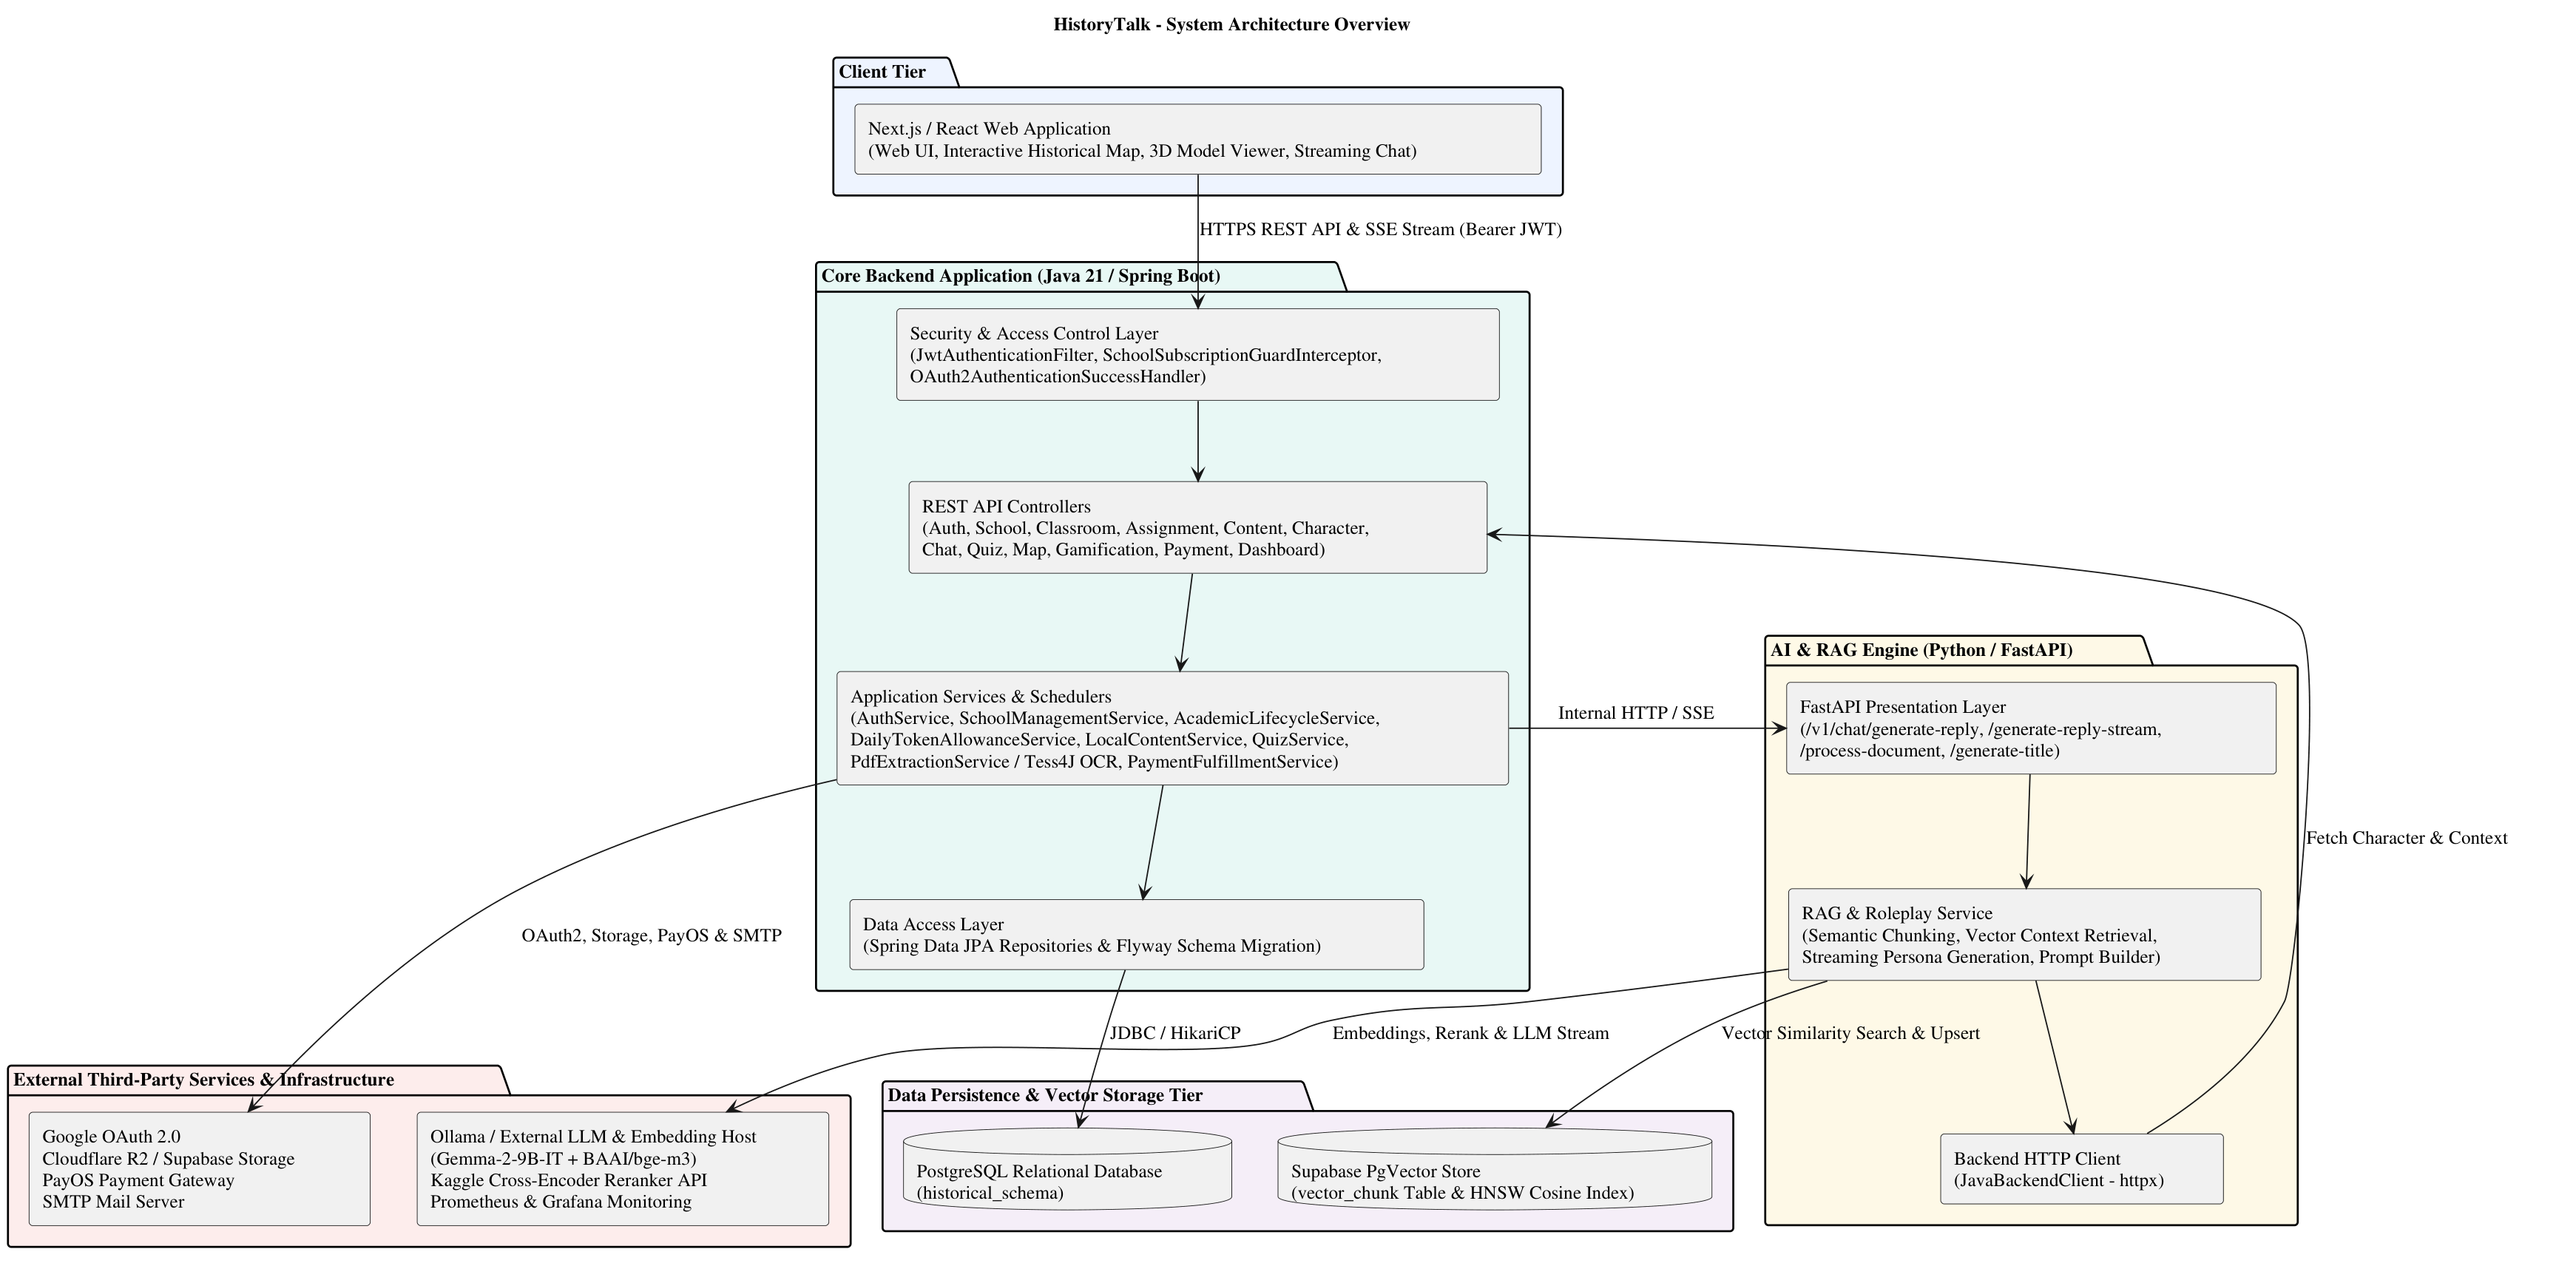
\includegraphics[width=0.92\textwidth,height=0.62\textheight,keepaspectratio]{figures/arch_system_overview.png}
    \caption{HistoryTalk System Architecture Overview}
    \label{fig:arch_system_overview}
\end{figure}

As illustrated in Figure~\ref{fig:arch_system_overview}, the system comprises four primary architectural tiers and external service integrations:

\begin{enumerate}[leftmargin=*]
    \item \textbf{Client Tier:} Provides role-tailored web workspaces for platform actors (Customer, School Student, Teacher, School Admin, Content Admin, and System Admin). It renders interactive spatio-temporal historical battle maps, 3D historical character models, Server-Sent Events (SSE) streaming AI dialogues, timed quizzes, and classroom gradebooks.
    \item \textbf{Core Backend Service:} Acts as the central transactional backend for client traffic. It handles stateless JWT authentication (Jwt\ab Authentication\ab Filter), school academic-year subscription guards (School\ab Subscription\ab Guard\ab Interceptor), multi-tenant data isolation by school\_id, PDF text and OCR extraction (Apache PDFBox and Tess4J), PayOS webhook fulfillment, and Flyway database schema migrations.
    \item \textbf{AI and Hybrid RAG Service:} A dedicated asynchronous Python FastAPI service protected by an internal API key (X-Internal-\ab Api-Key). It executes dynamic semantic chunking, generates 768-dimensional dense embeddings (BAAI/\ab bge-m3), queries Supabase PgVector for context retrieval, invokes the Kaggle Cross-Encoder Reranker, and streams grounded first-person historical persona responses with Socratic reverse-questioning.
    \item \textbf{Data Persistence and Vector Storage Tier:} Combines PostgreSQL (housing relational domain tables in historical\_\ab schema) with Supabase PgVector (storing the vector\_\ab chunk table indexed with HNSW cosine distance for semantic similarity search).
    \item \textbf{External Third-Party Integrations:} Includes Google OAuth 2.0 for Single Sign-On, Cloudflare R2 / Supabase Storage for binary media and 3D models, PayOS Payment Gateway for VietQR checkout and HMAC-SHA256 webhooks, SMTP Mail Server for transactional emails, Ollama / OpenAI-Compatible LLM Host, Kaggle Reranker API, and Prometheus with Grafana for system monitoring.
\end{enumerate}

\newpage
\subsection{Package Diagram}

\subsubsection{Back-end Core Packages}

The Java Core Backend follows a layered and domain-partitioned package organization under com.historytalk, ensuring clean separation between HTTP presentation, security filters, domain business logic, and JPA persistence.

\begin{figure}[htbp]
    \centering
    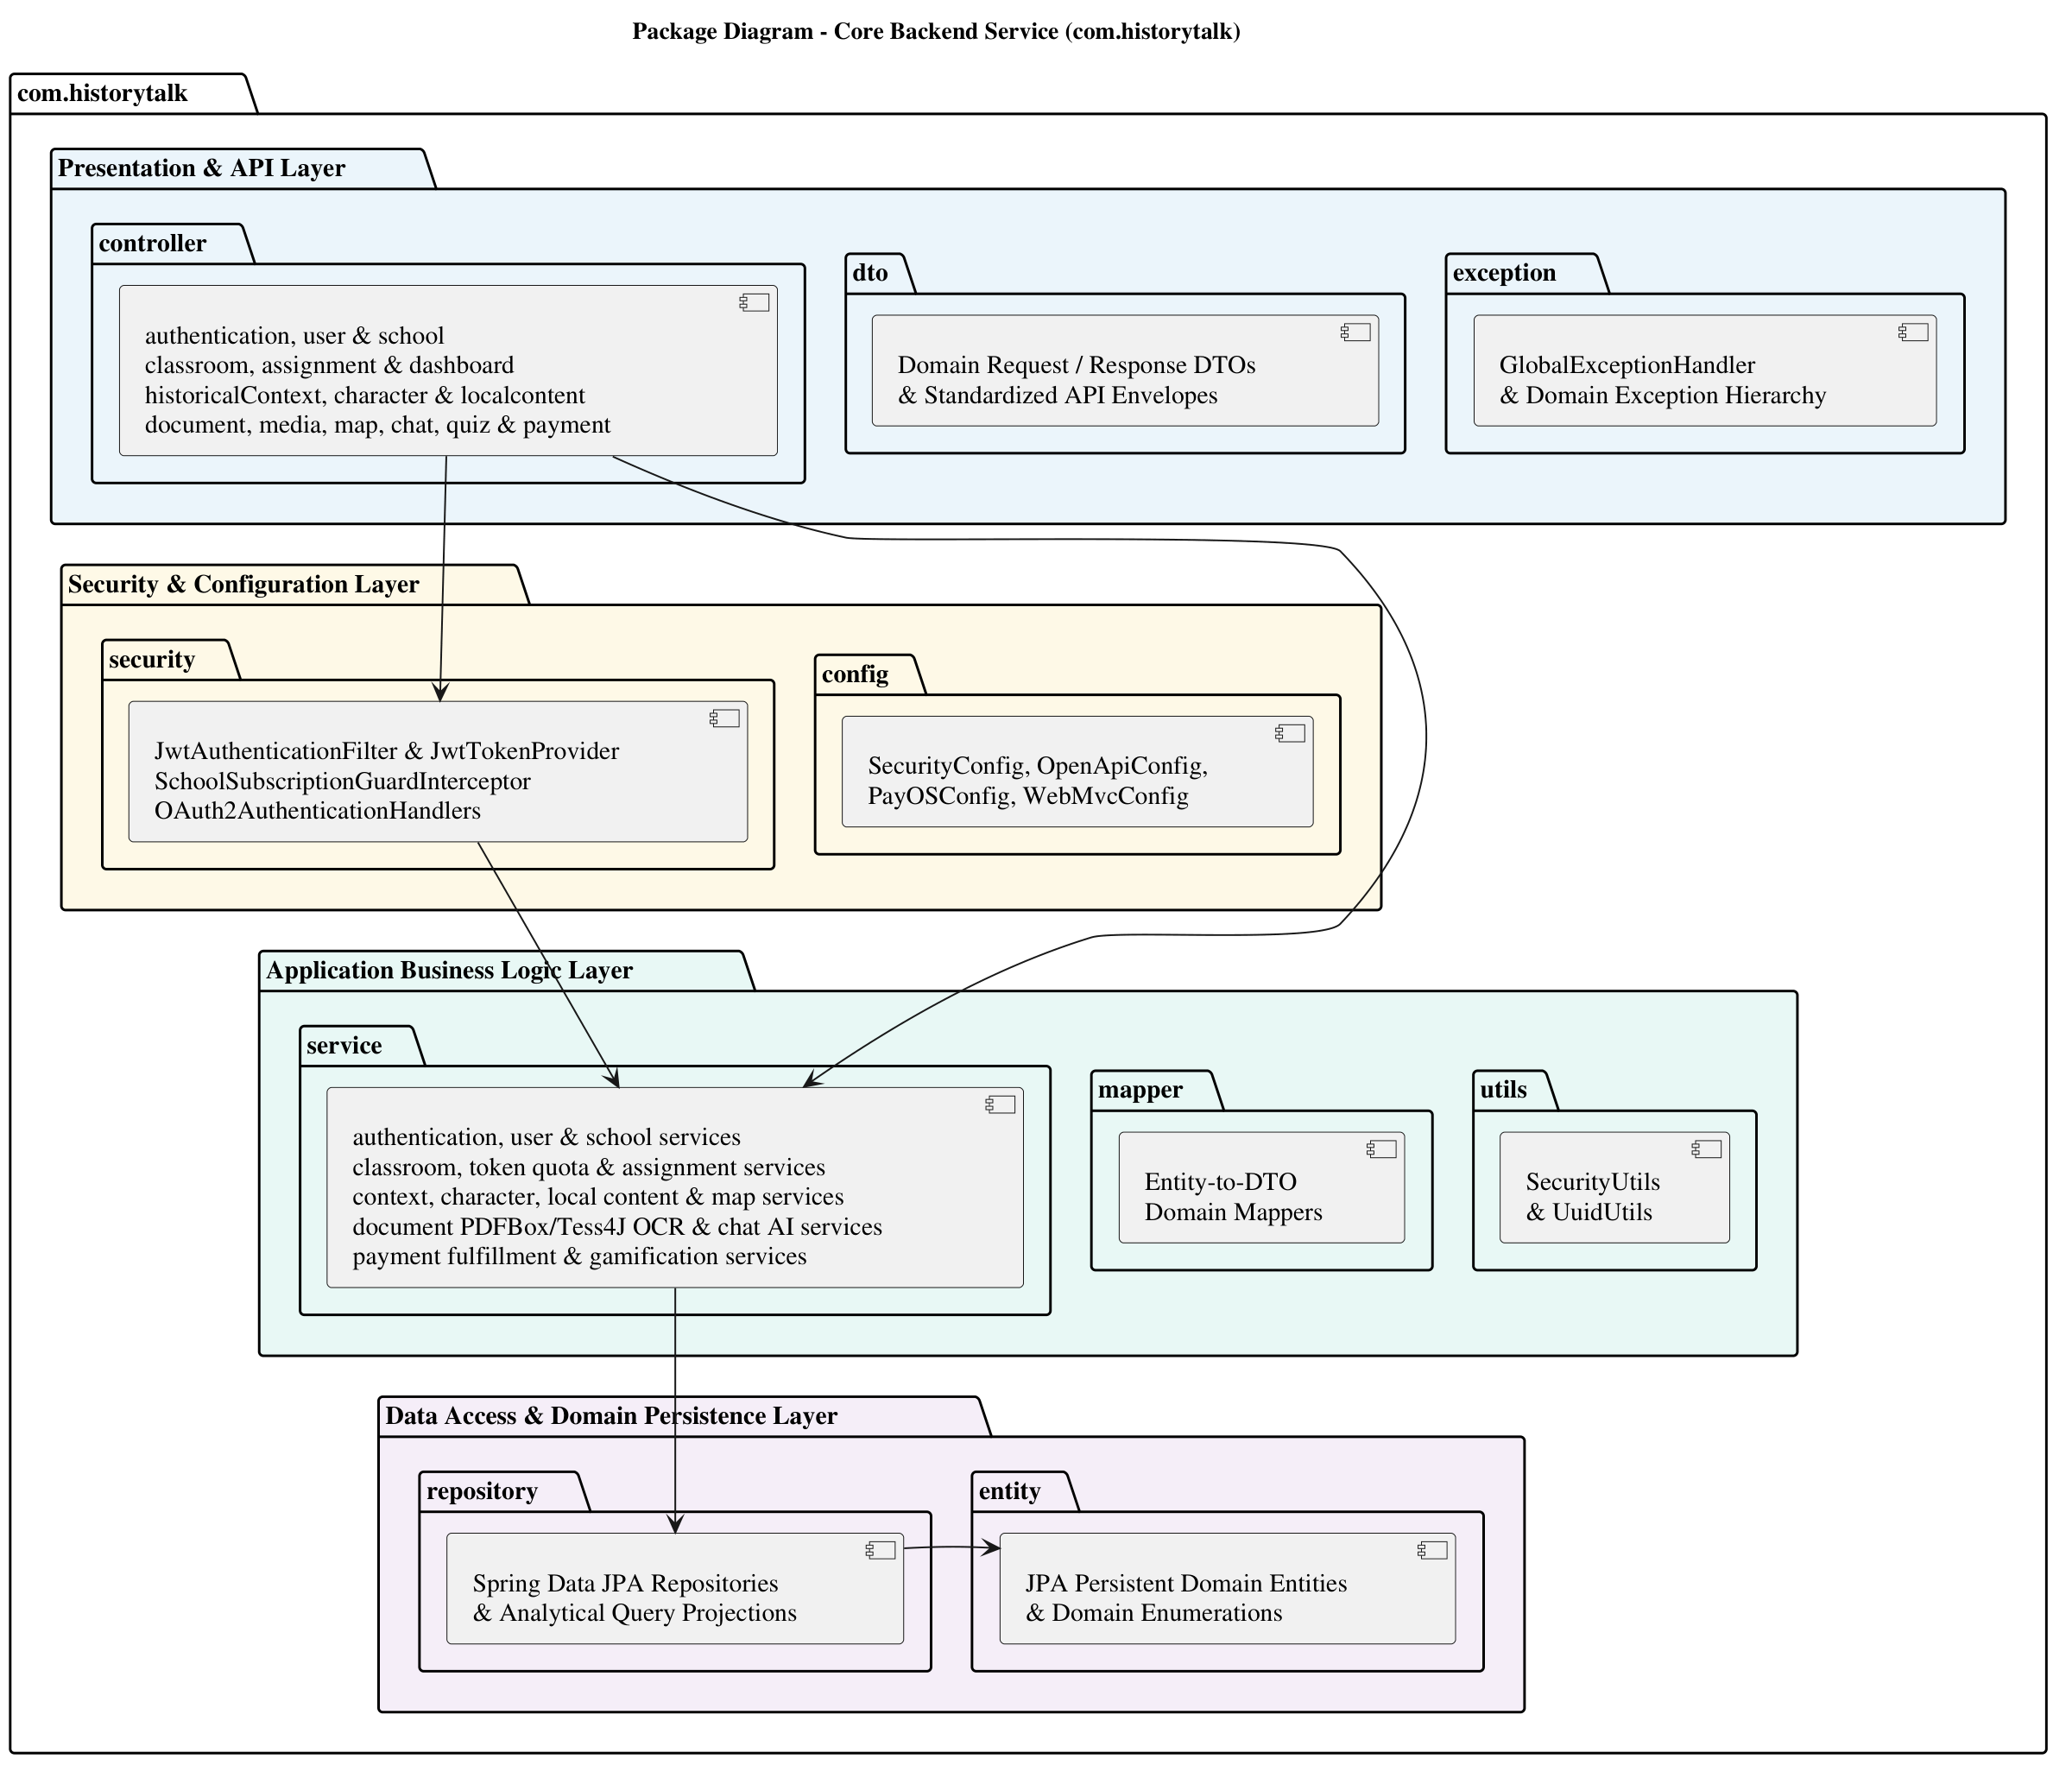
\includegraphics[width=0.88\textwidth,height=0.55\textheight,keepaspectratio]{figures/pkg_backend_java.png}
    \caption{Package Diagram -- Core Backend Service}
    \label{fig:pkg_backend_java}
\end{figure}

\paragraph{Package Descriptions}
\begin{longtable}{|C{0.9cm}|L{4.5cm}|L{8.9cm}|}
\hline
\rowcolor{tableheader}
\textbf{No} & \textbf{Package} & \textbf{Description} \\
\hline
\endhead
01 & com.historytalk.\ab config & Configures Spring Security filter chains (Security\ab Config), OpenAPI/Swagger documentation (OpenApi\ab Config), PayOS SDK client (PayOS\ab Config), OAuth2 properties (OAuth2\ab Properties), and MVC interceptors (School\ab Lifecycle\ab WebMvc\ab Config). \\
\hline
02 & com.historytalk.\ab security & Implements JWT token parsing and signing (JwtToken\ab Provider), request authentication (Jwt\ab Authentication\ab Filter), B2B school subscription enforcement (School\ab Subscription\ab Guard\ab Interceptor), and Google OAuth2 handlers (security.\ab oauth2). \\
\hline
03 & com.historytalk.\ab controller.* & Exposes RESTful API controllers grouped into domain subpackages (authentication, user, school, classroom, assignment, historical\ab Context, character, local\ab content, document, map, chat, quiz, gamification, payment, dashboard, trash). \\
\hline
04 & com.historytalk.\ab dto.* & Encapsulates strongly-typed Request and Response Data Transfer Objects across domain subpackages, along with standardized envelope wrappers (ApiResponse, Paginated\ab ApiResponse, Validation\ab ErrorResponse). \\
\hline
05 & com.historytalk.\ab service.* & Implements and manages core domain business rules, multi-tenant authorization checks, PDF/OCR processing (service.\ab document), CSV bulk student imports (service.\ab school.\ab student), daily token quota and boost workflows (service.\ab school.\ab token), AI service HTTP/SSE communication (service.\ab chat), and resilient PayOS fulfillment (service.\ab payment). \\
\hline
06 & com.historytalk.\ab mapper.* & Maps internal JPA domain entities to external DTO contracts (Character\ab Mapper, User\ab Mapper, Payment\ab Mapper, Tier\ab Mapper) without leaking persistence internals. \\
\hline
07 & com.historytalk.\ab repository.* & Defines Spring Data JPA repository interfaces and analytical query projection interfaces (repository.\ab dashboard) for system, school, and classroom analytics. \\
\hline
08 & com.historytalk.\ab entity.* & Contains persistent JPA domain entities across domain subpackages (user, school, classroom, assignment, historical\ab Context, character, local\ab content, document, map, chat, quiz, gamification, payment) and domain enumerations (entity.\ab enums). \\
\hline
09 & com.historytalk.\ab exception & Centralizes exception handling via Global\ab Exception\ab Handler and domain exception hierarchy (Base\ab Exception, Resource\ab NotFound\ab Exception, Invalid\ab Request\ab Exception, DataConflict\ab Exception, Forbidden\ab Exception, Unauthorized\ab Exception). \\
\hline
10 & com.historytalk.\ab utils & Provides cross-cutting security context helpers (Security\ab Utils) and UUID validation/conversion utilities (Uuid\ab Utils). \\
\hline
\caption{Core Backend Package Descriptions}
\label{tab:pkg_backend_java}
\end{longtable}

\subsubsection{AI and RAG Service Packages}

The Python AI service is organized under src/history\_\ab talk\_ai following a four-layer architecture (presentation, application, dataaccess, and common).

\begin{figure}[htbp]
    \centering
    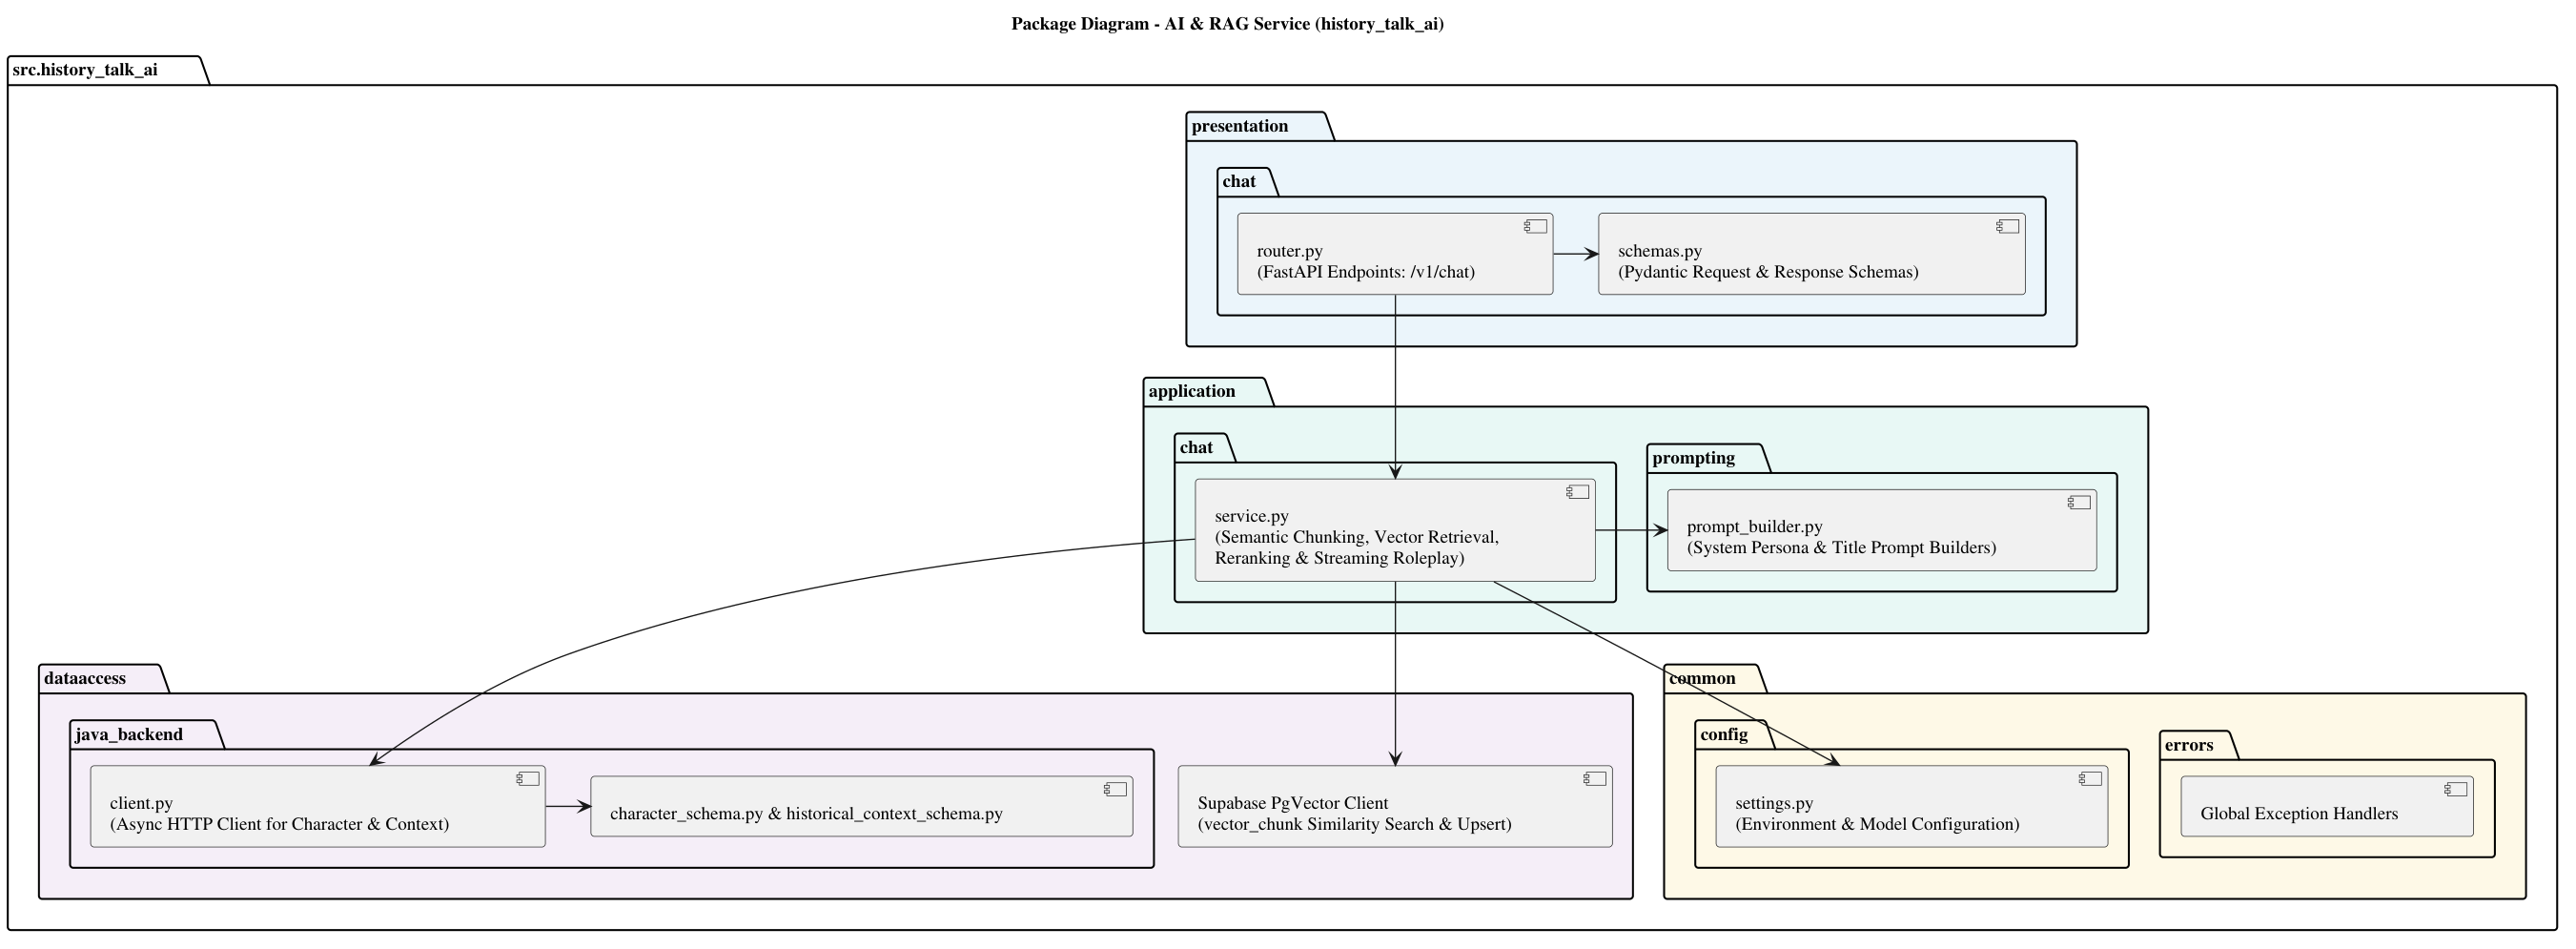
\includegraphics[width=0.85\textwidth,height=0.50\textheight,keepaspectratio]{figures/pkg_backend_ai.png}
    \caption{Package Diagram -- AI and RAG Service}
    \label{fig:pkg_backend_ai}
\end{figure}

\paragraph{Package Descriptions}
\begin{longtable}{|C{0.9cm}|L{4.5cm}|L{8.9cm}|}
\hline
\rowcolor{tableheader}
\textbf{No} & \textbf{Package} & \textbf{Description} \\
\hline
\endhead
01 & presentation.\ab chat.router & Exposes FastAPI endpoints under /v1/chat (/generate-\ab reply, /generate-\ab reply-stream, /generate-\ab title, /process-\ab document, and DELETE /documents/\ab \{doc\_id\}) secured by internal API key validation. \\
\hline
02 & presentation.\ab chat.schemas & Defines Pydantic request and response models (Generate\ab ReplyRequest, Generate\ab ReplyResponse, Message\ab HistoryItem, Process\ab Document\ab Request, Generate\ab TitleRequest). \\
\hline
03 & application.\ab chat.service & Implements the core RAG and LLM pipeline: dynamic semantic chunking (\_semantic\_\ab chunking), BGE-M3 embedding generation (get\_\ab embedding\_\ab from\_ollama), Supabase vector similarity retrieval and Kaggle reranking (retrieve\_\ab history\_\ab context), and SSE streaming roleplay (generate\_\ab reply\_\ab stream). \\
\hline
04 & application.\ab prompting & Houses prompt\_\ab builder.py (build\_chat\_\ab system\_prompt, build\_title\_\ab system\_prompt), constructing first-person historical persona instructions, anti-hallucination constraints, and Socratic questioning rules. \\
\hline
05 & dataaccess.\ab java\_backend & Implements asynchronous httpx client (client.py) and typed domain schemas (character\_\ab schema.py, historical\_\ab context\_\ab schema.py) to fetch character biographies, eras, and context metadata from the Java Core Backend. \\
\hline
06 & common.config & Manages environment configuration via pydantic-\ab settings (settings.py), binding LLM provider routing (ollama vs. external), model parameters, Supabase credentials, and timeouts. \\
\hline
07 & common.errors & Provides global FastAPI exception handlers and structured JSON error responses for upstream timeout, embedding, or LLM inference failures. \\
\hline
\caption{AI and RAG Service Package Descriptions}
\label{tab:pkg_backend_ai}
\end{longtable}

\subsubsection{Front-end Web Application Packages}

\begin{figure}[htbp]
    \centering
    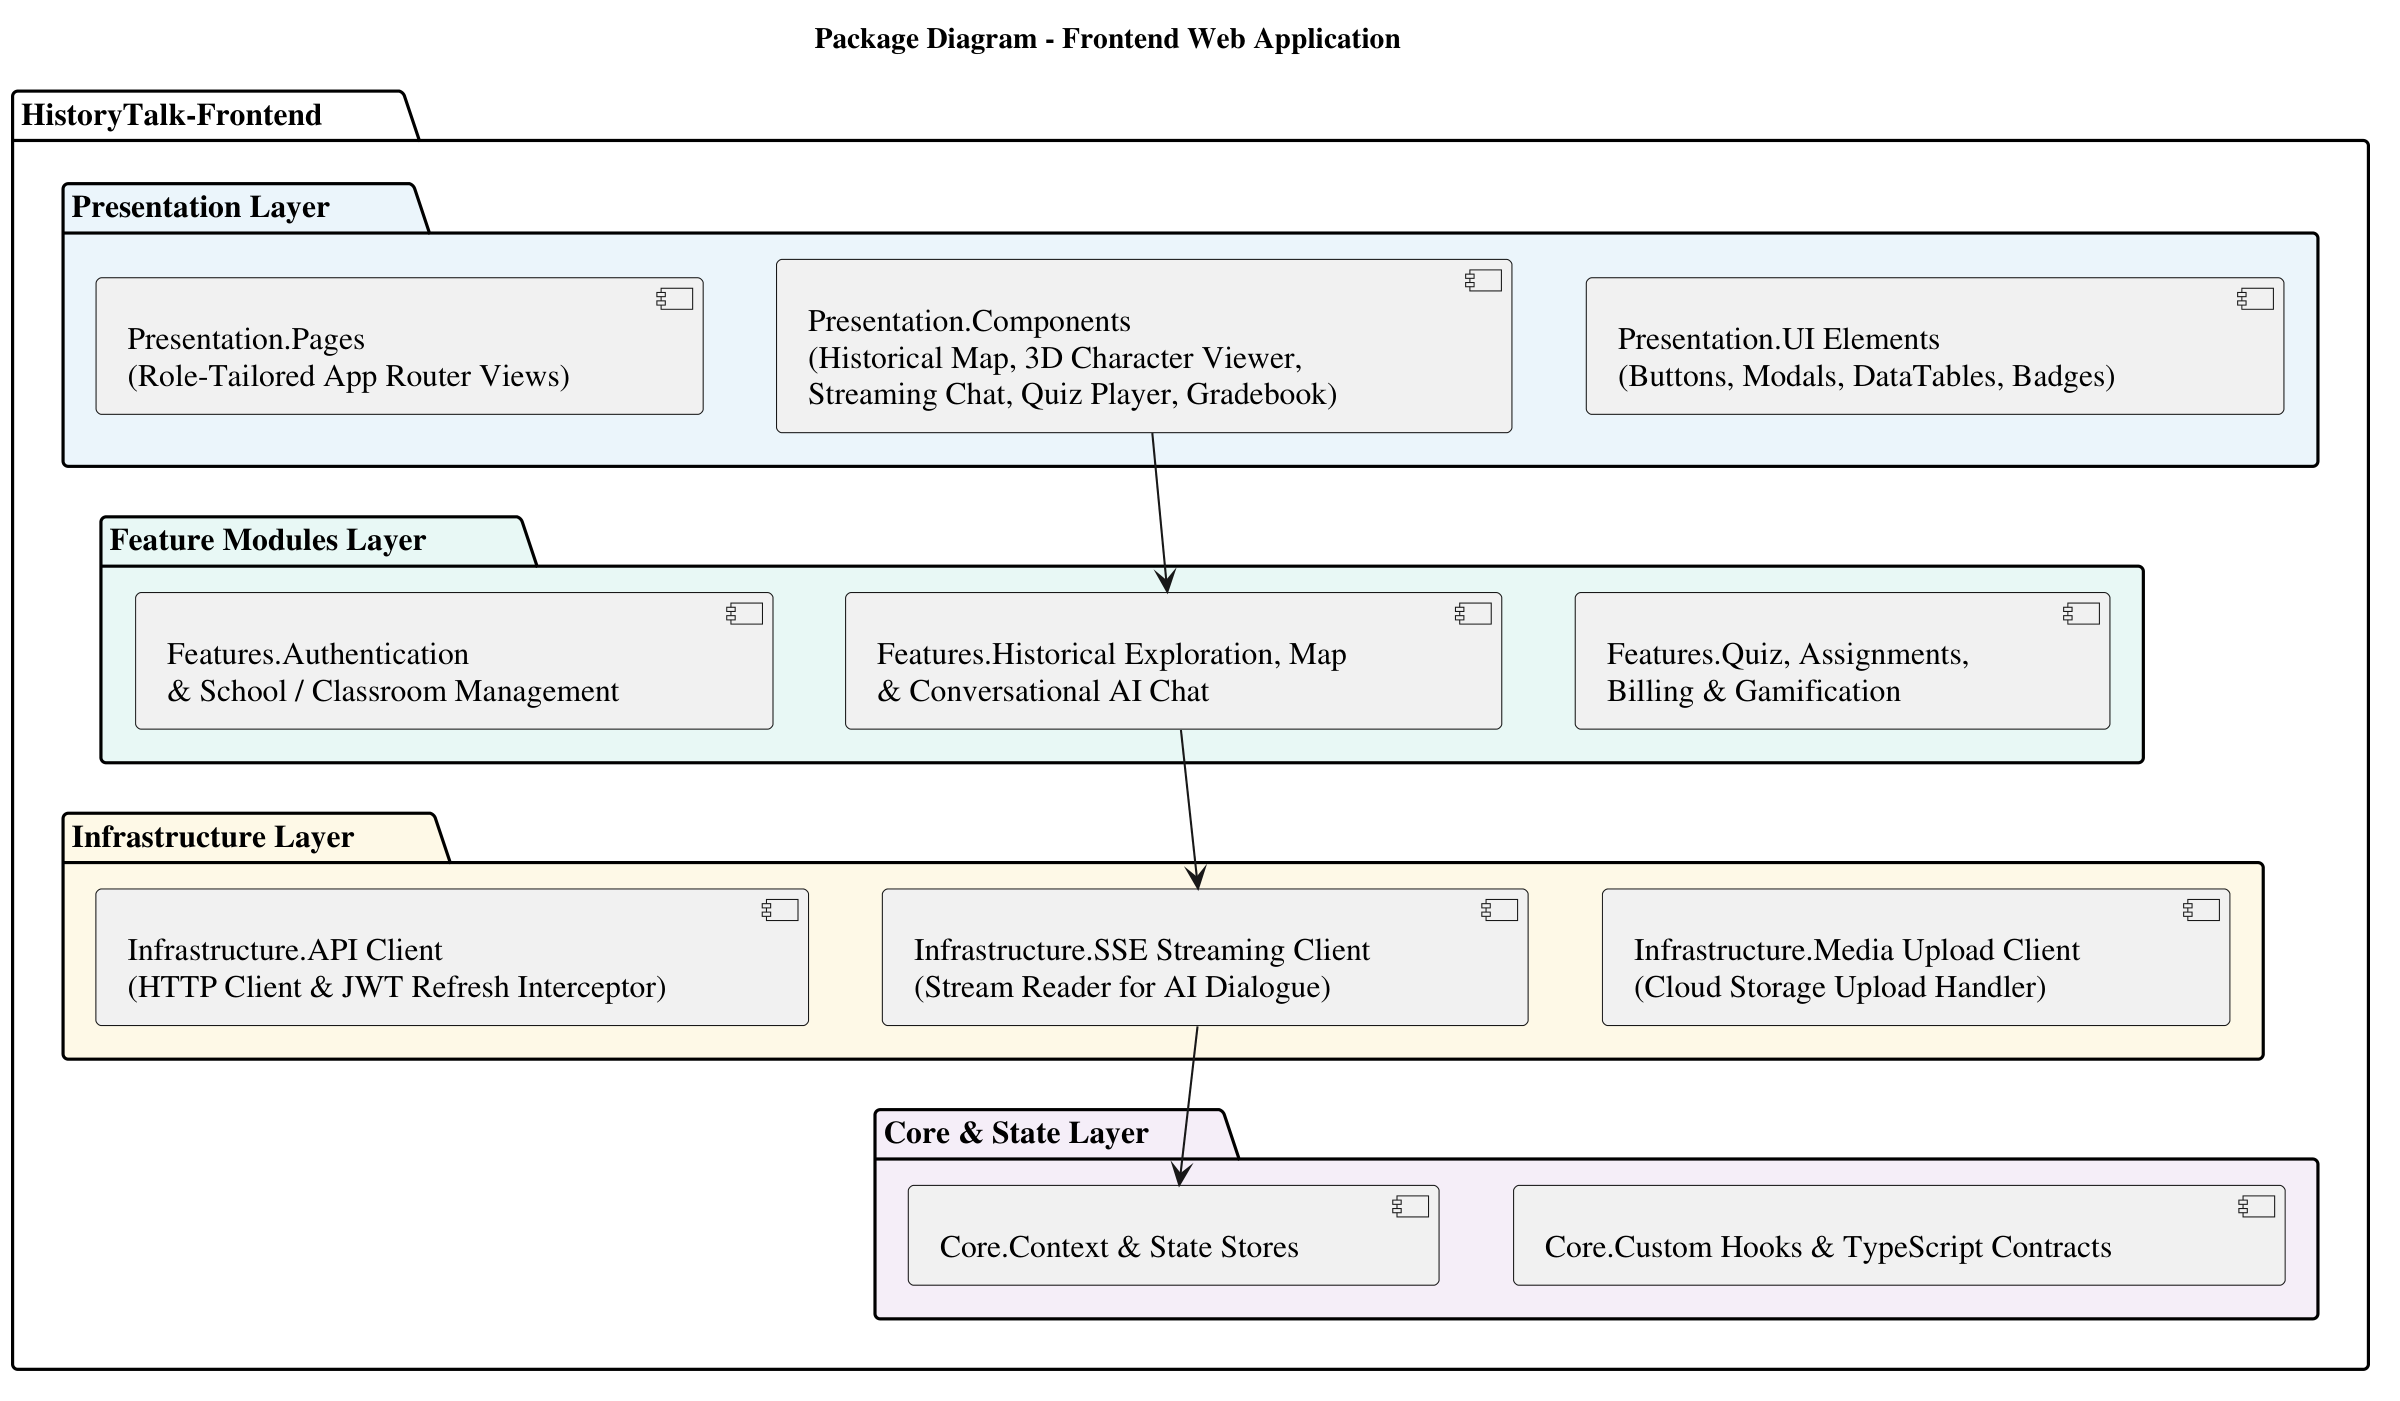
\includegraphics[width=0.88\textwidth,height=0.52\textheight,keepaspectratio]{figures/pkg_frontend_web.png}
    \caption{Package Diagram -- Frontend Web Application}
    \label{fig:pkg_frontend_web}
\end{figure}

\paragraph{Package Descriptions}
\begin{longtable}{|C{0.9cm}|L{4.5cm}|L{8.9cm}|}
\hline
\rowcolor{tableheader}
\textbf{No} & \textbf{Package} & \textbf{Description} \\
\hline
\endhead
01 & Presentation.\ab Pages & Next.js App Router views segregated by actor role: Public/Customer Portal, School Student Learning Workspace, Teacher Classroom Console, School Admin Portal, Content Admin Studio, and System Admin Dashboard. \\
\hline
02 & Presentation.\ab Components & Reusable domain widgets including BattleMap\ab Canvas (interactive map pins and animated route arrows), Character3D\ab Viewer (3D model viewer), Streaming\ab ChatBox, QuizPlayer, and Gradebook\ab Table. \\
\hline
03 & Presentation.\ab UI Elements & Atomic design primitives (Buttons, Dialog Modals, DataTables, Pagination, StatusBadges, Toast notifications, and Skeletons). \\
\hline
04 & Features.\ab Authentication & Handles credential login, Google OAuth2 callback processing, mandatory first-login password change for imported school students, and role-based route protection. \\
\hline
05 & Features.\ab School \& Classroom & Manages B2B school onboarding, academic year lifecycle rollover, classroom creation, CSV student roster bulk import, and daily token quota/boost review workflows. \\
\hline
06 & Features.\ab Historical Exploration \& Map & Drives timeline browsing by EventEra and Event\ab Category, interactive battle-map overlays, camera viewpoint focuses (MapFocus), and school-owned local history content workflows. \\
\hline
07 & Features.\ab Conversational AI Chat & Manages character roleplay sessions, real-time SSE token streaming, clickable suggested follow-up questions, and cited historical quotes display. \\
\hline
08 & Features.\ab Quiz \& Assignments & Implements interactive quiz players (MULTIPLE\_\ab CHOICE, FILL\_IN\_\ab BLANK, MATCHING), question bank CSV import, teacher assignment dispatch, and automated submission tracking. \\
\hline
09 & Features.\ab Billing \& Gamification & Manages B2C tier upgrades via PayOS QR checkout, order status polling, daily streak check-ins, and daily quest token rewards. \\
\hline
10 & Infrastructure & Configures HTTP client interceptors with automatic JWT refresh token rotation, SSE stream readers, and direct binary media uploads to cloud storage. \\
\hline
11 & Core / State & Provides React contexts, state stores, custom hooks (useAuth, useStreaming\ab Chat, useToken\ab Balance), and TypeScript DTO interfaces synchronized with backend API specs. \\
\hline
\caption{Frontend Web Application Package Descriptions}
\label{tab:pkg_frontend_web}
\end{longtable}

\newpage
% ============================================================================
% SECTION 2: DATABASE DESIGN
% ============================================================================
\section{Database Design}

\subsection{Entity-Relationship Diagram (Logical \& Physical ERD)}

The HistoryTalk persistence layer is built on \textbf{PostgreSQL 16} (relational schema \texttt{historical\_\ab schema}) integrated with \textbf{Supabase PgVector} (vector extension \texttt{vector(768)} with HNSW indexing). Schema evolution is strictly version-controlled through \textbf{Flyway Migrations (\texttt{V1} to \texttt{V38})}. Across all 6 bounded domains, the database comprises \textbf{32 tables} (30 JPA entity tables, 1 many-to-many join table \texttt{context\_\ab character\_\ab mapping}, and 1 vector store table \texttt{vector\_\ab chunk}).

\begin{figure}[htbp]
    \centering
    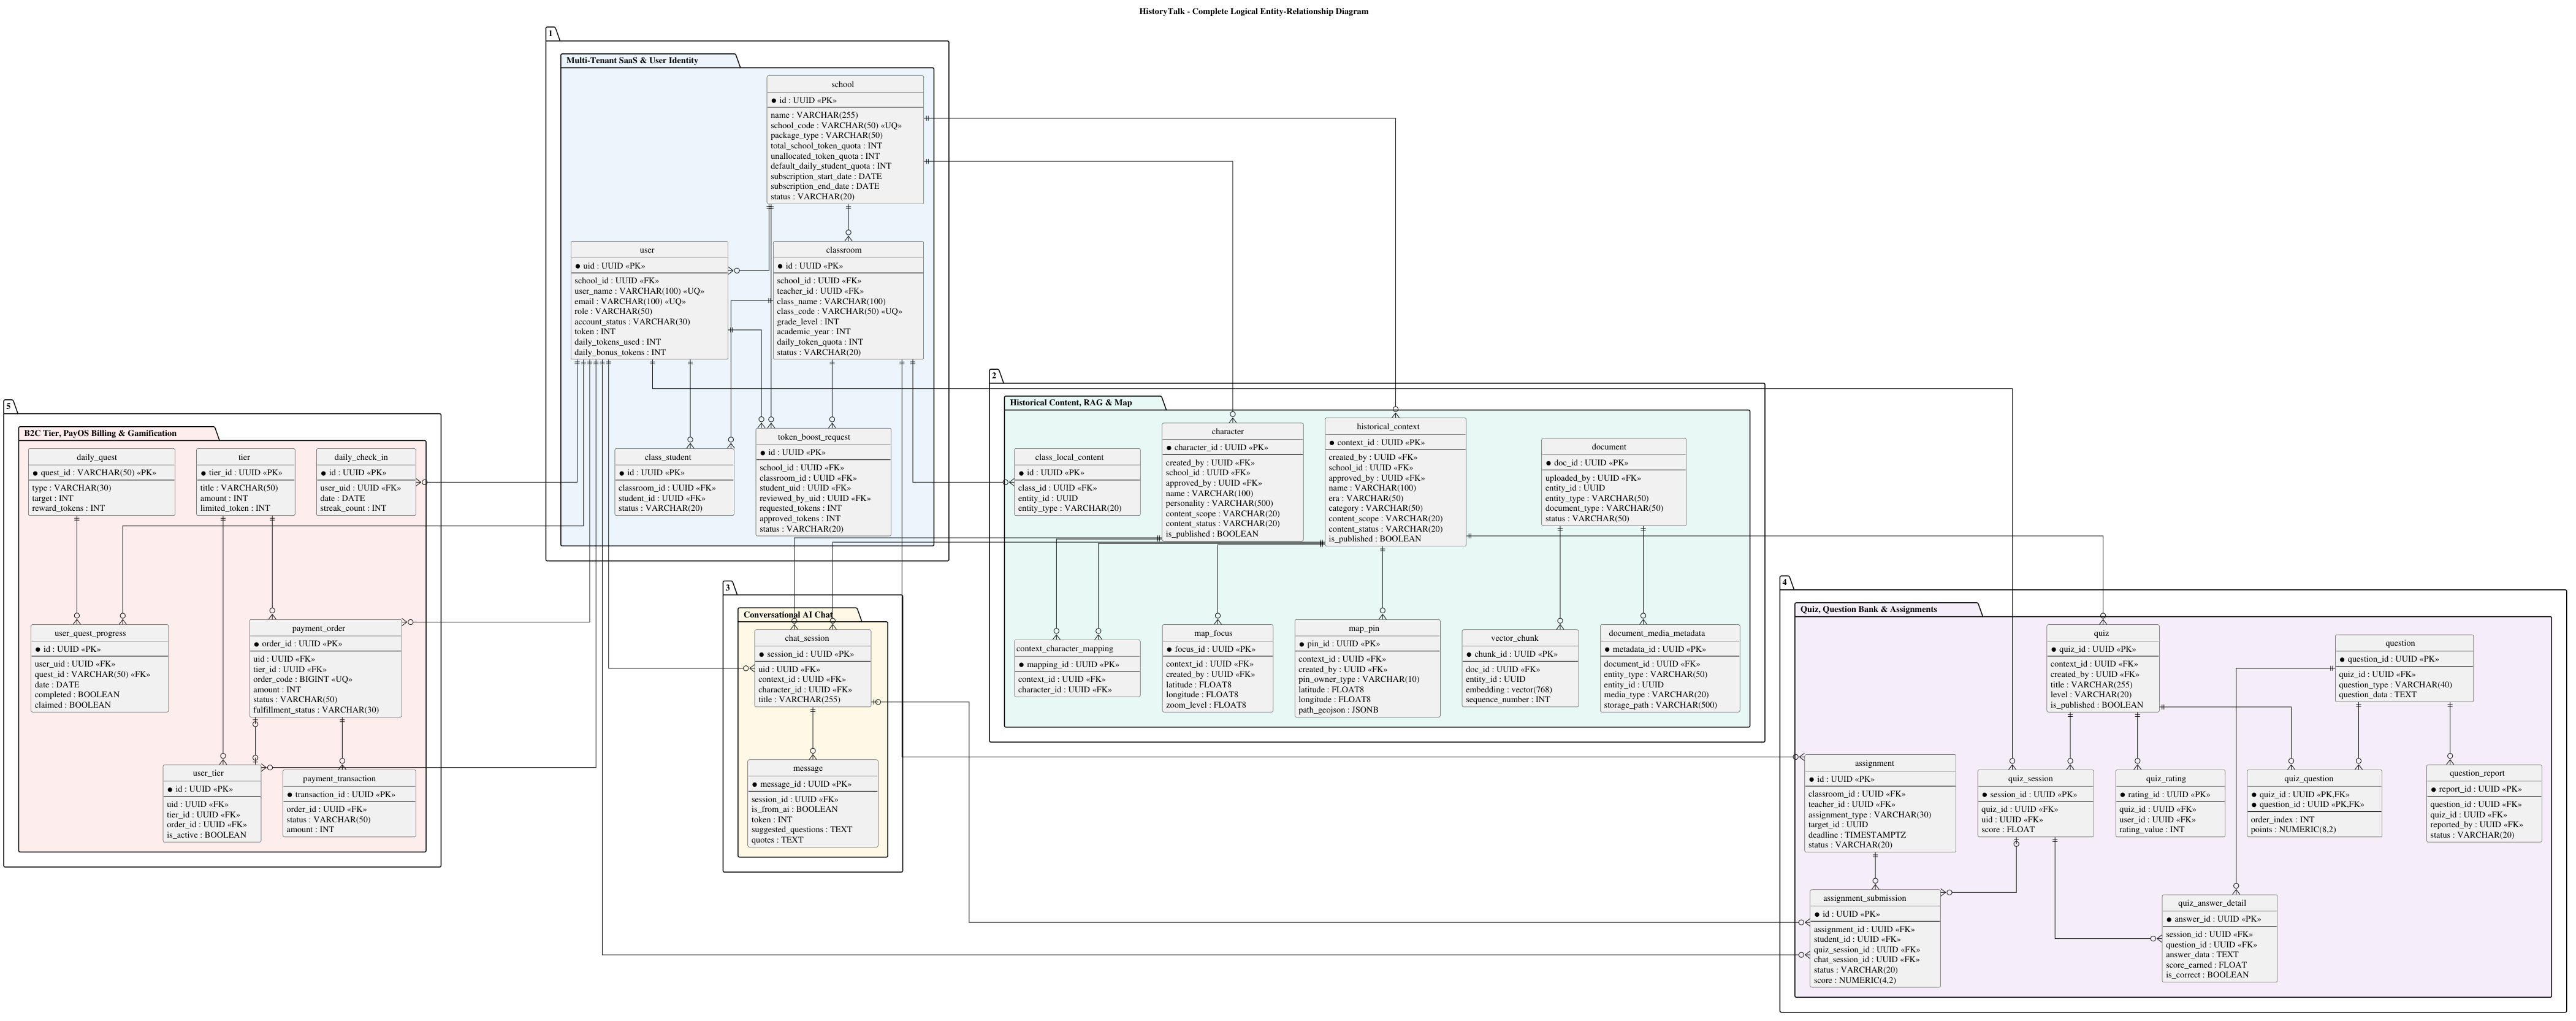
\includegraphics[width=0.99\textwidth,height=0.70\textheight,keepaspectratio]{figures/erd_full_overview.png}
    \caption{Complete Logical Entity-Relationship Diagram (32 Database Tables across 6 Bounded Domains)}
    \label{fig:erd_full_overview}
\end{figure}

\newpage
\subsection{Table Descriptions}

Table~\ref{tab:db_table_descriptions} summarizes all 32 database tables in HistoryTalk, specifying the business purpose, Primary Keys (PK), and Foreign Keys (FK) of each table in alignment with the database migration scripts and JPA entity models.

\begin{longtable}{|C{0.9cm}|L{4.2cm}|L{9.2cm}|}
\hline
\rowcolor{tableheader}
\textbf{No} & \textbf{Table} & \textbf{Description} \\
\hline
\endhead
01 & \texttt{school} & Stores B2B multi-tenant school organizations, enterprise subscription packages (\texttt{ENTERPRISE\_\ab SMALL}, \texttt{ENTERPRISE\_\ab MEDIUM}, \texttt{ENTERPRISE\_\ab LARGE}), shared token pools, academic subscription dates (\texttt{01/09}--\texttt{31/05}), and default daily student token quotas.\newline
$\bullet$ \textbf{Primary keys:} \texttt{id}\newline
$\bullet$ \textbf{Foreign keys:} None \\
\hline
02 & \texttt{"user"} & Stores all platform user accounts across 6 RBAC roles (\texttt{CUSTOMER}, \texttt{CONTENT\_\ab ADMIN}, \texttt{SYSTEM\_\ab ADMIN}, \texttt{SCHOOL\_\ab ADMIN}, \texttt{TEACHER}, \texttt{SCHOOL\_\ab STUDENT}), credentials, account status, B2C token balance, and B2B daily token consumption.\newline
$\bullet$ \textbf{Primary keys:} \texttt{uid}\newline
$\bullet$ \textbf{Foreign keys:} \texttt{school\_\ab id} $\rightarrow$ \texttt{school(id)} \\
\hline
03 & \texttt{classroom} & Represents school classrooms managed by teachers for a specific grade level (6--12) and academic year, with optional per-classroom daily token quota overrides.\newline
$\bullet$ \textbf{Primary keys:} \texttt{id}\newline
$\bullet$ \textbf{Foreign keys:} \texttt{school\_\ab id} $\rightarrow$ \texttt{school(id)}, \texttt{teacher\_\ab id} $\rightarrow$ \texttt{"user"(uid)} \\
\hline
04 & \texttt{class\_\ab student} & Junction table mapping enrolled school students to classrooms with enrollment timestamps and active status.\newline
$\bullet$ \textbf{Primary keys:} \texttt{id}\newline
$\bullet$ \textbf{Foreign keys:} \texttt{classroom\_\ab id} $\rightarrow$ \texttt{classroom(id)}, \texttt{student\_\ab id} $\rightarrow$ \texttt{"user"(uid)} \\
\hline
05 & \texttt{token\_\ab boost\_\ab request} & Tracks daily token boost requests submitted by school students when reaching their daily quota, and approval/rejection records by teachers or school admins.\newline
$\bullet$ \textbf{Primary keys:} \texttt{id}\newline
$\bullet$ \textbf{Foreign keys:} \texttt{school\_\ab id} $\rightarrow$ \texttt{school(id)}, \texttt{classroom\_\ab id} $\rightarrow$ \texttt{classroom(id)}, \texttt{student\_\ab uid} $\rightarrow$ \texttt{"user"(uid)}, \texttt{reviewed\_\ab by\_\ab uid} $\rightarrow$ \texttt{"user"(uid)} \\
\hline
06 & \texttt{historical\_\ab context} & Stores historical events, eras (\texttt{ANCIENT}, \texttt{MEDIEVAL}, \texttt{MODERN}, \texttt{CONTEMPORARY}), categories, GeoJSON battle-map overlays, and multi-tenant local content approval states.\newline
$\bullet$ \textbf{Primary keys:} \texttt{context\_\ab id}\newline
$\bullet$ \textbf{Foreign keys:} \texttt{created\_\ab by} $\rightarrow$ \texttt{"user"(uid)}, \texttt{school\_\ab id} $\rightarrow$ \texttt{school(id)}, \texttt{approved\_\ab by} $\rightarrow$ \texttt{"user"(uid)} \\
\hline
07 & \texttt{"character"} & Stores historical figure personas, biographical backgrounds, speaking styles/personalities, 2D avatars, 3D model URLs (\texttt{.glb}), lifespan dates, and local content approval states.\newline
$\bullet$ \textbf{Primary keys:} \texttt{character\_\ab id}\newline
$\bullet$ \textbf{Foreign keys:} \texttt{created\_\ab by} $\rightarrow$ \texttt{"user"(uid)}, \texttt{school\_\ab id} $\rightarrow$ \texttt{school(id)}, \texttt{approved\_\ab by} $\rightarrow$ \texttt{"user"(uid)} \\
\hline
08 & \texttt{context\_\ab character\_\ab mapping} & Many-to-many bridge table associating historical characters with one or more historical contexts/campaigns.\newline
$\bullet$ \textbf{Primary keys:} \texttt{mapping\_\ab id}\newline
$\bullet$ \textbf{Foreign keys:} \texttt{context\_\ab id} $\rightarrow$ \texttt{historical\_\ab context(context\_\ab id)}, \texttt{character\_\ab id} $\rightarrow$ \texttt{"character"(character\_\ab id)} \\
\hline
09 & \texttt{class\_\ab local\_\ab content} & Assigns school-owned local historical contexts or characters (\texttt{CLASS\_\ab ONLY} or \texttt{SCHOOL\_\ab WIDE}) to specific classrooms.\newline
$\bullet$ \textbf{Primary keys:} \texttt{id}\newline
$\bullet$ \textbf{Foreign keys:} \texttt{class\_\ab id} $\rightarrow$ \texttt{classroom(id)}, \texttt{assigned\_\ab by} $\rightarrow$ \texttt{"user"(uid)} \\
\hline
10 & \texttt{document} & Stores reference historical documents (\texttt{TEXT}, \texttt{MARKDOWN}, \texttt{PDF}, \texttt{IMAGE\_\ab 2D}, \texttt{IMAGE\_\ab 3D}) attached polymorphically to contexts or characters for RAG grounding.\newline
$\bullet$ \textbf{Primary keys:} \texttt{doc\_\ab id}\newline
$\bullet$ \textbf{Foreign keys:} \texttt{uploaded\_\ab by} $\rightarrow$ \texttt{"user"(uid)} \\
\hline
11 & \texttt{document\_\ab media\_\ab metadata} & Polymorphic media metadata table storing Cloudflare R2 / Supabase Storage paths, dimensions, file sizes, and formats for characters, contexts, documents, and avatars.\newline
$\bullet$ \textbf{Primary keys:} \texttt{metadata\_\ab id}\newline
$\bullet$ \textbf{Foreign keys:} \texttt{document\_\ab id} $\rightarrow$ \texttt{document(doc\_\ab id)} \\
\hline
12 & \texttt{vector\_\ab chunk} & Supabase PgVector table storing semantically chunked document passages and 768-dimensional \texttt{BAAI/bge-m3} embeddings indexed with HNSW cosine similarity.\newline
$\bullet$ \textbf{Primary keys:} \texttt{chunk\_\ab id}\newline
$\bullet$ \textbf{Foreign keys:} \texttt{doc\_\ab id} $\rightarrow$ \texttt{document(doc\_\ab id)} \\
\hline
13 & \texttt{map\_\ab pin} & Stores interactive map markers (\texttt{ADMIN} or \texttt{USER} owned), coordinates, historical years, and GeoJSON \texttt{LineString} troop movement paths for a historical context.\newline
$\bullet$ \textbf{Primary keys:} \texttt{pin\_\ab id}\newline
$\bullet$ \textbf{Foreign keys:} \texttt{context\_\ab id} $\rightarrow$ \texttt{historical\_\ab context(context\_\ab id)}, \texttt{created\_\ab by} $\rightarrow$ \texttt{"user"(uid)} \\
\hline
14 & \texttt{map\_\ab focus} & Stores predefined camera viewpoints (latitude, longitude, zoom level, display order) to guide learners through key geographical stages of a campaign.\newline
$\bullet$ \textbf{Primary keys:} \texttt{focus\_\ab id}\newline
$\bullet$ \textbf{Foreign keys:} \texttt{context\_\ab id} $\rightarrow$ \texttt{historical\_\ab context(context\_\ab id)}, \texttt{created\_\ab by} $\rightarrow$ \texttt{"user"(uid)} \\
\hline
15 & \texttt{chat\_\ab session} & Tracks conversational AI roleplay sessions between a user and a historical character within a specific historical context.\newline
$\bullet$ \textbf{Primary keys:} \texttt{session\_\ab id}\newline
$\bullet$ \textbf{Foreign keys:} \texttt{uid} $\rightarrow$ \texttt{"user"(uid)}, \texttt{context\_\ab id} $\rightarrow$ \texttt{historical\_\ab context(context\_\ab id)}, \texttt{character\_\ab id} $\rightarrow$ \texttt{"character"(character\_\ab id)} \\
\hline
16 & \texttt{message} & Stores individual user and AI dialogue turns within a chat session, including token usage, 3 AI-suggested follow-up questions, and cited RAG historical quotes.\newline
$\bullet$ \textbf{Primary keys:} \texttt{message\_\ab id}\newline
$\bullet$ \textbf{Foreign keys:} \texttt{session\_\ab id} $\rightarrow$ \texttt{chat\_\ab session(session\_\ab id)} \\
\hline
17 & \texttt{quiz} & Stores assessment quizzes linked to historical contexts, categorized by difficulty level (\texttt{EASY}, \texttt{MEDIUM}, \texttt{HARD}) and publication status.\newline
$\bullet$ \textbf{Primary keys:} \texttt{quiz\_\ab id}\newline
$\bullet$ \textbf{Foreign keys:} \texttt{context\_\ab id} $\rightarrow$ \texttt{historical\_\ab context(context\_\ab id)}, \texttt{created\_\ab by} $\rightarrow$ \texttt{"user"(uid)} \\
\hline
18 & \texttt{question} & Central question bank supporting three polymorphic question types (\texttt{MULTIPLE\_\ab CHOICE}, \texttt{FILL\_\ab IN\_\ab BLANK}, \texttt{MATCHING}) with JSON payload \texttt{question\_\ab data} and explanations.\newline
$\bullet$ \textbf{Primary keys:} \texttt{question\_\ab id}\newline
$\bullet$ \textbf{Foreign keys:} \texttt{quiz\_\ab id} $\rightarrow$ \texttt{quiz(quiz\_\ab id)} (nullable for bank questions) \\
\hline
19 & \texttt{quiz\_\ab question} & Many-to-many link table binding reusable Question Bank items to Quizzes with explicit \texttt{order\_\ab index} and point weights (\texttt{points}).\newline
$\bullet$ \textbf{Primary keys:} \texttt{(quiz\_\ab id, question\_\ab id)}\newline
$\bullet$ \textbf{Foreign keys:} \texttt{quiz\_\ab id} $\rightarrow$ \texttt{quiz(quiz\_\ab id)}, \texttt{question\_\ab id} $\rightarrow$ \texttt{question(question\_\ab id)} \\
\hline
20 & \texttt{quiz\_\ab session} & Records a learner's timed quiz attempt, start/end timestamps, time limit, and final calculated score on a 10-point scale.\newline
$\bullet$ \textbf{Primary keys:} \texttt{session\_\ab id}\newline
$\bullet$ \textbf{Foreign keys:} \texttt{quiz\_\ab id} $\rightarrow$ \texttt{quiz(quiz\_\ab id)}, \texttt{uid} $\rightarrow$ \texttt{"user"(uid)} \\
\hline
21 & \texttt{quiz\_\ab answer\_\ab detail} & Stores per-question submitted answer JSON (\texttt{answer\_\ab data}), correctness flag, and points earned within a quiz attempt session.\newline
$\bullet$ \textbf{Primary keys:} \texttt{answer\_\ab id}\newline
$\bullet$ \textbf{Foreign keys:} \texttt{session\_\ab id} $\rightarrow$ \texttt{quiz\_\ab session(session\_\ab id)}, \texttt{question\_\ab id} $\rightarrow$ \texttt{question(question\_\ab id)} \\
\hline
22 & \texttt{quiz\_\ab rating} & Stores 1--5 star ratings submitted by learners after completing a quiz (enforcing one rating per user per quiz).\newline
$\bullet$ \textbf{Primary keys:} \texttt{rating\_\ab id}\newline
$\bullet$ \textbf{Foreign keys:} \texttt{quiz\_\ab id} $\rightarrow$ \texttt{quiz(quiz\_\ab id)}, \texttt{user\_\ab id} $\rightarrow$ \texttt{"user"(uid)} \\
\hline
23 & \texttt{question\_\ab report} & Stores learner/teacher error reports flagging factual or formatting issues on specific quiz questions for Content Admin review.\newline
$\bullet$ \textbf{Primary keys:} \texttt{report\_\ab id}\newline
$\bullet$ \textbf{Foreign keys:} \texttt{question\_\ab id} $\rightarrow$ \texttt{question(question\_\ab id)}, \texttt{quiz\_\ab id} $\rightarrow$ \texttt{quiz(quiz\_\ab id)}, \texttt{reported\_\ab by} $\rightarrow$ \texttt{"user"(uid)} \\
\hline
24 & \texttt{assignment} & Stores classroom homework assignments created by teachers across three learning modes (\texttt{CONTEXT\_\ab READING}, \texttt{AI\_\ab CHAT\_\ab ROLEPLAY}, \texttt{QUIZ\_\ab TEST}) with deadlines and minimum completion thresholds.\newline
$\bullet$ \textbf{Primary keys:} \texttt{id}\newline
$\bullet$ \textbf{Foreign keys:} \texttt{classroom\_\ab id} $\rightarrow$ \texttt{classroom(id)}, \texttt{teacher\_\ab id} $\rightarrow$ \texttt{"user"(uid)} \\
\hline
25 & \texttt{assignment\_\ab submission} & Tracks individual student progress, submission status (\texttt{NOT\_\ab STARTED}, \texttt{IN\_\ab PROGRESS}, \texttt{SUBMITTED}, \texttt{LATE\_\ab SUBMITTED}, \texttt{MISSED}, \texttt{EXEMPTED}), score, AI chat message count, and reading duration.\newline
$\bullet$ \textbf{Primary keys:} \texttt{id}\newline
$\bullet$ \textbf{Foreign keys:} \texttt{assignment\_\ab id} $\rightarrow$ \texttt{assignment(id)}, \texttt{student\_\ab id} $\rightarrow$ \texttt{"user"(uid)}, \texttt{quiz\_\ab session\_\ab id} $\rightarrow$ \texttt{quiz\_\ab session(session\_\ab id)}, \texttt{chat\_\ab session\_\ab id} $\rightarrow$ \texttt{chat\_\ab session(session\_\ab id)} \\
\hline
26 & \texttt{tier} & Defines B2C subscription plans (e.g., Free, Plus, Pro), pricing in VND, billing duration in months, and token allowances.\newline
$\bullet$ \textbf{Primary keys:} \texttt{tier\_\ab id}\newline
$\bullet$ \textbf{Foreign keys:} None \\
\hline
27 & \texttt{user\_\ab tier} & Records active and historical B2C tier subscriptions for users, linking to the originating \texttt{payment\_\ab order}.\newline
$\bullet$ \textbf{Primary keys:} \texttt{id}\newline
$\bullet$ \textbf{Foreign keys:} \texttt{uid} $\rightarrow$ \texttt{"user"(uid)}, \texttt{tier\_\ab id} $\rightarrow$ \texttt{tier(tier\_\ab id)}, \texttt{order\_\ab id} $\rightarrow$ \texttt{payment\_\ab order(order\_\ab id)} \\
\hline
28 & \texttt{payment\_\ab order} & Tracks PayOS checkout orders, unique numeric \texttt{order\_\ab code}, QR checkout URLs, payment status (\texttt{PENDING}, \texttt{PAID}, \texttt{CANCELLED}, \texttt{EXPIRED}, \texttt{FAILED}), and resilient fulfillment state (\texttt{PENDING}, \texttt{PROCESSING}, \texttt{FULFILLED}, \texttt{FAILED}).\newline
$\bullet$ \textbf{Primary keys:} \texttt{order\_\ab id}\newline
$\bullet$ \textbf{Foreign keys:} \texttt{uid} $\rightarrow$ \texttt{"user"(uid)}, \texttt{tier\_\ab id} $\rightarrow$ \texttt{tier(tier\_\ab id)} \\
\hline
29 & \texttt{payment\_\ab transaction} & Immutable audit log of incoming PayOS webhook payloads, bank reference numbers, and verification statuses.\newline
$\bullet$ \textbf{Primary keys:} \texttt{transaction\_\ab id}\newline
$\bullet$ \textbf{Foreign keys:} \texttt{order\_\ab id} $\rightarrow$ \texttt{payment\_\ab order(order\_\ab id)} \\
\hline
30 & \texttt{daily\_\ab quest} & Master catalog of daily gamification quests (\texttt{CHAT}, \texttt{QUIZ}, \texttt{READ\_\ab CONTEXT}), completion targets, and token rewards.\newline
$\bullet$ \textbf{Primary keys:} \texttt{quest\_\ab id}\newline
$\bullet$ \textbf{Foreign keys:} None \\
\hline
31 & \texttt{user\_\ab quest\_\ab progress} & Tracks daily per-user progress toward active quests and reward claim status.\newline
$\bullet$ \textbf{Primary keys:} \texttt{id}\newline
$\bullet$ \textbf{Foreign keys:} \texttt{user\_\ab uid} $\rightarrow$ \texttt{"user"(uid)}, \texttt{quest\_\ab id} $\rightarrow$ \texttt{daily\_\ab quest(quest\_\ab id)} \\
\hline
32 & \texttt{daily\_\ab check\_\ab in} & Records daily user login check-ins and consecutive day streak counts.\newline
$\bullet$ \textbf{Primary keys:} \texttt{id}\newline
$\bullet$ \textbf{Foreign keys:} \texttt{user\_\ab uid} $\rightarrow$ \texttt{"user"(uid)} \\
\hline
\caption{Database Table Descriptions (32 Tables in \texttt{historical\_\ab schema} \& Supabase PgVector)}
\label{tab:db_table_descriptions}
\end{longtable}

\newpage
\subsection{Detailed Data Dictionary}

Table~\ref{tab:data_dictionary} provides the complete column-level specification for all 32 tables, synchronized with the Java JPA entity annotations and Flyway migrations \texttt{V1}--\texttt{V38}.

\footnotesize
\begin{longtable}{|L{3.8cm}|L{2.5cm}|L{2.1cm}|L{5.9cm}|}
\hline
\rowcolor{tableheader}
\textbf{Column Name} & \textbf{Data Type} & \textbf{Constraints} & \textbf{Description} \\
\hline
\endhead

\multicolumn{4}{|l|}{\cellcolor{lightgray}\textbf{Table 01: \texttt{school} -- B2B Multi-Tenant Partner Schools}} \\
\hline
\texttt{id} & \texttt{UUID} & \texttt{PK, NOT NULL} & Unique school tenant identifier. \\
\hline
\texttt{name} & \texttt{VARCHAR(255)} & \texttt{NOT NULL} & Official school name. \\
\hline
\texttt{school\_\ab code} & \texttt{VARCHAR(50)} & \texttt{UQ, NOT NULL} & Unique institutional code (e.g., \texttt{THPT-LHP-HCM}). \\
\hline
\texttt{address} & \texttt{VARCHAR(500)} & \texttt{NULLABLE} & Physical address of the school. \\
\hline
\texttt{contact\_\ab email} & \texttt{VARCHAR(100)} & \texttt{NOT NULL} & Primary administrative contact email. \\
\hline
\texttt{contact\_\ab phone} & \texttt{VARCHAR(20)} & \texttt{NULLABLE} & Contact phone number. \\
\hline
\texttt{package\_\ab type} & \texttt{VARCHAR(50)} & \texttt{NOT NULL} & Enum \texttt{EnterprisePackage}: \texttt{ENTERPRISE\_\ab SMALL} (5M), \texttt{ENTERPRISE\_\ab MEDIUM} (20M), \texttt{ENTERPRISE\_\ab LARGE} (50M). \\
\hline
\texttt{total\_\ab school\_\ab token\_\ab quota} & \texttt{INTEGER} & \texttt{NOT NULL} & Total contracted AI tokens for the academic year. \\
\hline
\texttt{unallocated\_\ab token\_\ab quota} & \texttt{INTEGER} & \texttt{NOT NULL} & Remaining shared token pool available for daily student consumption and boosts. \\
\hline
\texttt{subscription\_\ab start\_\ab date} & \texttt{DATE} & \texttt{NULLABLE} & Academic year start date (standard \texttt{01/09}). \\
\hline
\texttt{subscription\_\ab end\_\ab date} & \texttt{DATE} & \texttt{NULLABLE} & Academic year end date (standard \texttt{31/05}). \\
\hline
\texttt{renewed\_\ab for\_\ab next\_\ab year} & \texttt{BOOLEAN} & \texttt{DEFAULT FALSE} & Flag indicating pre-renewal for the next academic year. \\
\hline
\texttt{next\_\ab package\_\ab type} & \texttt{VARCHAR(50)} & \texttt{NULLABLE} & Next year's \texttt{EnterprisePackage} tier if pre-renewed. \\
\hline
\texttt{default\_\ab daily\_\ab student\_\ab quota} & \texttt{INTEGER} & \texttt{DEFAULT 1000} & Default daily AI token allowance per student. \\
\hline
\texttt{local\_\ab history\_\ab policy\_\ab accepted} & \texttt{BOOLEAN} & \texttt{DEFAULT FALSE} & Whether the School Admin accepted the Local History Content Policy. \\
\hline
\texttt{status} & \texttt{VARCHAR(20)} & \texttt{NOT NULL} & Enum \texttt{SchoolStatus}: \texttt{ACTIVE}, \texttt{INACTIVE}, \texttt{SUSPENDED}, \texttt{EXPIRED}. \\
\hline
\texttt{created\_\ab at / updated\_\ab at / deleted\_\ab at} & \texttt{TIMESTAMP} & \texttt{AUDIT} & Creation, modification, and soft-delete timestamps. \\
\hline

\multicolumn{4}{|l|}{\cellcolor{lightgray}\textbf{Table 02: \texttt{"user"} -- Platform User Accounts \& Multi-Tenant RBAC}} \\
\hline
\texttt{uid} & \texttt{UUID} & \texttt{PK, NOT NULL} & Unique user UUID. \\
\hline
\texttt{user\_\ab name} & \texttt{VARCHAR(100)} & \texttt{UQ, NOT NULL} & Unique login username. \\
\hline
\texttt{email} & \texttt{VARCHAR(100)} & \texttt{UQ, NOT NULL} & Unique login and notification email address. \\
\hline
\texttt{password} & \texttt{VARCHAR(100)} & \texttt{NOT NULL} & BCrypt-hashed password string. \\
\hline
\texttt{full\_\ab name} & \texttt{VARCHAR(150)} & \texttt{NULLABLE} & Full display name of the user. \\
\hline
\texttt{dob / gender / phone\_\ab number} & \texttt{DATE / VARCHAR} & \texttt{NULLABLE} & Date of birth, \texttt{Gender} (\texttt{MALE}, \texttt{FEMALE}, \texttt{OTHER}), and phone. \\
\hline
\texttt{address / avatar\_\ab url} & \texttt{VARCHAR(500)} & \texttt{NULLABLE} & Residential address and profile avatar URL. \\
\hline
\texttt{role} & \texttt{VARCHAR(50)} & \texttt{NOT NULL} & Enum \texttt{UserRole}: \texttt{CUSTOMER}, \texttt{CONTENT\_\ab ADMIN}, \texttt{SYSTEM\_\ab ADMIN}, \texttt{SCHOOL\_\ab ADMIN}, \texttt{TEACHER}, \texttt{SCHOOL\_\ab STUDENT}. \\
\hline
\texttt{school\_\ab id} & \texttt{UUID} & \texttt{FK, NULLABLE} & References \texttt{school(id)} for B2B institutional users. \\
\hline
\texttt{student\_\ab code} & \texttt{VARCHAR(50)} & \texttt{NULLABLE} & Institutional student code within the school. \\
\hline
\texttt{must\_\ab change\_\ab password} & \texttt{BOOLEAN} & \texttt{DEFAULT FALSE} & Forces password update on first login for CSV-imported accounts. \\
\hline
\texttt{subject\_\ab department} & \texttt{VARCHAR(100)} & \texttt{NULLABLE} & Academic department for \texttt{TEACHER} accounts. \\
\hline
\texttt{account\_\ab status} & \texttt{VARCHAR(30)} & \texttt{NOT NULL} & Enum \texttt{AccountStatus}: \texttt{ACTIVE}, \texttt{DEACTIVATED}. \\
\hline
\texttt{deactivated\_\ab reason} & \texttt{VARCHAR(255)} & \texttt{NULLABLE} & Audit reason for account deactivation (e.g., Grade 12 graduation). \\
\hline
\texttt{token} & \texttt{INTEGER} & \texttt{DEFAULT 0} & B2C customer token balance. \\
\hline
\texttt{daily\_\ab tokens\_\ab used} & \texttt{INTEGER} & \texttt{DEFAULT 0} & Tokens consumed today by a \texttt{SCHOOL\_\ab STUDENT}. \\
\hline
\texttt{daily\_\ab bonus\_\ab tokens} & \texttt{INTEGER} & \texttt{DEFAULT 0} & Approved boost tokens granted for the current day. \\
\hline
\texttt{last\_\ab active\_\ab date / last\_\ab token\_\ab reset\_\ab at} & \texttt{TIMESTAMP} & \texttt{NULLABLE} & Last activity and lazy daily token reset / JWT revocation timestamp. \\
\hline
\texttt{password\_\ab reset\_\ab token\_\ab hash / expires\_\ab at} & \texttt{VARCHAR(64) / TS} & \texttt{NULLABLE} & SHA-256 hash and expiry of active password reset token. \\
\hline
\texttt{created\_\ab at / updated\_\ab at / deleted\_\ab at} & \texttt{TIMESTAMP} & \texttt{AUDIT} & Standard lifecycle timestamps. \\
\hline

\multicolumn{4}{|l|}{\cellcolor{lightgray}\textbf{Table 03: \texttt{classroom} -- School Classrooms}} \\
\hline
\texttt{id} & \texttt{UUID} & \texttt{PK, NOT NULL} & Unique classroom identifier. \\
\hline
\texttt{school\_\ab id} & \texttt{UUID} & \texttt{FK, NOT NULL} & References \texttt{school(id)}. \\
\hline
\texttt{teacher\_\ab id} & \texttt{UUID} & \texttt{FK, NULLABLE} & References homeroom/history teacher \texttt{"user"(uid)}. \\
\hline
\texttt{class\_\ab name} & \texttt{VARCHAR(100)} & \texttt{NOT NULL} & Display name (e.g., \texttt{10A1}, \texttt{12C3}). \\
\hline
\texttt{class\_\ab code} & \texttt{VARCHAR(50)} & \texttt{UQ, NOT NULL} & Globally unique smart join code generated by \texttt{SmartClassCodeGenerator}. \\
\hline
\texttt{grade\_\ab level} & \texttt{INTEGER} & \texttt{NULLABLE} & Grade level (6 to 12). \\
\hline
\texttt{academic\_\ab year} & \texttt{INTEGER} & \texttt{NOT NULL} & Academic start year (e.g., \texttt{2026}). \\
\hline
\texttt{description} & \texttt{VARCHAR(500)} & \texttt{NULLABLE} & Classroom curriculum description. \\
\hline
\texttt{daily\_\ab token\_\ab quota} & \texttt{INTEGER} & \texttt{NULLABLE} & Optional classroom-specific daily student token limit override. \\
\hline
\texttt{status} & \texttt{VARCHAR(20)} & \texttt{DEFAULT 'ACTIVE'} & Classroom lifecycle state (\texttt{ACTIVE}, \texttt{ARCHIVED}). \\
\hline
\texttt{created\_\ab at / updated\_\ab at / deleted\_\ab at} & \texttt{TIMESTAMP} & \texttt{AUDIT} & Standard lifecycle timestamps. \\
\hline

\multicolumn{4}{|l|}{\cellcolor{lightgray}\textbf{Table 04: \texttt{class\_\ab student} -- Classroom Student Roster Association}} \\
\hline
\texttt{id} & \texttt{UUID} & \texttt{PK, NOT NULL} & Unique enrollment record ID. \\
\hline
\texttt{classroom\_\ab id} & \texttt{UUID} & \texttt{FK, NOT NULL} & References \texttt{classroom(id)}. \\
\hline
\texttt{student\_\ab id} & \texttt{UUID} & \texttt{FK, NOT NULL} & References \texttt{"user"(uid)} (Unique together with \texttt{classroom\_\ab id}). \\
\hline
\texttt{joined\_\ab at} & \texttt{TIMESTAMP} & \texttt{NOT NULL} & Enrollment timestamp. \\
\hline
\texttt{status} & \texttt{VARCHAR(20)} & \texttt{DEFAULT 'ACTIVE'} & Enrollment status (\texttt{ACTIVE}, \texttt{TRANSFERRED}, \texttt{REMOVED}). \\
\hline

\multicolumn{4}{|l|}{\cellcolor{lightgray}\textbf{Table 05: \texttt{token\_\ab boost\_\ab request} -- Student Daily Token Boost Workflow}} \\
\hline
\texttt{id} & \texttt{UUID} & \texttt{PK, NOT NULL} & Unique boost request ID. \\
\hline
\texttt{school\_\ab id / classroom\_\ab id} & \texttt{UUID} & \texttt{FK, NOT NULL} & References \texttt{school(id)} and \texttt{classroom(id)}. \\
\hline
\texttt{student\_\ab uid} & \texttt{UUID} & \texttt{FK, NOT NULL} & Requesting student \texttt{"user"(uid)}. \\
\hline
\texttt{requested\_\ab tokens / approved\_\ab tokens} & \texttt{INTEGER} & \texttt{NOT NULL / NULL} & Requested vs. approved bonus token count. \\
\hline
\texttt{reason / review\_\ab note} & \texttt{VARCHAR(500)} & \texttt{NOT NULL / NULL} & Student justification and teacher/admin review note. \\
\hline
\texttt{status} & \texttt{VARCHAR(20)} & \texttt{NOT NULL} & Enum \texttt{TokenBoostRequestStatus}: \texttt{PENDING}, \texttt{APPROVED}, \texttt{REJECTED}. \\
\hline
\texttt{reviewed\_\ab by\_\ab uid} & \texttt{UUID} & \texttt{FK, NULLABLE} & Teacher or School Admin \texttt{"user"(uid)} who reviewed the request. \\
\hline
\texttt{request\_\ab date / created\_\ab at / updated\_\ab at} & \texttt{DATE / TS} & \texttt{NOT NULL} & Request date and audit timestamps. \\
\hline

\multicolumn{4}{|l|}{\cellcolor{lightgray}\textbf{Table 06: \texttt{historical\_\ab context} -- Historical Events, Battles \& Local Content}} \\
\hline
\texttt{context\_\ab id} & \texttt{UUID} & \texttt{PK, NOT NULL} & Unique historical context UUID. \\
\hline
\texttt{name} & \texttt{VARCHAR(100)} & \texttt{UQ, NOT NULL} & Event/campaign title. \\
\hline
\texttt{description} & \texttt{TEXT} & \texttt{NOT NULL} & Detailed historical narrative and background. \\
\hline
\texttt{era} & \texttt{VARCHAR(30)} & \texttt{NULLABLE} & Enum \texttt{EventEra}: \texttt{ANCIENT}, \texttt{MEDIEVAL}, \texttt{MODERN}, \texttt{CONTEMPORARY}. \\
\hline
\texttt{category} & \texttt{VARCHAR(30)} & \texttt{NULLABLE} & Enum \texttt{EventCategory}: \texttt{WAR}, \texttt{POLITICS}, \texttt{CULTURE}, \texttt{SCIENCE}, \texttt{RELIGION}, \texttt{OTHER}. \\
\hline
\texttt{year / start\_\ab year / end\_\ab year / is\_\ab bc} & \texttt{INT / BOOLEAN} & \texttt{NULLABLE} & Chronological timeline indicators and Before Christ (\texttt{is\_\ab bc}) flag. \\
\hline
\texttt{location / latitude / longitude} & \texttt{VARCHAR / FLOAT8} & \texttt{NULLABLE} & Geographical location name and coordinates. \\
\hline
\texttt{image\_\ab url / video\_\ab url} & \texttt{VARCHAR(500)} & \texttt{NULLABLE} & Cover illustration and video media URLs. \\
\hline
\texttt{battle\_\ab map} & \texttt{JSONB} & \texttt{NULLABLE} & Interactive battle-map configuration JSON (factions, symbols, overlay). \\
\hline
\texttt{created\_\ab by / approved\_\ab by} & \texttt{UUID} & \texttt{FK} & Author \texttt{"user"(uid)} and approving School Admin \texttt{"user"(uid)}. \\
\hline
\texttt{school\_\ab id} & \texttt{UUID} & \texttt{FK, NULLABLE} & \texttt{NULL} for global content; \texttt{school(id)} for school-owned local content. \\
\hline
\texttt{content\_\ab scope} & \texttt{VARCHAR(20)} & \texttt{NULLABLE} & Enum \texttt{ContentScope}: \texttt{CLASS\_\ab ONLY}, \texttt{SCHOOL\_\ab WIDE}. \\
\hline
\texttt{content\_\ab status} & \texttt{VARCHAR(20)} & \texttt{NULLABLE} & Enum \texttt{ContentStatus}: \texttt{DRAFT}, \texttt{PENDING\_\ab REVIEW}, \texttt{ACTIVE}, \texttt{INACTIVE}. \\
\hline
\texttt{review\_\ab note / is\_\ab published} & \texttt{TEXT / BOOLEAN} & \texttt{NULL / DEFAULT F} & Admin review feedback note and public visibility flag. \\
\hline
\texttt{created\_\ab at / updated\_\ab at / deleted\_\ab at} & \texttt{TIMESTAMP} & \texttt{AUDIT} & Standard lifecycle timestamps. \\
\hline

\multicolumn{4}{|l|}{\cellcolor{lightgray}\textbf{Table 07: \texttt{"character"} -- Historical Character Personas}} \\
\hline
\texttt{character\_\ab id} & \texttt{UUID} & \texttt{PK, NOT NULL} & Unique character UUID. \\
\hline
\texttt{name / title} & \texttt{VARCHAR(100/150)} & \texttt{NOT NULL / NULL} & Character name and historical title/honorific. \\
\hline
\texttt{background} & \texttt{TEXT} & \texttt{NOT NULL} & Comprehensive biographical grounding text. \\
\hline
\texttt{personality} & \texttt{VARCHAR(500)} & \texttt{NULLABLE} & Persona tone, temperament, and speaking style prompt traits. \\
\hline
\texttt{image\_\ab url / character\_\ab model\_\ab url} & \texttt{VARCHAR(255/500)} & \texttt{NULLABLE} & 2D avatar URL and 3D \texttt{.glb} model URL. \\
\hline
\texttt{born\_\ab year/month/day / is\_\ab born\_\ab bc} & \texttt{INT / BOOLEAN} & \texttt{NULLABLE} & Structured birth date fields supporting BCE/CE eras. \\
\hline
\texttt{death\_\ab year/month/day / is\_\ab death\_\ab bc} & \texttt{INT / BOOLEAN} & \texttt{NULLABLE} & Structured death date fields supporting BCE/CE eras. \\
\hline
\texttt{created\_\ab by / school\_\ab id / approved\_\ab by} & \texttt{UUID} & \texttt{FK} & Creator, owning school (for local characters), and approver. \\
\hline
\texttt{content\_\ab scope / content\_\ab status} & \texttt{VARCHAR(20)} & \texttt{NULLABLE} & \texttt{ContentScope} and \texttt{ContentStatus} (\texttt{DRAFT}, \texttt{PENDING\_\ab REVIEW}, \texttt{ACTIVE}, \texttt{INACTIVE}). \\
\hline
\texttt{review\_\ab note / is\_\ab published} & \texttt{TEXT / BOOLEAN} & \texttt{NULL / DEFAULT F} & School Admin review note and publication status. \\
\hline
\texttt{created\_\ab at / updated\_\ab at / deleted\_\ab at} & \texttt{TIMESTAMP} & \texttt{AUDIT} & Standard lifecycle timestamps. \\
\hline

\multicolumn{4}{|l|}{\cellcolor{lightgray}\textbf{Table 08: \texttt{context\_\ab character\_\ab mapping} -- Context-Character M:N Join Table}} \\
\hline
\texttt{mapping\_\ab id} & \texttt{UUID} & \texttt{PK, NOT NULL} & Surrogate primary key. \\
\hline
\texttt{context\_\ab id / character\_\ab id} & \texttt{UUID} & \texttt{FK, UQ PAIR} & References \texttt{historical\_\ab context(context\_\ab id)} and \texttt{"character"(character\_\ab id)}. \\
\hline

\multicolumn{4}{|l|}{\cellcolor{lightgray}\textbf{Table 09: \texttt{class\_\ab local\_\ab content} -- Classroom Local Content Assignment}} \\
\hline
\texttt{id} & \texttt{UUID} & \texttt{PK, NOT NULL} & Unique assignment row ID. \\
\hline
\texttt{class\_\ab id} & \texttt{UUID} & \texttt{FK, NOT NULL} & Target \texttt{classroom(id)}. \\
\hline
\texttt{entity\_\ab id / entity\_\ab type} & \texttt{UUID / VARCHAR(20)} & \texttt{NOT NULL} & Polymorphic reference (\texttt{CONTEXT} or \texttt{CHARACTER}). \\
\hline
\texttt{assigned\_\ab by / assigned\_\ab at} & \texttt{UUID / TIMESTAMP} & \texttt{NULL / NOT NULL} & Teacher who assigned the content and timestamp. \\
\hline

\multicolumn{4}{|l|}{\cellcolor{lightgray}\textbf{Table 10: \texttt{document} -- RAG Historical Source Documents}} \\
\hline
\texttt{doc\_\ab id} & \texttt{UUID} & \texttt{PK, NOT NULL} & Unique document UUID. \\
\hline
\texttt{uploaded\_\ab by} & \texttt{UUID} & \texttt{FK, NOT NULL} & References uploader \texttt{"user"(uid)}. \\
\hline
\texttt{entity\_\ab id / entity\_\ab type} & \texttt{UUID / VARCHAR(20)} & \texttt{NOT NULL} & Polymorphic owner (\texttt{CONTEXT}, \texttt{CHARACTER}, \texttt{DOCUMENT}, \texttt{USER}). \\
\hline
\texttt{title / file\_\ab url} & \texttt{VARCHAR(255/500)} & \texttt{NOT NULL / NULL} & Document title and cloud storage file URL. \\
\hline
\texttt{content} & \texttt{TEXT} & \texttt{NULLABLE} & Extracted UTF-8 text (via PDFBox, Tess4J OCR, or Markdown). \\
\hline
\texttt{document\_\ab type} & \texttt{VARCHAR(20)} & \texttt{NOT NULL} & Enum \texttt{DocumentType}: \texttt{TEXT}, \texttt{MARKDOWN}, \texttt{PDF}, \texttt{IMAGE\_\ab 2D}, \texttt{IMAGE\_\ab 3D}. \\
\hline
\texttt{status} & \texttt{VARCHAR(20)} & \texttt{NOT NULL} & Enum \texttt{ContentStatus}: \texttt{DRAFT}, \texttt{PENDING\_\ab REVIEW}, \texttt{ACTIVE}, \texttt{INACTIVE}. \\
\hline
\texttt{uploaded\_\ab at / updated\_\ab at / deleted\_\ab at} & \texttt{TIMESTAMP} & \texttt{AUDIT} & Upload, modification, and soft-delete timestamps. \\
\hline

\multicolumn{4}{|l|}{\cellcolor{lightgray}\textbf{Table 11: \texttt{document\_\ab media\_\ab metadata} -- Polymorphic Cloud Media Metadata}} \\
\hline
\texttt{metadata\_\ab id} & \texttt{UUID} & \texttt{PK, NOT NULL} & Unique media metadata ID. \\
\hline
\texttt{document\_\ab id} & \texttt{UUID} & \texttt{FK, NULLABLE} & Optional reference to \texttt{document(doc\_\ab id)}. \\
\hline
\texttt{entity\_\ab type / entity\_\ab id} & \texttt{VARCHAR(20) / UUID} & \texttt{NOT NULL} & Polymorphic target (\texttt{CHARACTER}, \texttt{CONTEXT}, \texttt{DOCUMENT}, \texttt{USER}). \\
\hline
\texttt{media\_\ab type / file\_\ab format} & \texttt{VARCHAR(20)} & \texttt{NOT NULL / NULL} & Enum \texttt{MediaType} (\texttt{IMAGE\_\ab 2D}, \texttt{MODEL\_\ab 3D}) and extension. \\
\hline
\texttt{file\_\ab size\_\ab bytes / width / height} & \texttt{BIGINT / INT} & \texttt{NULLABLE} & Binary size and pixel dimensions. \\
\hline
\texttt{storage\_\ab path / thumbnail\_\ab path} & \texttt{VARCHAR(500)} & \texttt{NOT NULL / NULL} & Object key in Cloudflare R2 / Supabase Storage. \\
\hline
\texttt{extended\_\ab metadata} & \texttt{JSONB} & \texttt{NULLABLE} & Additional rendering metadata JSON. \\
\hline
\texttt{created\_\ab at / updated\_\ab at} & \texttt{TIMESTAMP} & \texttt{AUDIT} & Creation and update timestamps. \\
\hline

\multicolumn{4}{|l|}{\cellcolor{lightgray}\textbf{Table 12: \texttt{vector\_\ab chunk} -- Supabase PgVector RAG Embeddings}} \\
\hline
\texttt{chunk\_\ab id} & \texttt{UUID} & \texttt{PK, NOT NULL} & Unique chunk UUID. \\
\hline
\texttt{doc\_\ab id / entity\_\ab id} & \texttt{UUID} & \texttt{FK, NOT NULL} & Source \texttt{document(doc\_\ab id)} and parent \texttt{entity\_\ab id} for filtered retrieval. \\
\hline
\texttt{content} & \texttt{TEXT} & \texttt{NOT NULL} & Semantically chunked text passage ($\le 1200$ chars). \\
\hline
\texttt{embedding} & \texttt{vector(768)} & \texttt{NOT NULL} & 768-D dense vector generated by \texttt{BAAI/bge-m3} (HNSW cosine index). \\
\hline
\texttt{sequence\_\ab number / is\_\ab active} & \texttt{INT / BOOLEAN} & \texttt{NOT NULL} & Chunk order within document and active flag. \\
\hline
\texttt{created\_\ab at / updated\_\ab at / deleted\_\ab at} & \texttt{TIMESTAMPTZ} & \texttt{AUDIT} & Standard lifecycle timestamps. \\
\hline

\multicolumn{4}{|l|}{\cellcolor{lightgray}\textbf{Table 13 \& 14: \texttt{map\_\ab pin} \& \texttt{map\_\ab focus} -- Interactive GeoJSON Battle Maps}} \\
\hline
\texttt{pin\_\ab id} (\texttt{map\_\ab pin}) & \texttt{UUID} & \texttt{PK, NOT NULL} & Unique map pin identifier. \\
\hline
\texttt{context\_\ab id / created\_\ab by} & \texttt{UUID} & \texttt{FK, NOT NULL} & Parent \texttt{historical\_\ab context} and creator \texttt{"user"}. \\
\hline
\texttt{pin\_\ab owner\_\ab type / pin\_\ab type} & \texttt{VARCHAR(10/50)} & \texttt{NOT NULL / NULL} & Discriminator (\texttt{ADMIN} or \texttt{USER}) and tactical marker type. \\
\hline
\texttt{label / description / pin\_\ab year} & \texttt{VARCHAR / TEXT / INT} & \texttt{NOT NULL} & Pin title, narrative, and chronological year. \\
\hline
\texttt{latitude / longitude} & \texttt{FLOAT8} & \texttt{NOT NULL} & Geographic coordinates. \\
\hline
\texttt{path\_\ab geojson} (\texttt{map\_\ab pin}) & \texttt{JSONB} & \texttt{NOT NULL} & GeoJSON \texttt{LineString} coordinates modeling troop movement paths. \\
\hline
\texttt{focus\_\ab id} (\texttt{map\_\ab focus}) & \texttt{UUID} & \texttt{PK, NOT NULL} & Unique camera viewpoint focus ID (with \texttt{zoom\_\ab level}, \texttt{order\_\ab index}, \texttt{is\_\ab default}). \\
\hline

\multicolumn{4}{|l|}{\cellcolor{lightgray}\textbf{Table 15 \& 16: \texttt{chat\_\ab session} \& \texttt{message} -- Conversational AI Roleplay}} \\
\hline
\texttt{session\_\ab id} (\texttt{chat\_\ab session}) & \texttt{UUID} & \texttt{PK, NOT NULL} & Unique chat session ID linking \texttt{uid}, \texttt{character\_\ab id}, and \texttt{context\_\ab id}. \\
\hline
\texttt{title / last\_\ab message\_\ab at} & \texttt{VARCHAR(255) / TS} & \texttt{NULLABLE} & LLM-generated short session title and latest message timestamp. \\
\hline
\texttt{message\_\ab id} (\texttt{message}) & \texttt{UUID} & \texttt{PK, NOT NULL} & Unique message UUID belonging to \texttt{session\_\ab id}. \\
\hline
\texttt{content / is\_\ab from\_\ab ai / message\_\ab type} & \texttt{TEXT / BOOL / VARCHAR} & \texttt{NOT NULL} & Message text, sender flag, and type (\texttt{CHAT}, \texttt{SYSTEM\_\ab GREETING}). \\
\hline
\texttt{token} & \texttt{INTEGER} & \texttt{DEFAULT 0} & Prompt + completion LLM tokens consumed by the turn. \\
\hline
\texttt{suggested\_\ab questions / quotes} & \texttt{TEXT (JSON)} & \texttt{NULLABLE} & JSON arrays of 3 follow-up questions and cited RAG historical passages. \\
\hline

\multicolumn{4}{|l|}{\cellcolor{lightgray}\textbf{Table 17--23: \texttt{quiz}, \texttt{question}, \texttt{quiz\_\ab question}, \texttt{quiz\_\ab session}, \texttt{quiz\_\ab answer\_\ab detail}, \texttt{quiz\_\ab rating}, \texttt{question\_\ab report}}} \\
\hline
\texttt{quiz\_\ab id} (\texttt{quiz}) & \texttt{UUID} & \texttt{PK, NOT NULL} & Quiz ID linked to \texttt{context\_\ab id}, \texttt{created\_\ab by}, \texttt{title}, \texttt{level} (\texttt{EASY}, \texttt{MEDIUM}, \texttt{HARD}), \texttt{is\_\ab published}. \\
\hline
\texttt{question\_\ab id} (\texttt{question}) & \texttt{UUID} & \texttt{PK, NOT NULL} & Question ID with \texttt{content}, \texttt{question\_\ab type} (\texttt{MULTIPLE\_\ab CHOICE}, \texttt{FILL\_\ab IN\_\ab BLANK}, \texttt{MATCHING}), \texttt{question\_\ab data} (JSON), \texttt{explanation}. \\
\hline
\texttt{(quiz\_\ab id, question\_\ab id)} (\texttt{quiz\_\ab question}) & \texttt{UUID PAIR} & \texttt{PK, FK} & Composite link key with \texttt{order\_\ab index} (\texttt{INT}) and \texttt{points} (\texttt{NUMERIC(8,2)}). \\
\hline
\texttt{session\_\ab id} (\texttt{quiz\_\ab session}) & \texttt{UUID} & \texttt{PK, NOT NULL} & Attempt ID with \texttt{quiz\_\ab id}, \texttt{uid}, \texttt{limited\_\ab time}, \texttt{start\_\ab time}, \texttt{end\_\ab time}, \texttt{score}. \\
\hline
\texttt{answer\_\ab id} (\texttt{quiz\_\ab answer\_\ab detail}) & \texttt{UUID} & \texttt{PK, NOT NULL} & Per-question answer record with \texttt{answer\_\ab data} (JSON), \texttt{score\_\ab earned}, \texttt{is\_\ab correct}. \\
\hline
\texttt{rating\_\ab id} (\texttt{quiz\_\ab rating}) & \texttt{UUID} & \texttt{PK, NOT NULL} & User quiz rating (\texttt{rating\_\ab value} 1--5, unique per \texttt{quiz\_\ab id} + \texttt{user\_\ab id}). \\
\hline
\texttt{report\_\ab id} (\texttt{question\_\ab report}) & \texttt{UUID} & \texttt{PK, NOT NULL} & Question issue report (\texttt{question\_\ab id}, \texttt{quiz\_\ab id}, \texttt{reported\_\ab by}, \texttt{reason}, \texttt{status}). \\
\hline

\multicolumn{4}{|l|}{\cellcolor{lightgray}\textbf{Table 24 \& 25: \texttt{assignment} \& \texttt{assignment\_\ab submission} -- Classroom Assignments}} \\
\hline
\texttt{id} (\texttt{assignment}) & \texttt{UUID} & \texttt{PK, NOT NULL} & Assignment ID linked to \texttt{classroom\_\ab id} and \texttt{teacher\_\ab id}. \\
\hline
\texttt{assignment\_\ab type / target\_\ab id} & \texttt{VARCHAR(30) / UUID} & \texttt{NOT NULL} & Enum \texttt{AssignmentType} (\texttt{CONTEXT\_\ab READING}, \texttt{AI\_\ab CHAT\_\ab ROLEPLAY}, \texttt{QUIZ\_\ab TEST}) and target entity UUID. \\
\hline
\texttt{deadline / min\_\ab requirement / status} & \texttt{TIMESTAMPTZ / INT / VARCHAR} & \texttt{NOT NULL} & Due date, minimum messages/seconds threshold, and \texttt{AssignmentStatus} (\texttt{ACTIVE}, \texttt{CANCELLED}, \texttt{ARCHIVED}). \\
\hline
\texttt{id} (\texttt{assignment\_\ab submission}) & \texttt{UUID} & \texttt{PK, NOT NULL} & Submission ID (unique per \texttt{assignment\_\ab id} + \texttt{student\_\ab id}). \\
\hline
\texttt{status} & \texttt{VARCHAR(20)} & \texttt{NOT NULL} & Enum \texttt{SubmissionStatus}: \texttt{NOT\_\ab STARTED}, \texttt{IN\_\ab PROGRESS}, \texttt{SUBMITTED}, \texttt{LATE\_\ab SUBMITTED}, \texttt{MISSED}, \texttt{EXEMPTED}. \\
\hline
\texttt{score / message\_\ab count / reading\_\ab duration} & \texttt{NUMERIC(4,2) / INT} & \texttt{NULL / DEFAULT 0} & Graded score (0--10), AI roleplay turn count, and reading duration in seconds. \\
\hline
\texttt{quiz\_\ab session\_\ab id / chat\_\ab session\_\ab id} & \texttt{UUID} & \texttt{FK, NULLABLE} & Linked evidence \texttt{quiz\_\ab session} or \texttt{chat\_\ab session}. \\
\hline

\multicolumn{4}{|l|}{\cellcolor{lightgray}\textbf{Table 26--29: \texttt{tier}, \texttt{user\_\ab tier}, \texttt{payment\_\ab order}, \texttt{payment\_\ab transaction} -- B2C PayOS Billing}} \\
\hline
\texttt{tier\_\ab id} (\texttt{tier}) & \texttt{UUID} & \texttt{PK, NOT NULL} & Subscription plan ID with \texttt{title}, \texttt{amount} (VND), \texttt{no\_\ab month}, \texttt{limited\_\ab token}. \\
\hline
\texttt{id} (\texttt{user\_\ab tier}) & \texttt{UUID} & \texttt{PK, NOT NULL} & Active user subscription record (\texttt{uid}, \texttt{tier\_\ab id}, \texttt{order\_\ab id}, \texttt{start\_\ab time}, \texttt{end\_\ab time}, \texttt{is\_\ab active}). \\
\hline
\texttt{order\_\ab id} (\texttt{payment\_\ab order}) & \texttt{UUID} & \texttt{PK, NOT NULL} & Checkout order UUID with unique \texttt{order\_\ab code} (\texttt{BIGINT}), \texttt{amount}, \texttt{checkout\_\ab url}, \texttt{qr\_\ab code}. \\
\hline
\texttt{status / fulfillment\_\ab status} & \texttt{VARCHAR(50/30)} & \texttt{NOT NULL} & \texttt{PaymentOrderStatus} (\texttt{PENDING}, \texttt{PAID}, \texttt{CANCELLED}, \texttt{EXPIRED}, \texttt{FAILED}) and \texttt{PaymentFulfillmentStatus} (\texttt{PENDING}, \texttt{PROCESSING}, \texttt{FULFILLED}, \texttt{FAILED}). \\
\hline
\texttt{fulfillment\_\ab attempts / error / locked\_\ab at} & \texttt{INT / TEXT / TS} & \texttt{NULLABLE} & Retry counter, failure diagnostic, and pessimistic lock timestamp for reconciliation. \\
\hline
\texttt{transaction\_\ab id} (\texttt{payment\_\ab transaction}) & \texttt{UUID} & \texttt{PK, NOT NULL} & Webhook transaction log (\texttt{order\_\ab id}, \texttt{amount}, \texttt{payload}, \texttt{status} \texttt{PENDING}/\texttt{SUCCESS}/\texttt{FAILED}, \texttt{reference}). \\
\hline

\multicolumn{4}{|l|}{\cellcolor{lightgray}\textbf{Table 30--32: \texttt{daily\_\ab quest}, \texttt{user\_\ab quest\_\ab progress}, \texttt{daily\_\ab check\_\ab in} -- Gamification}} \\
\hline
\texttt{quest\_\ab id} (\texttt{daily\_\ab quest}) & \texttt{VARCHAR(50)} & \texttt{PK, NOT NULL} & Quest identifier with \texttt{type} (\texttt{CHAT}, \texttt{QUIZ}, \texttt{READ\_\ab CONTEXT}), \texttt{target}, \texttt{reward\_\ab tokens}. \\
\hline
\texttt{id} (\texttt{user\_\ab quest\_\ab progress}) & \texttt{UUID} & \texttt{PK, NOT NULL} & Daily quest progress (\texttt{user\_\ab uid}, \texttt{quest\_\ab id}, \texttt{date}, \texttt{progress}, \texttt{completed}, \texttt{claimed}). \\
\hline
\texttt{id} (\texttt{daily\_\ab check\_\ab in}) & \texttt{UUID} & \texttt{PK, NOT NULL} & Daily attendance check-in (\texttt{user\_\ab uid}, \texttt{date}, \texttt{streak\_\ab count}). \\
\hline
\caption{Detailed Data Dictionary (All 32 Database Tables)}
\label{tab:data_dictionary}
\end{longtable}
\normalsize

\newpage
% ============================================================================
% SECTION 3: DETAILED DESIGN
% ============================================================================
\section{Detailed Design}

\subsection{Authentication, Account Lifecycle \& Multi-Tenant RBAC}

\subsubsection{Class Diagram: Authentication, Account Lifecycle \& Multi-Tenant RBAC}

\begin{figure}[H]
    \centering
    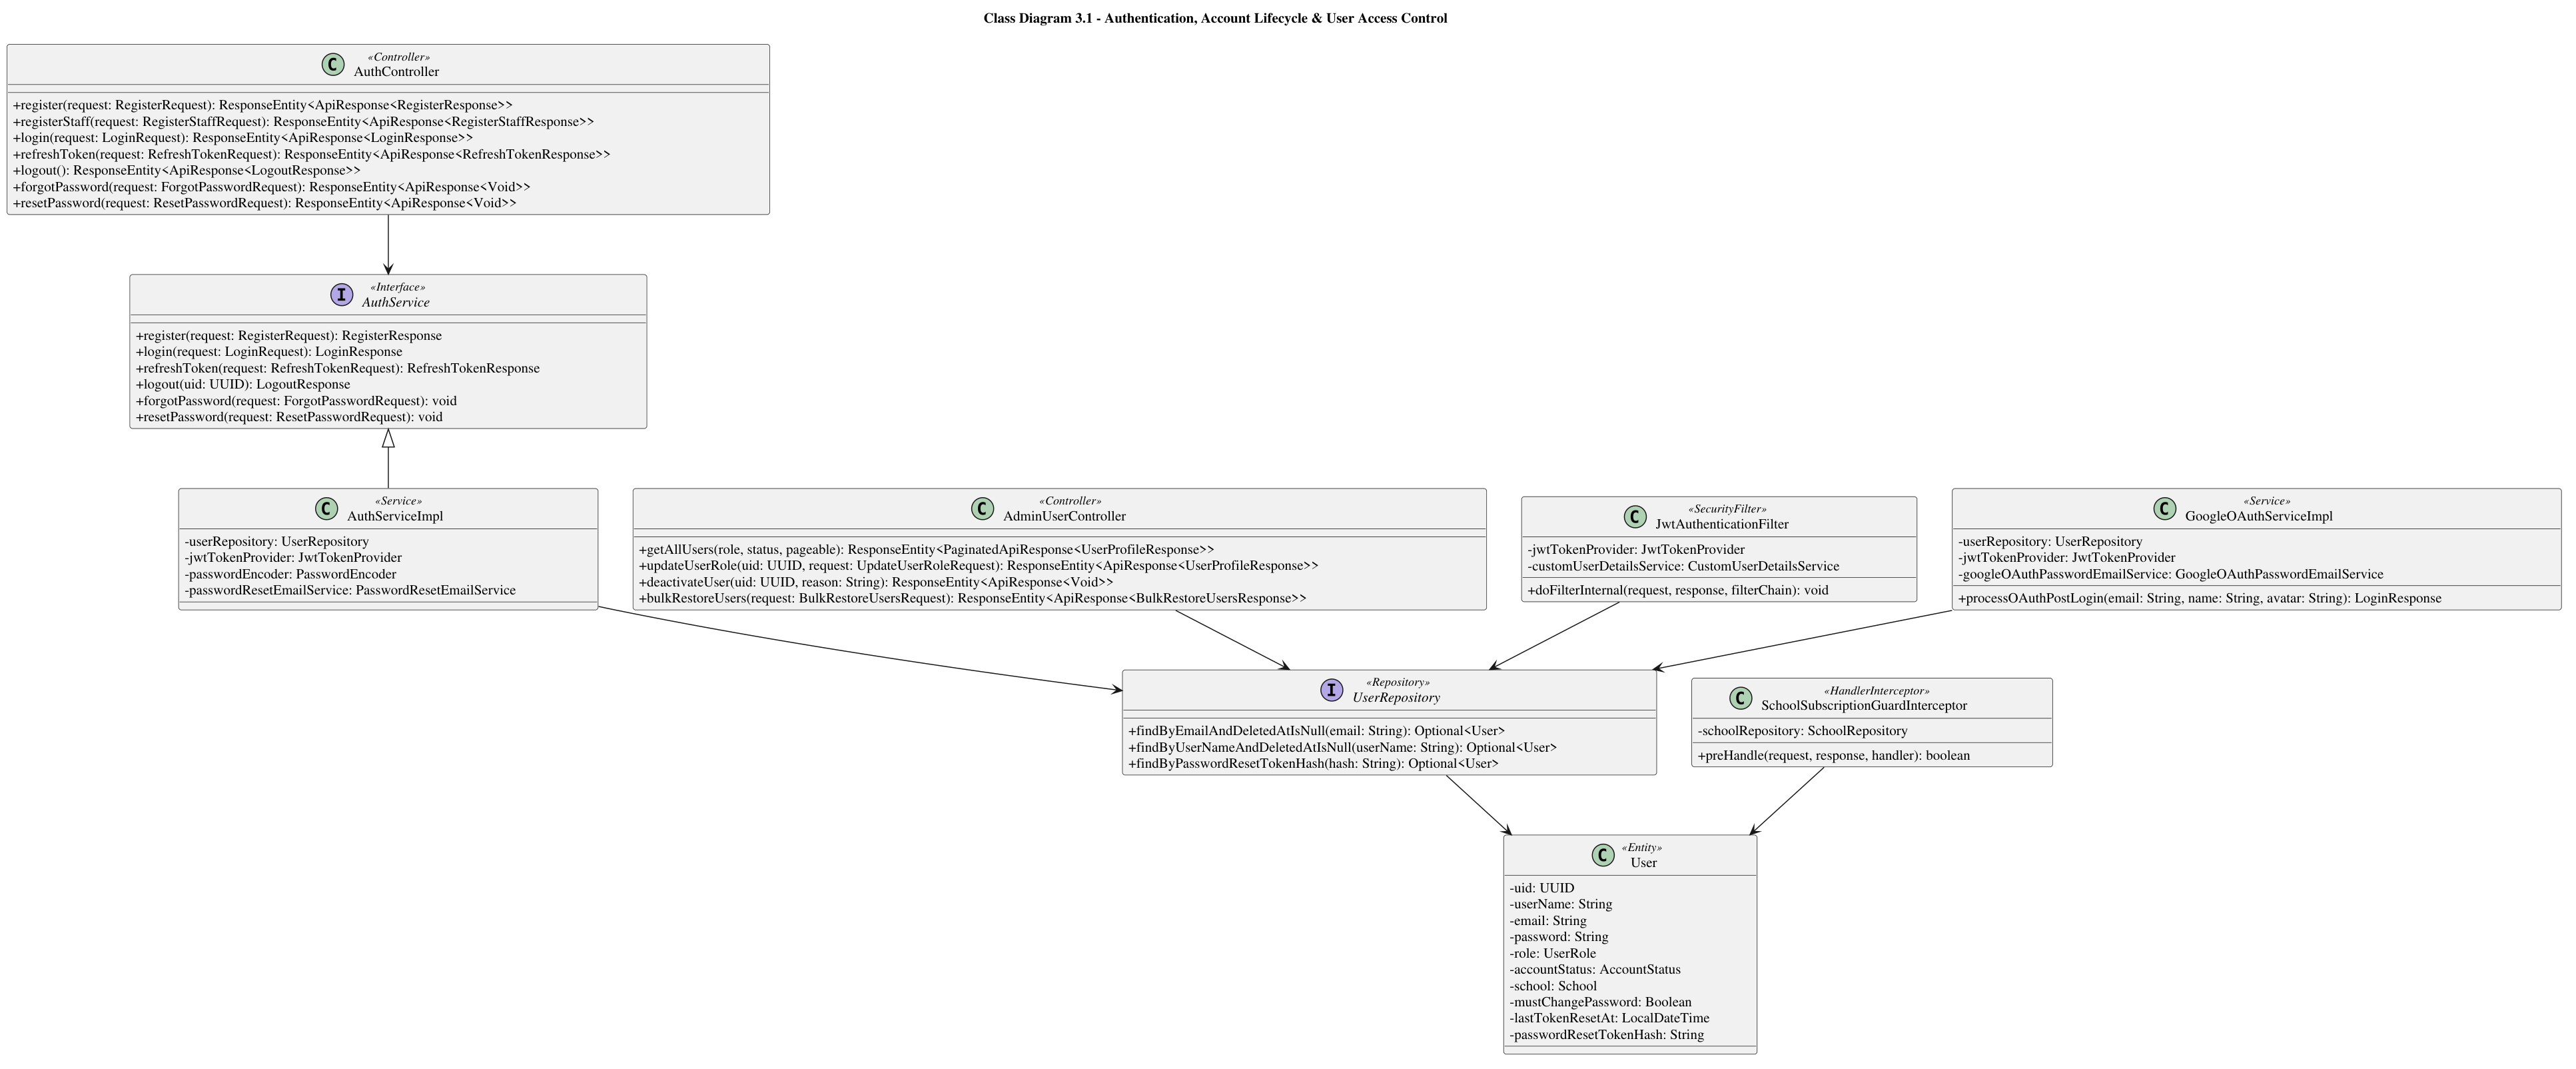
\includegraphics[width=0.98\textwidth]{figures/cls_01_auth_rbac.png}
    \caption{Class Diagram -- Authentication, Account Lifecycle \& Multi-Tenant RBAC}
    \label{fig:cls_01_auth_rbac}
\end{figure}

\begin{longtable}{|L{5.2cm}|L{10.3cm}|}
\hline
\rowcolor{tableheader}
\textbf{Class} & \textbf{Description} \\
\hline
\endhead
\texttt{AuthController} & REST API controller (\texttt{/api/v1/auth}) handling customer registration, staff registration, credential login, JWT refresh token rotation, logout, and forgot/reset password endpoints. \\
\hline
\texttt{AdminUserController} & REST API controller (\texttt{/api/v1/admin/users}) enabling \texttt{SYSTEM\_ADMIN} and \texttt{SCHOOL\_ADMIN} to query paginated user lists, update user roles, deactivate accounts, and bulk-restore soft-deleted users. \\
\hline
\texttt{UserController} & REST API controller (\texttt{/api/v1/users}) managing authenticated user profile retrieval, profile updates, and first-login mandatory password changes (\texttt{mustChangePassword}). \\
\hline
\texttt{JwtAuthenticationFilter} & Spring Security \texttt{OncePerRequestFilter} that extracts Bearer JWT tokens, validates signatures and \texttt{lastTokenResetAt} revocation timestamps, and populates \texttt{SecurityContextHolder}. \\
\hline
\texttt{SchoolSubscriptionGuardInterceptor} & Spring MVC \texttt{HandlerInterceptor} enforcing B2B tenant guards: blocks institutional requests when the user's \texttt{School} is \texttt{SUSPENDED}, \texttt{INACTIVE}, or outside its \texttt{01/09}--\texttt{31/05} subscription window. \\
\hline
\texttt{AuthService} / \texttt{AuthServiceImpl} & Core authentication service interface and implementation managing BCrypt password verification, dual-token issuance, token revocation via \texttt{lastTokenResetAt}, and SHA-256 hashed password reset tokens. \\
\hline
\texttt{GoogleOAuthServiceImpl} & Processes Google OAuth 2.0 SSO callbacks, auto-provisions first-time \texttt{CUSTOMER} accounts with random BCrypt passwords, and dispatches credentials via \texttt{GoogleOAuthPasswordEmailService}. \\
\hline
\texttt{JwtTokenProvider} & Cryptographic utility built on \texttt{jjwt 0.12.5} for signing and parsing access and refresh JWTs containing \texttt{uid}, \texttt{role}, and \texttt{schoolId} claims. \\
\hline
\texttt{UserRepository} & Spring Data JPA repository providing query methods for active/deleted users by email, username, school tenant, and password reset token hash. \\
\hline
\texttt{User} & Core JPA domain entity mapped to \texttt{"user"}, encapsulating identity, 6-role RBAC (\texttt{UserRole}), \texttt{AccountStatus}, B2C/B2B token counters, and audit timestamps. \\
\hline
\caption{Class Descriptions -- Authentication, Account Lifecycle \& Multi-Tenant RBAC}
\label{tab:cls_01_auth_rbac}
\end{longtable}

\subsubsection{Sequence Diagrams: Authentication \& Account Lifecycle}

\begin{figure}[H]
    \centering
    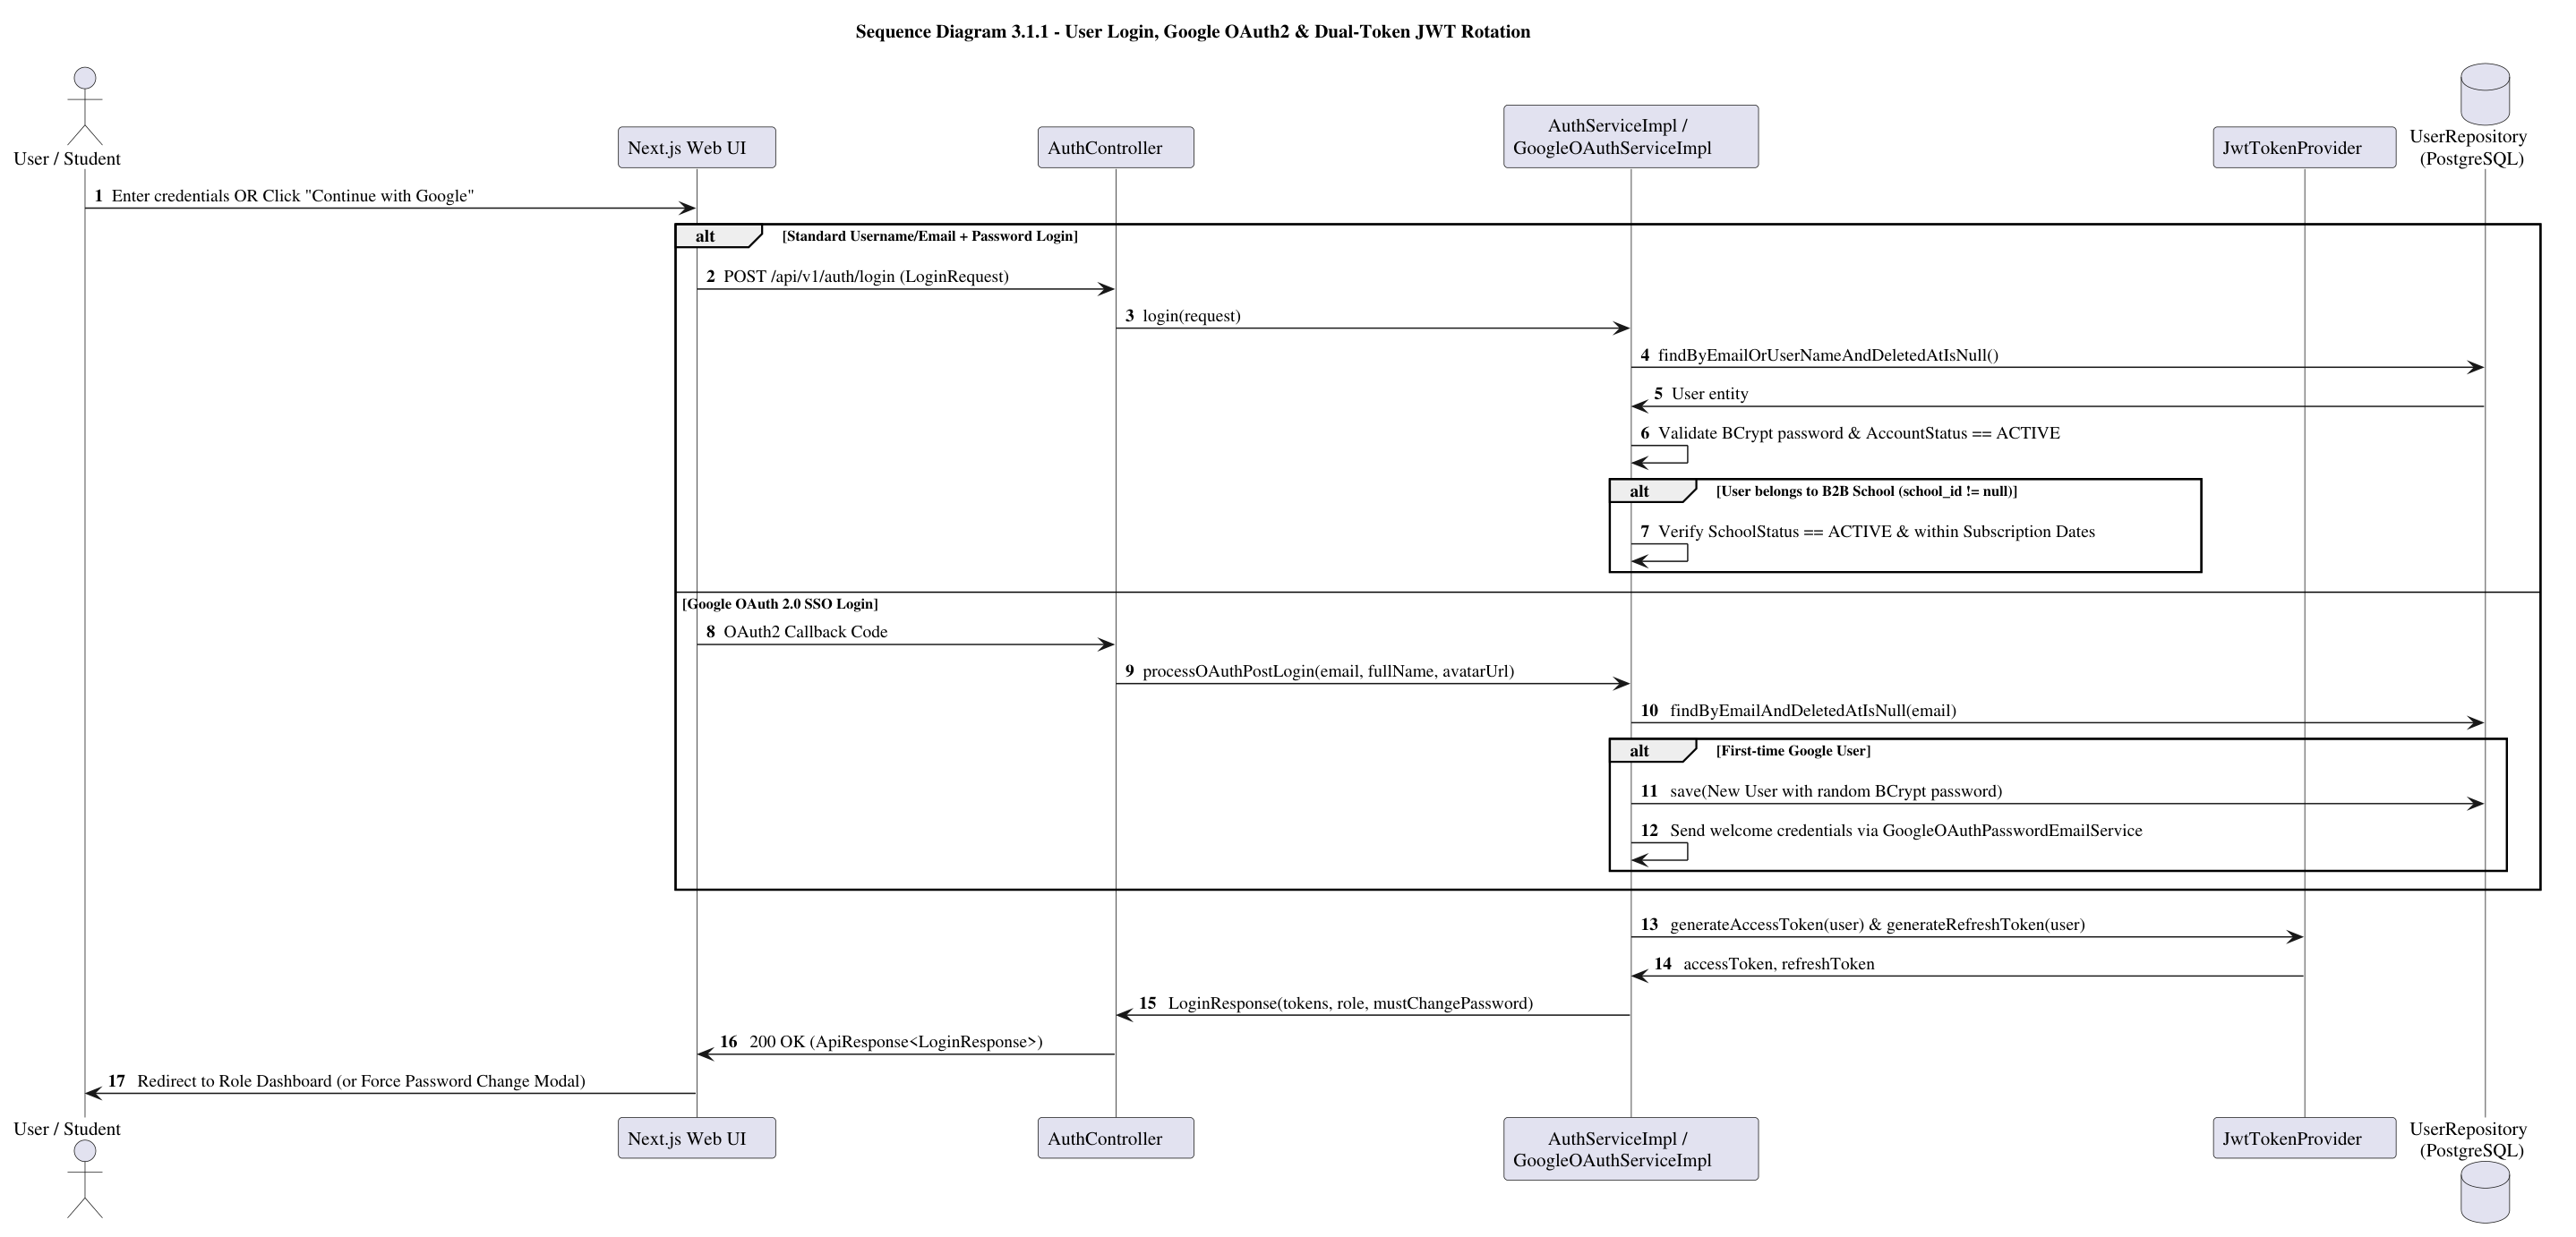
\includegraphics[width=0.98\textwidth]{figures/seq_01_login_oauth_jwt.png}
    \caption{Sequence Diagram -- User Login, Google OAuth2 \& Dual-Token JWT Rotation}
    \label{fig:seq_01_login_oauth_jwt}
\end{figure}

\begin{figure}[H]
    \centering
    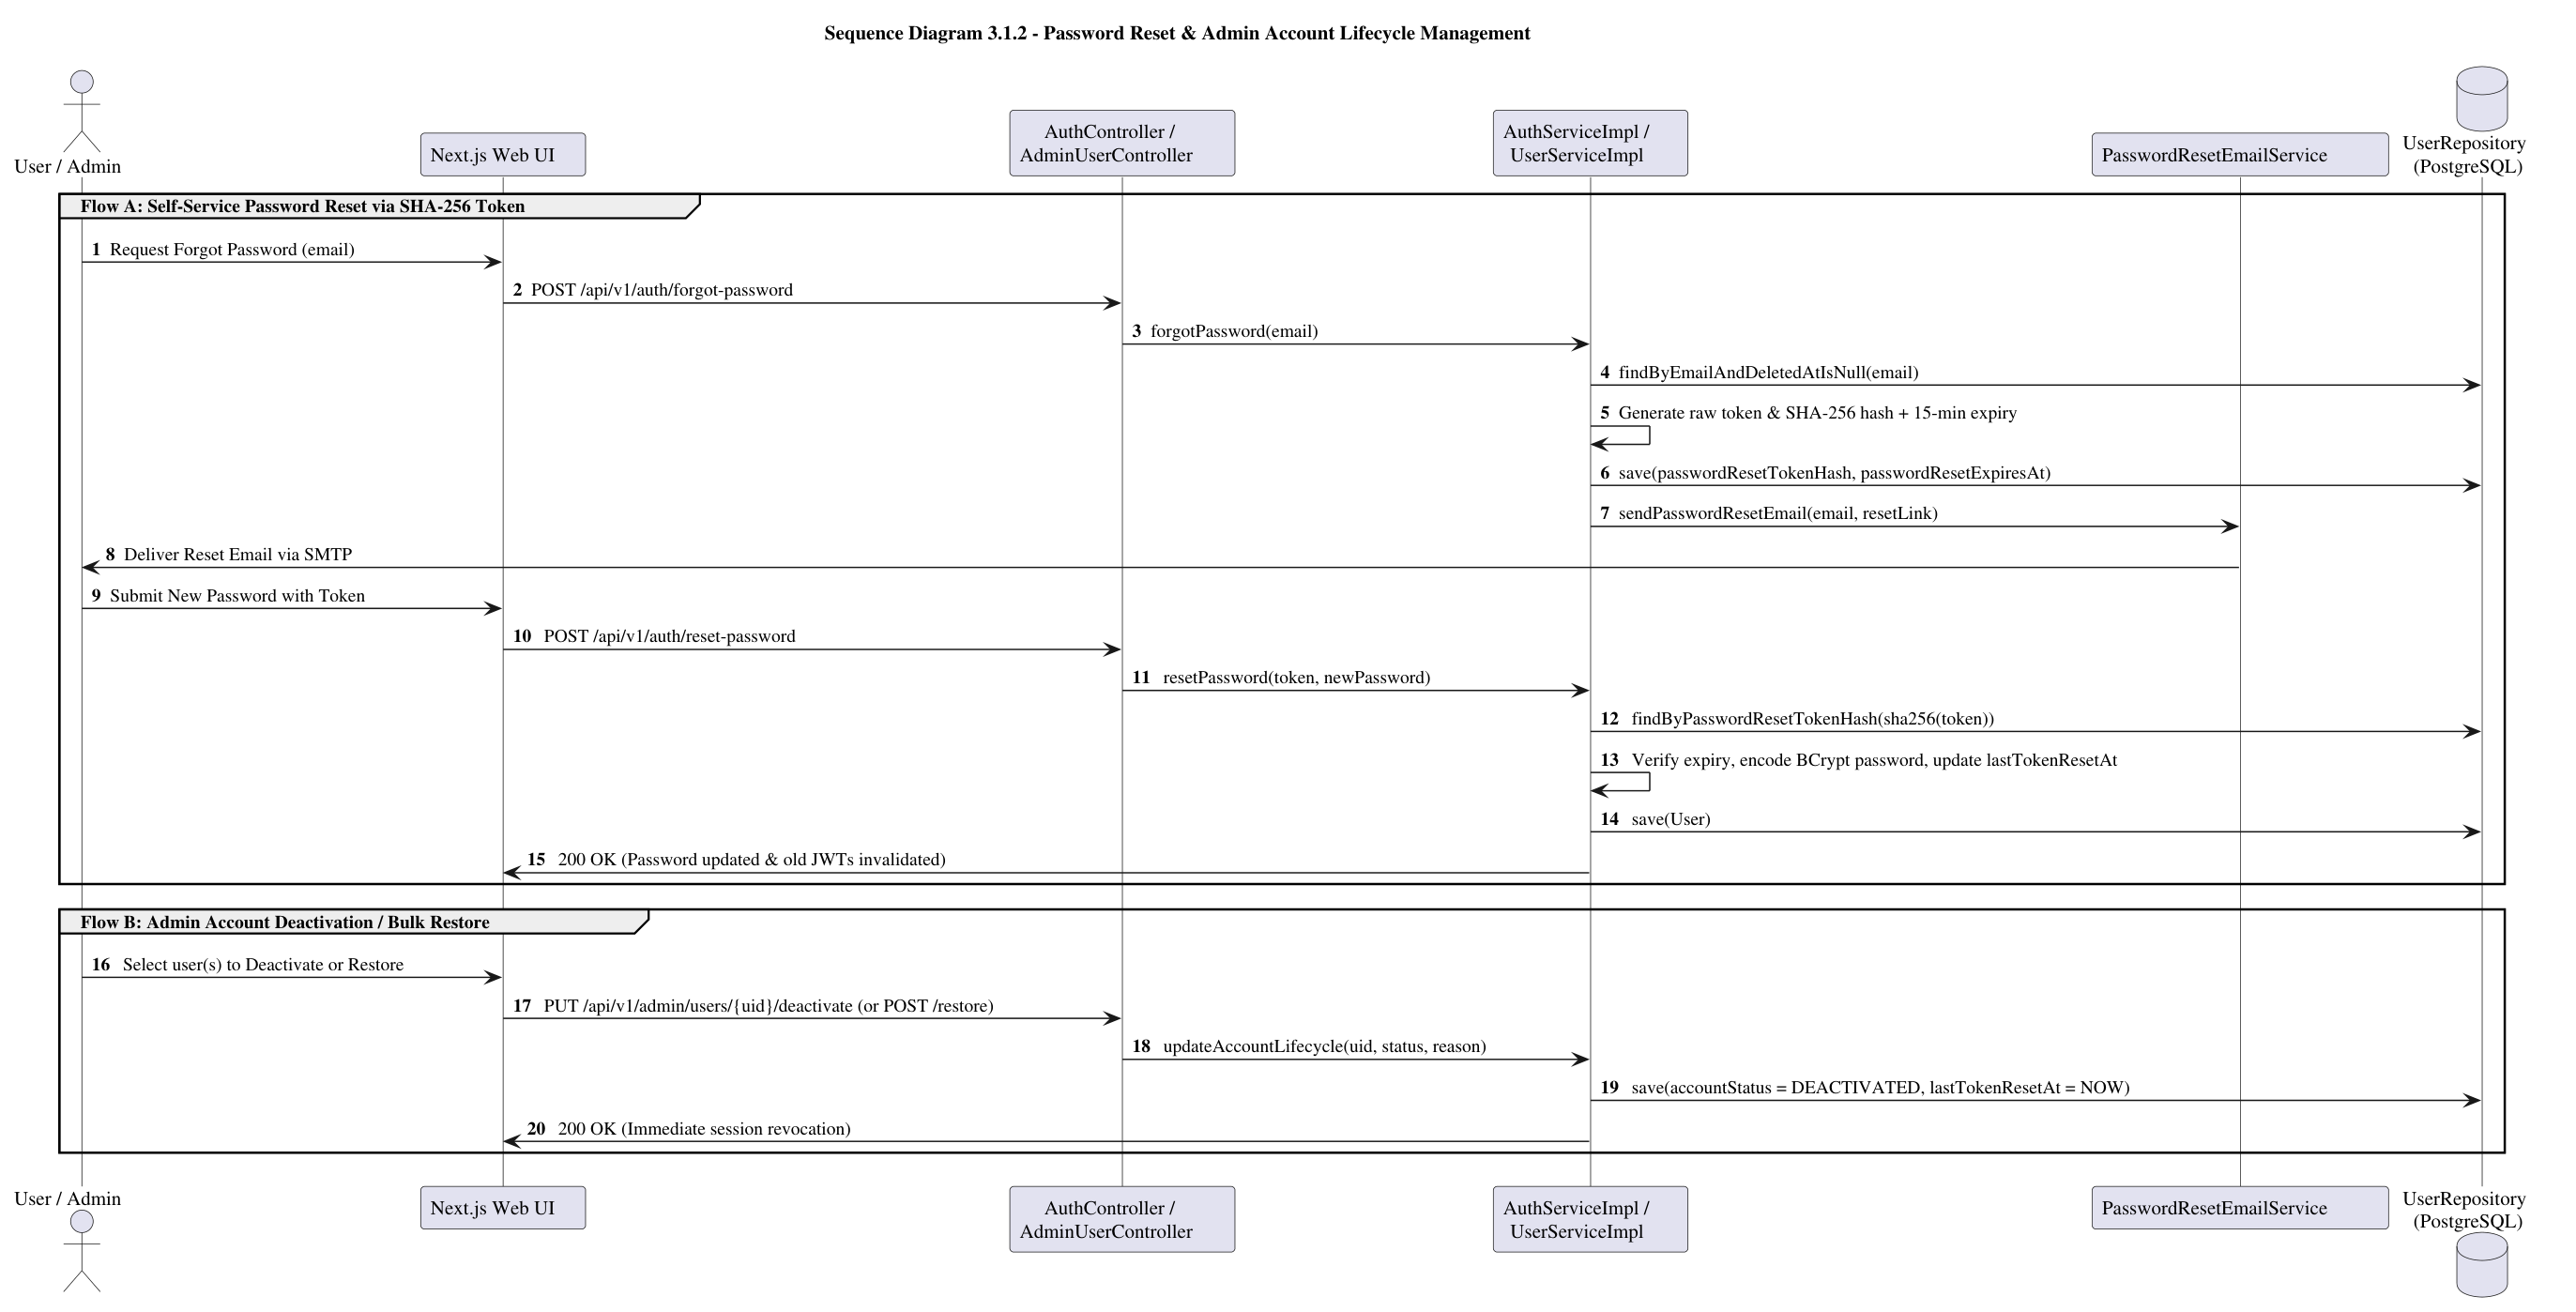
\includegraphics[width=0.98\textwidth]{figures/seq_02_password_reset_and_lifecycle.png}
    \caption{Sequence Diagram -- Self-Service Password Reset \& Admin Account Lifecycle Management}
    \label{fig:seq_02_password_reset_and_lifecycle}
\end{figure}

\newpage
\subsection{B2B SaaS School, Classroom \& Token Quota Allocation}

\subsubsection{Class Diagram: B2B SaaS School, Classroom \& Token Quota Allocation}

\begin{figure}[H]
    \centering
    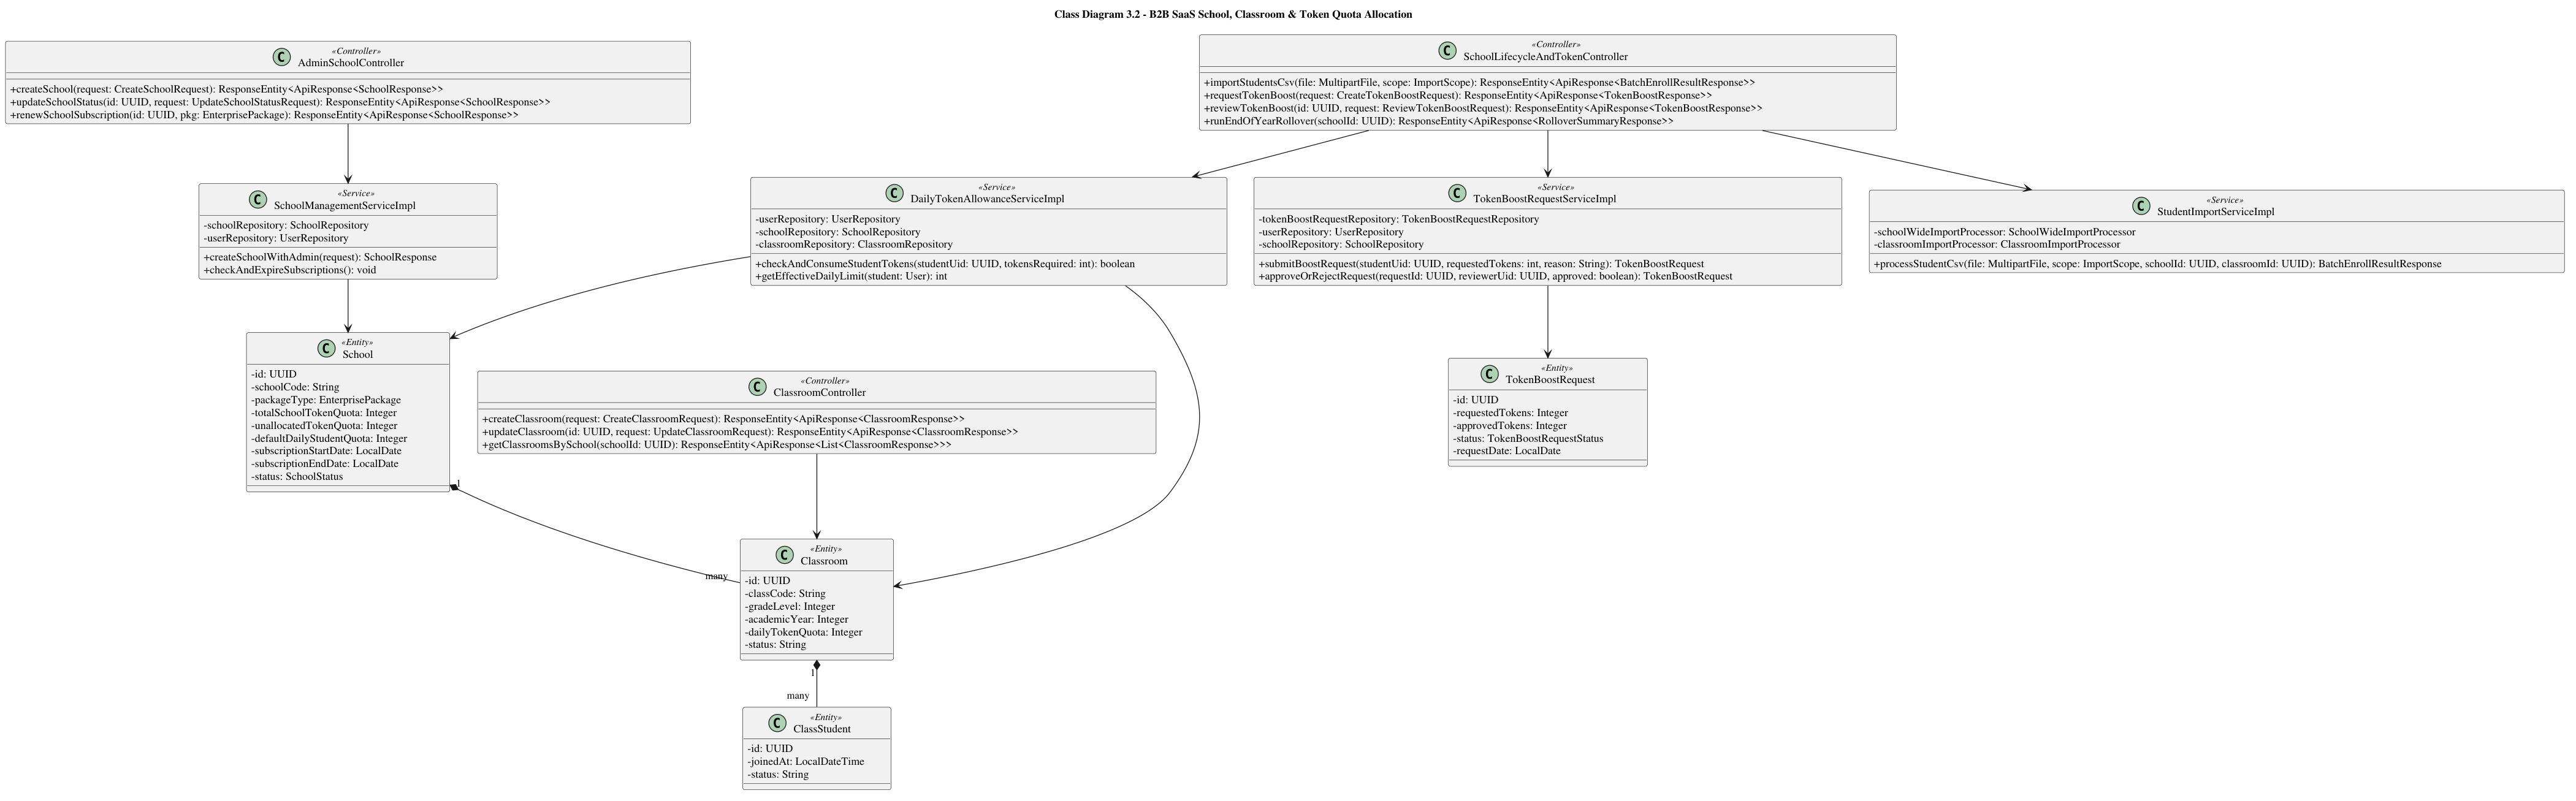
\includegraphics[width=0.98\textwidth]{figures/cls_02_school_classroom_token.png}
    \caption{Class Diagram -- B2B SaaS School, Classroom \& Token Quota Allocation}
    \label{fig:cls_02_school_classroom_token}
\end{figure}

\begin{longtable}{|L{5.5cm}|L{10.0cm}|}
\hline
\rowcolor{tableheader}
\textbf{Class} & \textbf{Description} \\
\hline
\endhead
\texttt{AdminSchoolController} & REST API controller (\texttt{/api/v1/admin/schools}) for \texttt{SYSTEM\_ADMIN} to provision B2B school tenants, assign \texttt{EnterprisePackage} tiers, and manage school subscription statuses. \\
\hline
\texttt{ClassroomController} / \texttt{ClassroomStudentController} & REST API controllers managing school classrooms, teacher assignments, student roster listings, classroom transfers, and smart class join codes (\texttt{SmartClassCodeGenerator}). \\
\hline
\texttt{SchoolLifecycleAndTokenController} & REST API controller (\texttt{/api/v1/schools}) handling bulk CSV student imports, daily token boost requests/approvals, and end-of-academic-year student lifecycle rollovers. \\
\hline
\texttt{SchoolManagementServiceImpl} & Manages school creation, initial \texttt{SCHOOL\_ADMIN} provisioning, enterprise token pool initialization, and scheduled subscription expiration checks. \\
\hline
\texttt{AcademicLifecycleServiceImpl} & Executes end-of-year academic promotions: promotes Grade 6--11 classrooms, archives completed cohorts, and transitions graduating Grade 12 student accounts to \texttt{DEACTIVATED}. \\
\hline
\texttt{StudentImportServiceImpl} & Coordinates \texttt{SchoolWideImportProcessor} and \texttt{ClassroomImportProcessor} using \texttt{Apache Commons CSV} to batch-create student accounts and auto-exempt past-deadline classroom assignments. \\
\hline
\texttt{DailyTokenAllowanceServiceImpl} & Enforces B2B student daily token limits with lazy midnight resets, resolving effective limits from classroom overrides or school defaults plus approved daily bonus tokens. \\
\hline
\texttt{TokenBoostRequestServiceImpl} & Manages the student daily token boost lifecycle (\texttt{PENDING} $\rightarrow$ \texttt{APPROVED}/\texttt{REJECTED}), deducting approved tokens from the school's shared \texttt{unallocatedTokenQuota}. \\
\hline
\texttt{School}, \texttt{Classroom}, \texttt{ClassStudent}, \texttt{TokenBoostRequest} & Persistent JPA domain entities modeling the multi-tenant school hierarchy, classroom rosters, and daily token boost requests. \\
\hline
\caption{Class Descriptions -- B2B SaaS School, Classroom \& Token Quota Allocation}
\label{tab:cls_02_school_classroom_token}
\end{longtable}

\subsubsection{Sequence Diagrams: School Provisioning, CSV Import \& Token Boost}

\begin{figure}[H]
    \centering
    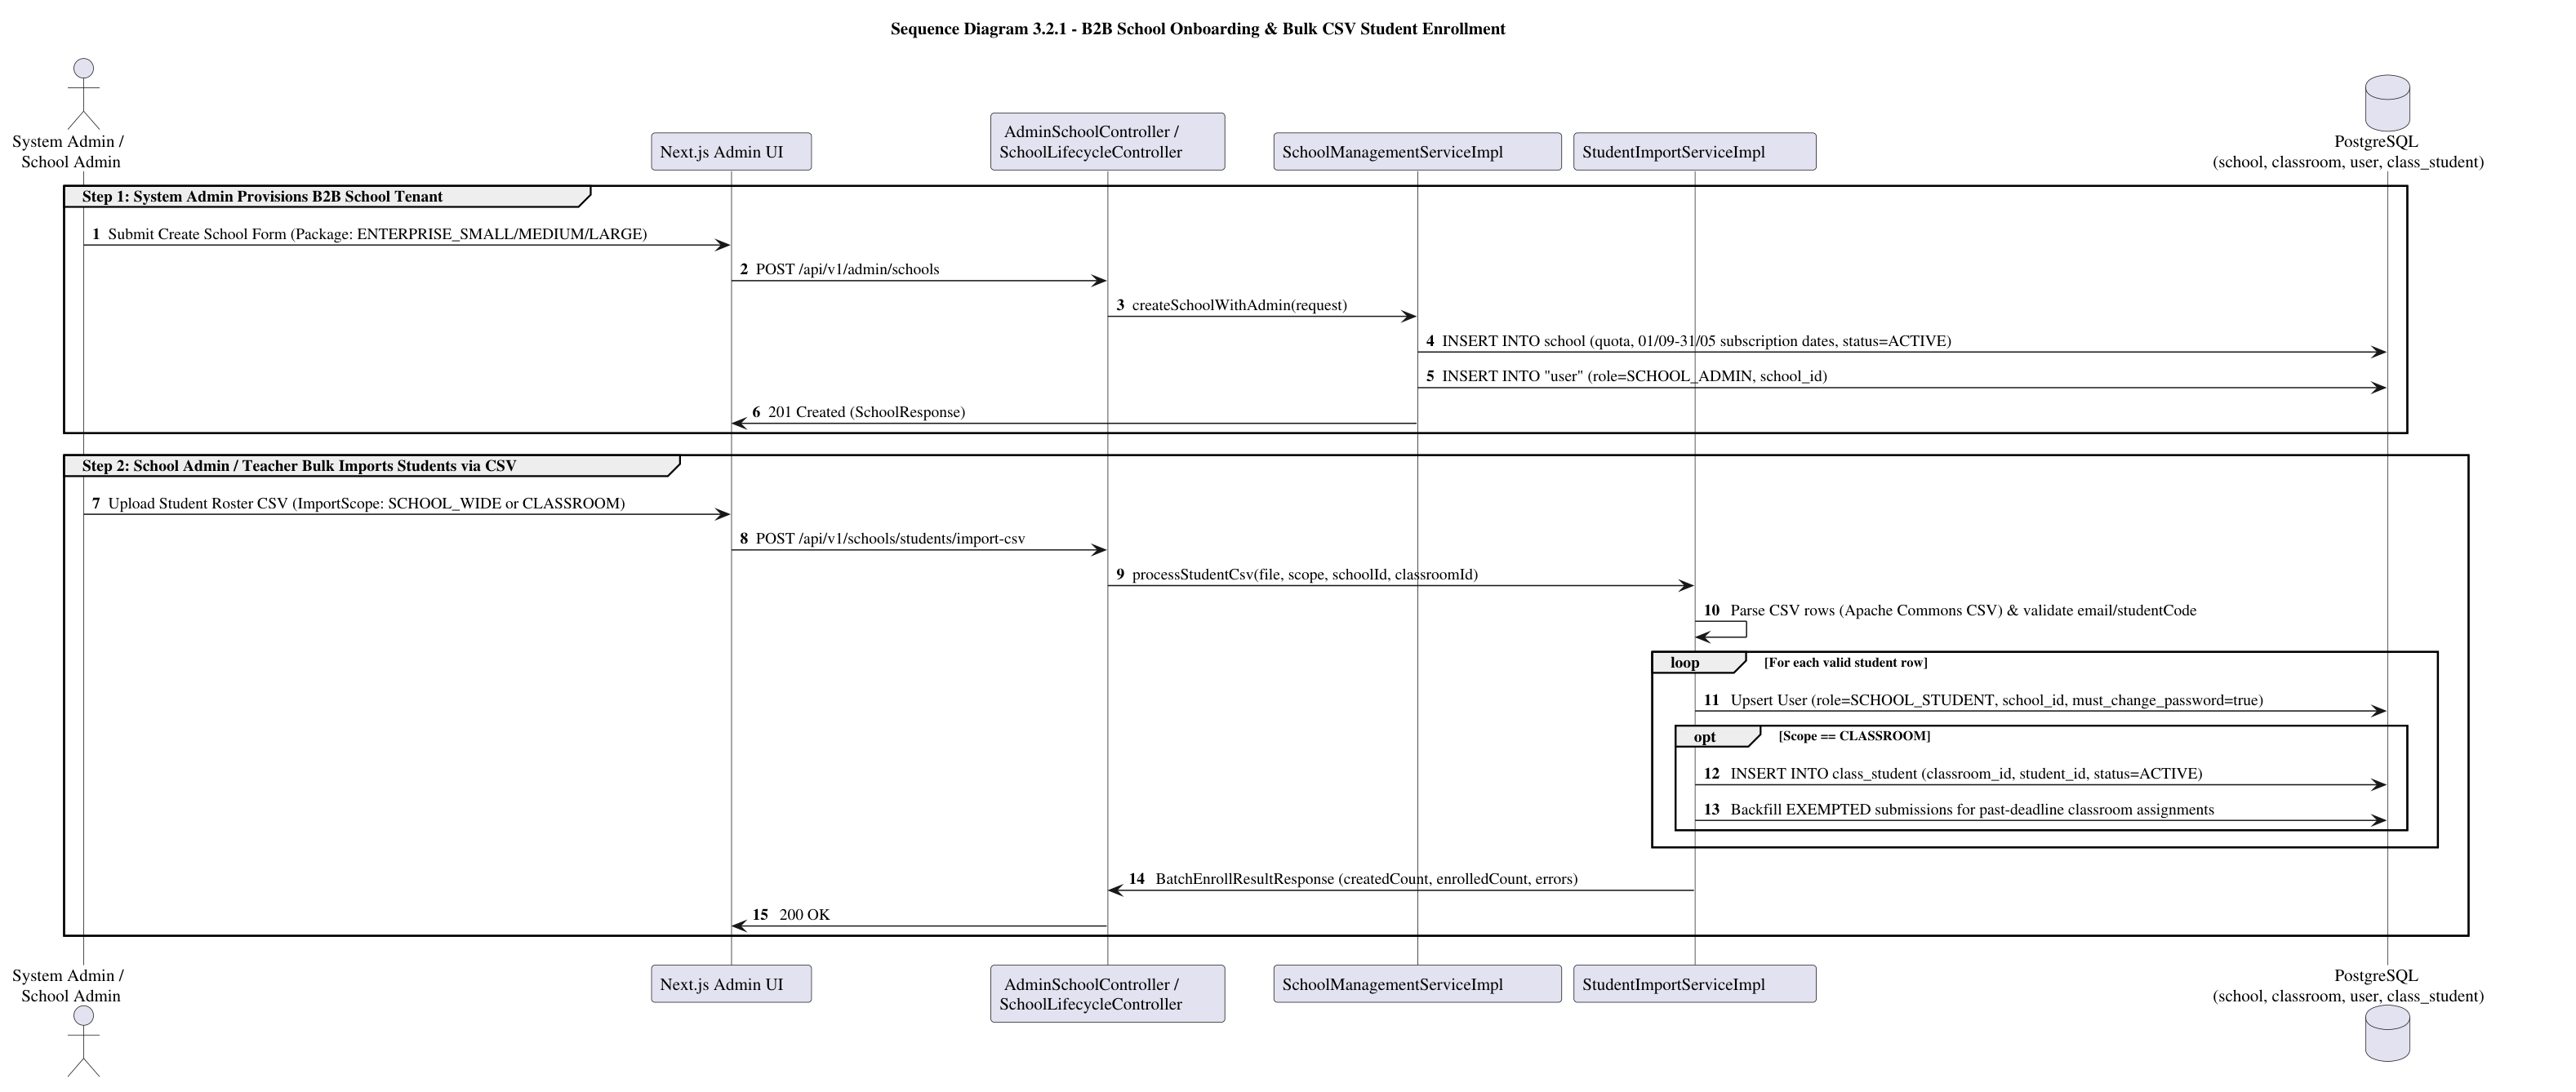
\includegraphics[width=0.98\textwidth]{figures/seq_03_school_provisioning_and_import.png}
    \caption{Sequence Diagram -- B2B School Onboarding \& Bulk CSV Student Enrollment}
    \label{fig:seq_03_school_provisioning_and_import}
\end{figure}

\begin{figure}[H]
    \centering
    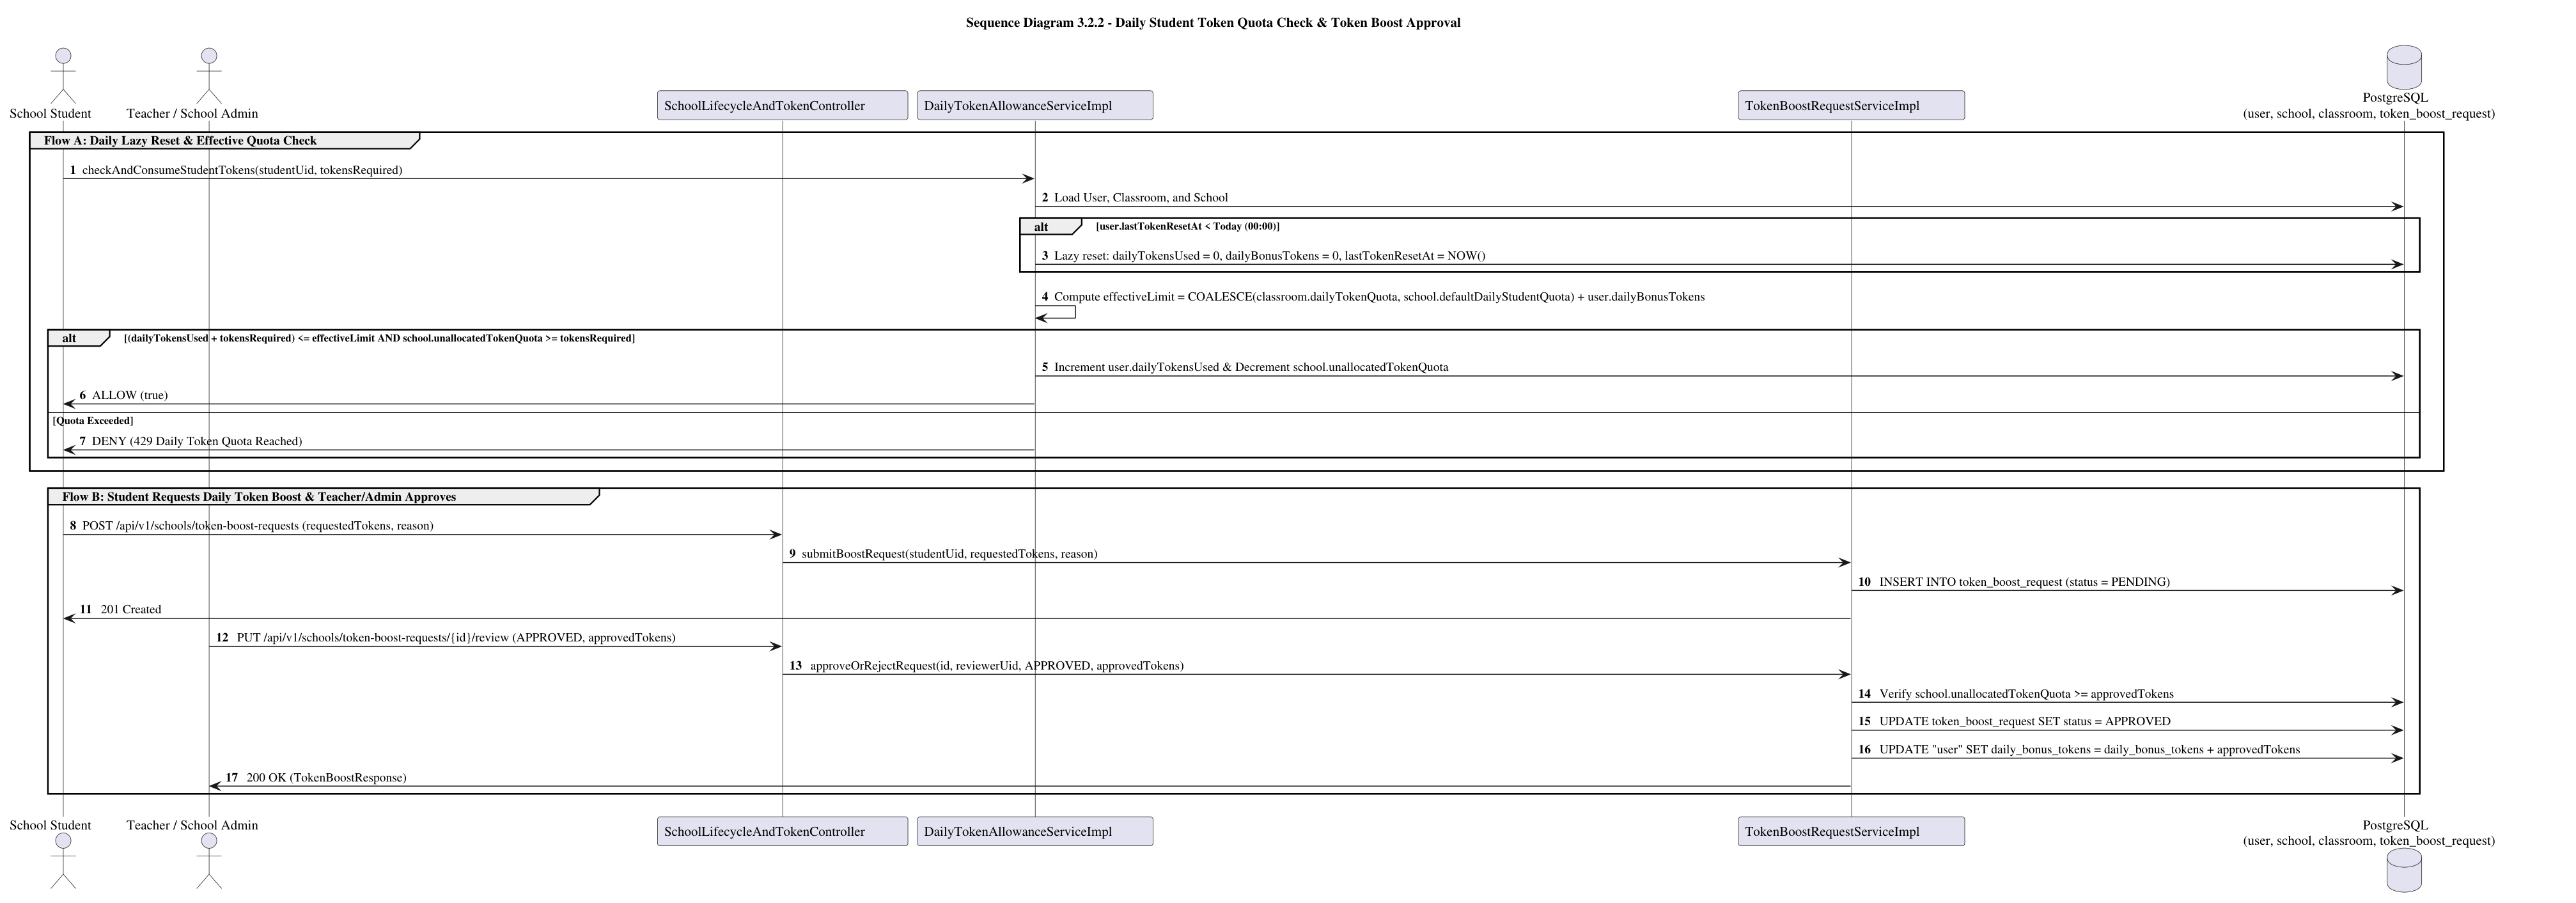
\includegraphics[width=0.98\textwidth]{figures/seq_04_token_boost_and_allowance.png}
    \caption{Sequence Diagram -- Daily Student Token Quota Check \& Token Boost Request Approval}
    \label{fig:seq_04_token_boost_and_allowance}
\end{figure}

\newpage
\subsection{Historical Content, Character, Document OCR \& Interactive Map}

\subsubsection{Class Diagram: Historical Content, Character, Document OCR \& Interactive Map}

\begin{figure}[H]
    \centering
    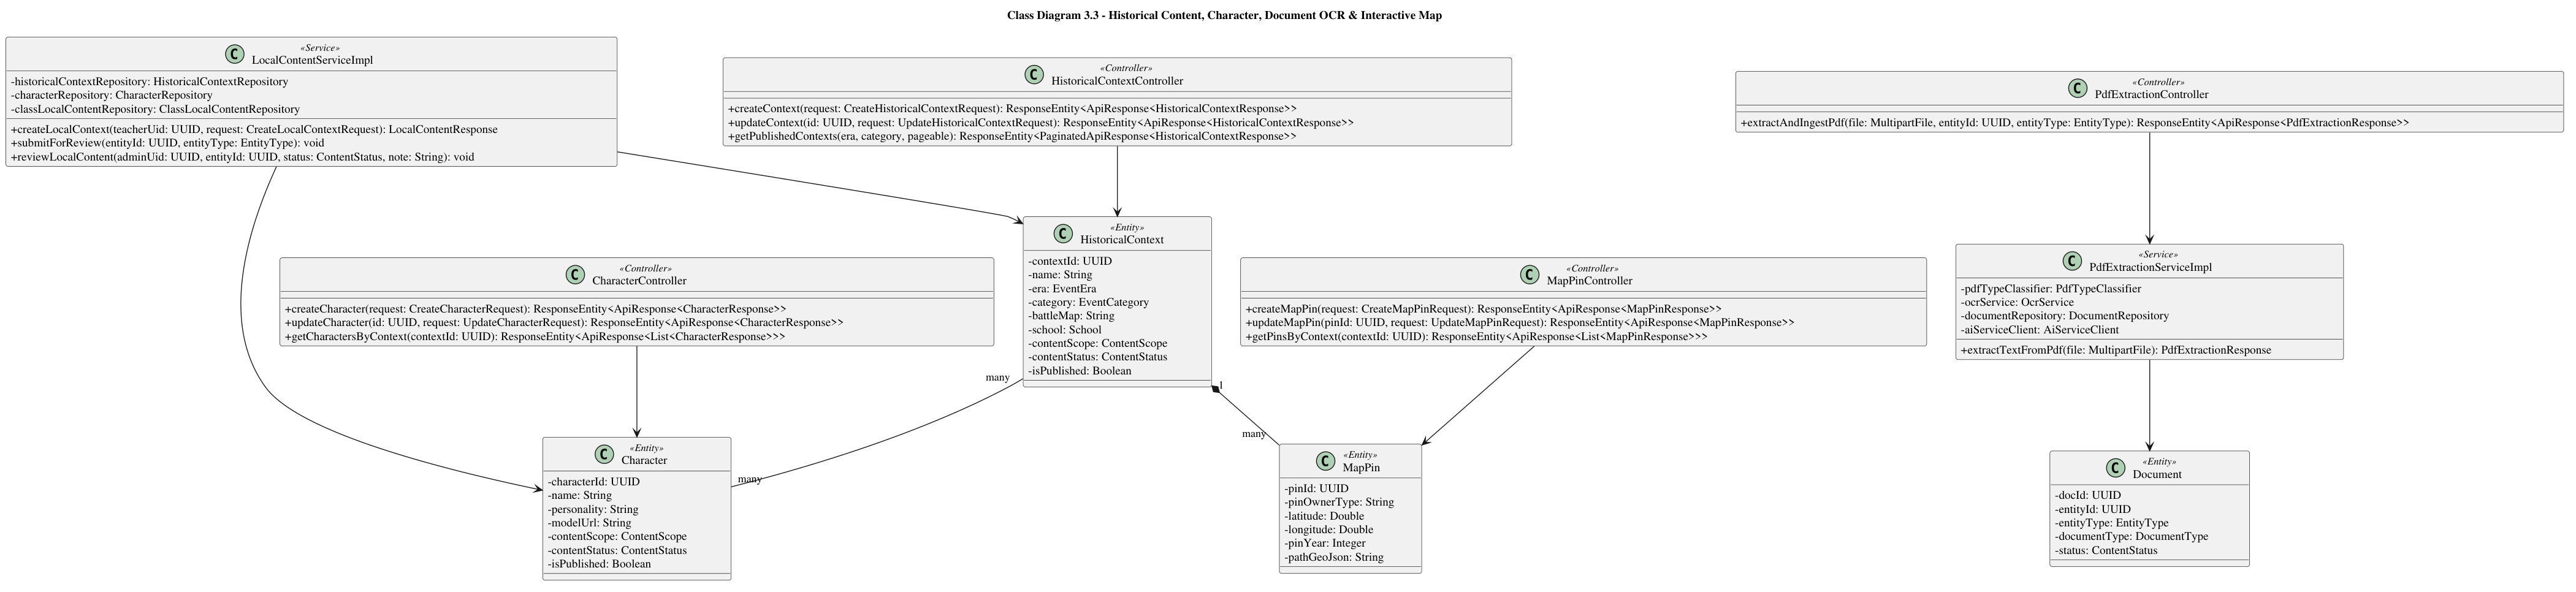
\includegraphics[width=0.98\textwidth]{figures/cls_03_content_character_map.png}
    \caption{Class Diagram -- Historical Content, Character, Document OCR \& Interactive Map}
    \label{fig:cls_03_content_character_map}
\end{figure}

\begin{longtable}{|L{5.5cm}|L{10.0cm}|}
\hline
\rowcolor{tableheader}
\textbf{Class} & \textbf{Description} \\
\hline
\endhead
\texttt{HistoricalContextController} & REST API controller (\texttt{/api/v1/historical-contexts}) providing CRUD, publication toggling, and filtered timeline pagination by \texttt{EventEra} and \texttt{EventCategory}. \\
\hline
\texttt{CharacterController} & REST API controller (\texttt{/api/v1/characters}) managing historical character biographies, persona prompts, 3D model URLs, and context associations. \\
\hline
\texttt{PdfExtractionController} / \texttt{DocumentFileController} & REST API controllers handling PDF upload, automatic text/OCR extraction, document persistence, and asynchronous RAG vector indexing triggers. \\
\hline
\texttt{MapPinController} / \texttt{MapFocusController} & REST API controllers managing GeoJSON battle-map pins (\texttt{ADMIN} and \texttt{USER} pins), troop movement \texttt{LineString} paths, and camera viewpoint focuses. \\
\hline
\texttt{TeacherLocalContentController} / \texttt{SchoolAdminLocalContentController} & REST API controllers enabling teachers to author local history contexts/characters and school admins to review and approve/reject them (\texttt{PENDING\_REVIEW} $\rightarrow$ \texttt{ACTIVE}/\texttt{DRAFT}). \\
\hline
\texttt{PdfExtractionServiceImpl} / \texttt{OcrServiceImpl} & Classifies uploaded PDFs via \texttt{PdfTypeClassifier}; extracts digital text via \texttt{Apache PDFBox 3.0.1} or falls back to \texttt{Tess4J 5.10.0} Vietnamese OCR (\texttt{vie.traineddata}) for scanned historical archives. \\
\hline
\texttt{LocalContentServiceImpl} & Enforces multi-tenant isolation and policy checks (\texttt{localHistoryPolicyAccepted}) for school-owned local historical content and classroom assignments (\texttt{ClassLocalContent}). \\
\hline
\texttt{HistoricalContext}, \texttt{Character}, \texttt{Document}, \texttt{MapPin}, \texttt{MapFocus} & Domain entities representing historical events, roleplay personas, RAG source documents, and interactive GeoJSON map elements. \\
\hline
\caption{Class Descriptions -- Historical Content, Character, Document OCR \& Interactive Map}
\label{tab:cls_03_content_character_map}
\end{longtable}

\subsubsection{Sequence Diagrams: PDF OCR Ingestion \& Local Content Approval}

\begin{figure}[H]
    \centering
    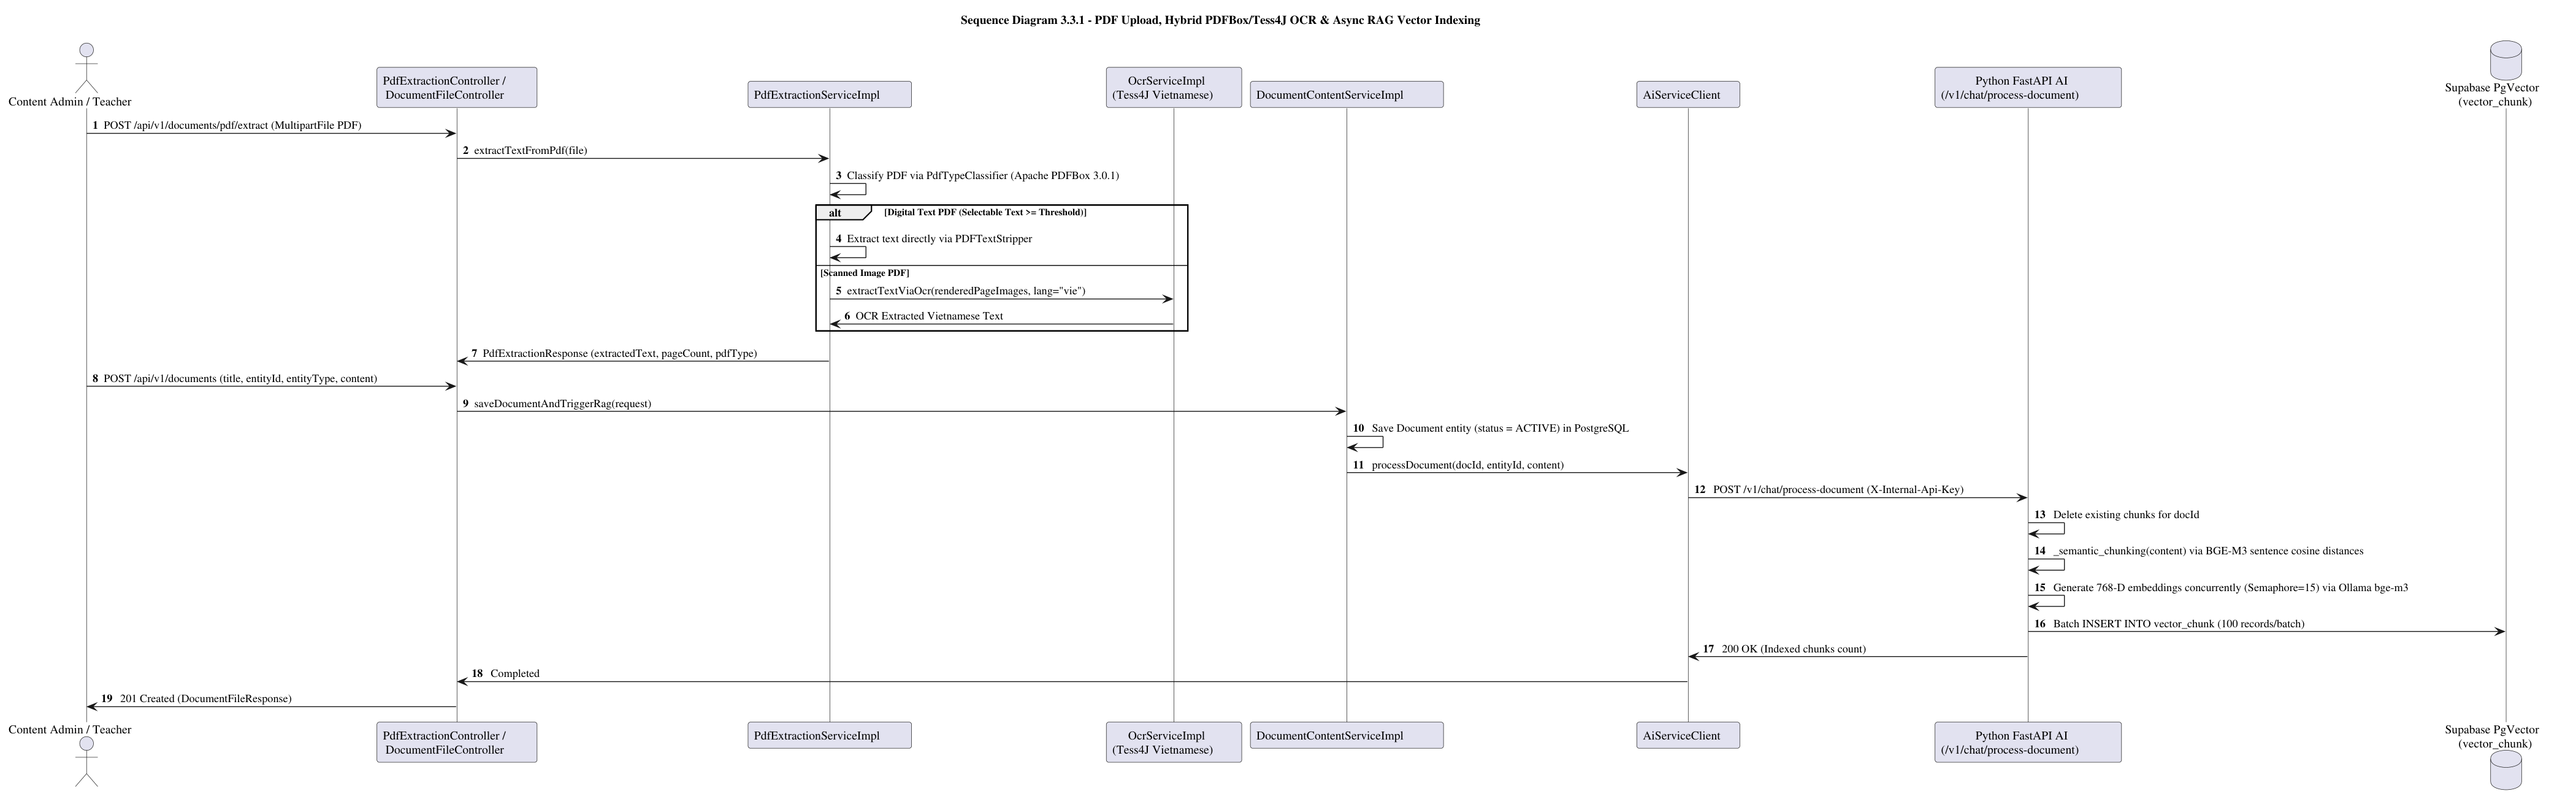
\includegraphics[width=0.98\textwidth]{figures/seq_05_document_ocr_and_rag_sync.png}
    \caption{Sequence Diagram -- PDF Upload, Hybrid PDFBox/Tess4J OCR \& Async RAG Vector Indexing}
    \label{fig:seq_05_document_ocr_and_rag_sync}
\end{figure}

\begin{figure}[H]
    \centering
    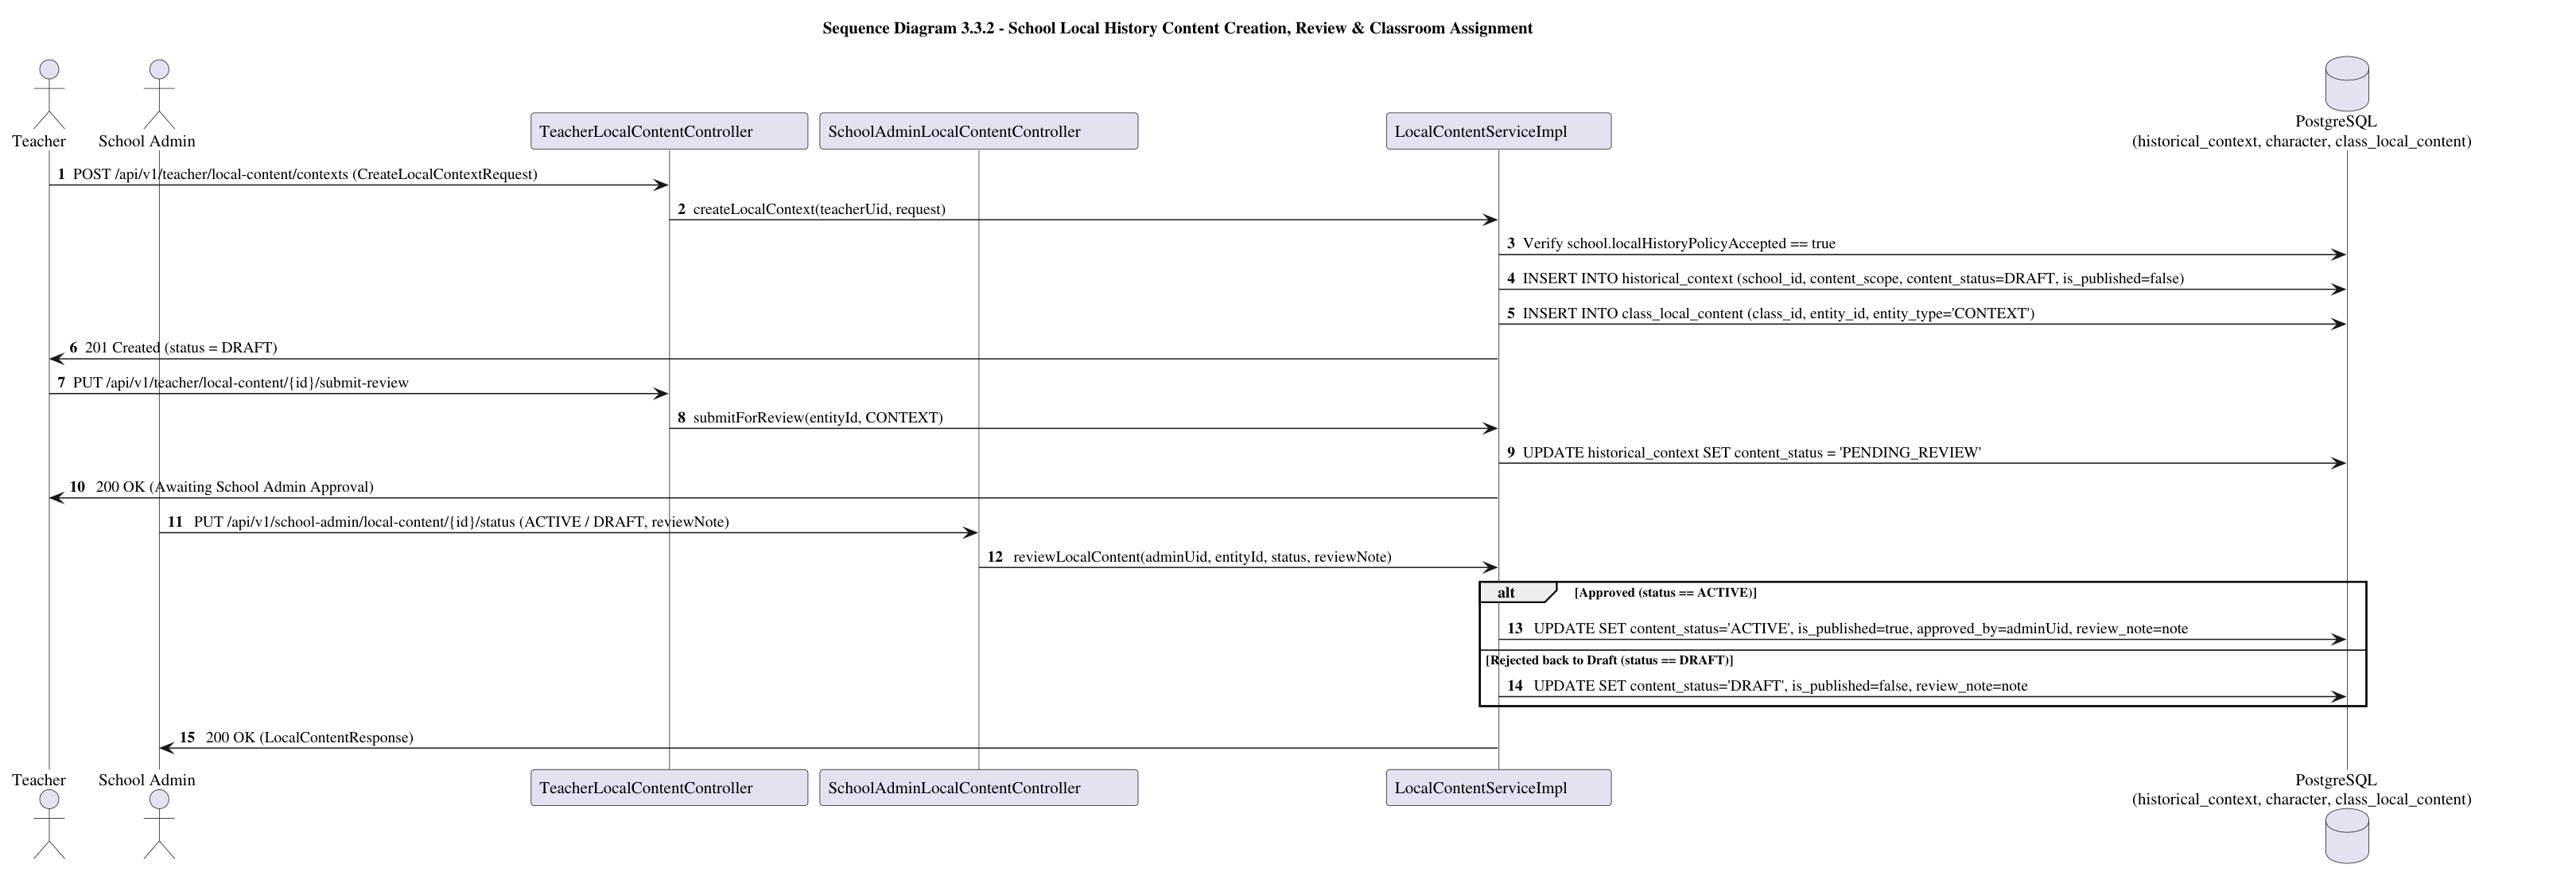
\includegraphics[width=0.98\textwidth]{figures/seq_06_local_content_approval.png}
    \caption{Sequence Diagram -- School Local History Content Creation, Review \& Classroom Assignment}
    \label{fig:seq_06_local_content_approval}
\end{figure}

\newpage
\subsection{Conversational AI Roleplay \& Hybrid RAG Microservice}

\subsubsection{Class Diagram: Conversational AI Roleplay \& Hybrid RAG Microservice}

\begin{figure}[H]
    \centering
    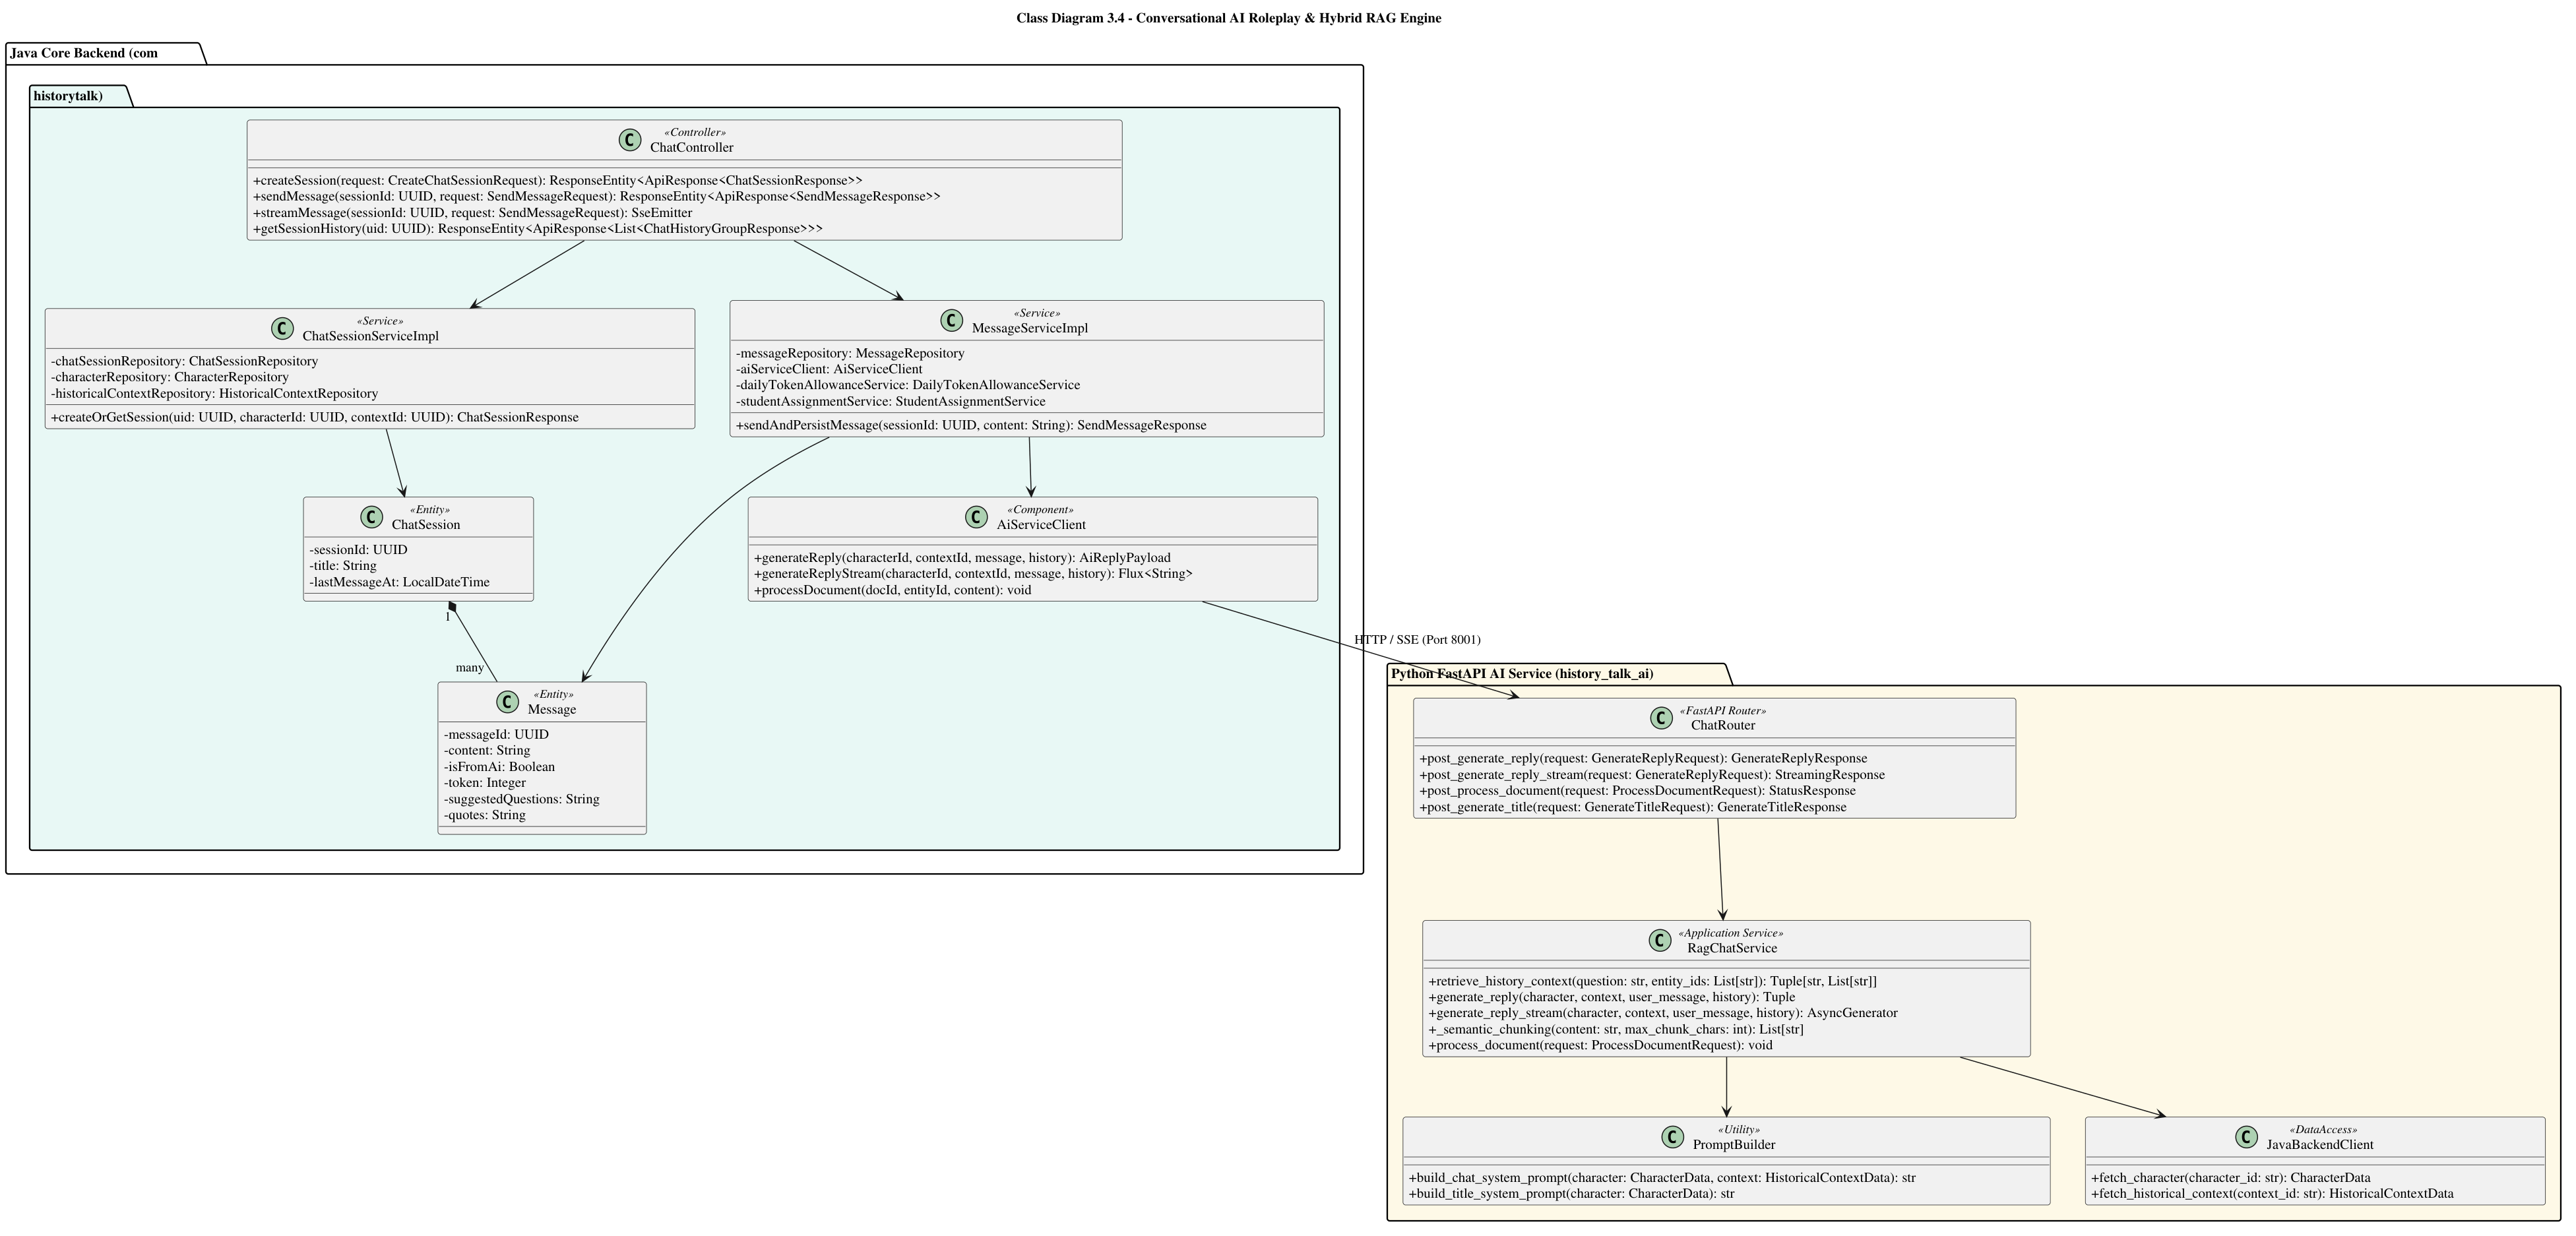
\includegraphics[width=0.98\textwidth]{figures/cls_04_chat_and_ai_rag.png}
    \caption{Class Diagram -- Conversational AI Roleplay \& Hybrid RAG Microservice}
    \label{fig:cls_04_chat_and_ai_rag}
\end{figure}

\begin{longtable}{|L{5.5cm}|L{10.0cm}|}
\hline
\rowcolor{tableheader}
\textbf{Class} & \textbf{Description} \\
\hline
\endhead
\texttt{ChatController} (Java) & Exposes endpoints (\texttt{/api/v1/chat}) for creating chat sessions, retrieving grouped conversation history, and streaming AI character responses over SSE. \\
\hline
\texttt{ChatSessionServiceImpl} (Java) & Manages chat session lifecycles, initial character greeting generation, and automatic short session title updates after the first dialogue exchange. \\
\hline
\texttt{MessageServiceImpl} (Java) & Coordinates token quota verification, user message persistence, AI microservice invocation, AI message persistence, and automatic \texttt{AI\_CHAT\_ROLEPLAY} assignment progress tracking. \\
\hline
\texttt{AiServiceClient} (Java) & HTTP/SSE integration client communicating with the Python FastAPI microservice using \texttt{X-Internal-Api-Key} authentication and Micrometer latency metrics (\texttt{AiMetricsService}). \\
\hline
\texttt{ChatRouter} (Python FastAPI) & Presentation router (\texttt{presentation/chat/router.py}) exposing \texttt{/v1/chat/generate-reply}, \texttt{/generate-reply-stream}, \texttt{/generate-title}, and \texttt{/process-document}. \\
\hline
\texttt{RagChatService} (Python FastAPI) & Core RAG module (\texttt{application/chat/service.py}) implementing dynamic 80th-percentile semantic chunking, \texttt{bge-m3} embedding generation, Supabase \texttt{match\_history\_chunks} RPC retrieval, Kaggle cross-encoder reranking, and streaming LLM roleplay. \\
\hline
\texttt{PromptBuilder} (Python FastAPI) & Constructs 1st-person historical persona system prompts (\texttt{prompt\_builder.py}), enforcing anti-hallucination guardrails and a 30\% probability Socratic reverse-questioning directive. \\
\hline
\texttt{JavaBackendClient} (Python FastAPI) & Asynchronous \texttt{httpx} data access client (\texttt{dataaccess/java\_backend/client.py}) fetching character profiles and context metadata from the Java backend. \\
\hline
\caption{Class Descriptions -- Conversational AI Roleplay \& Hybrid RAG Microservice}
\label{tab:cls_04_chat_and_ai_rag}
\end{longtable}

\subsubsection{Sequence Diagram: Streaming Conversational AI Roleplay with Hybrid RAG}

\begin{figure}[H]
    \centering
    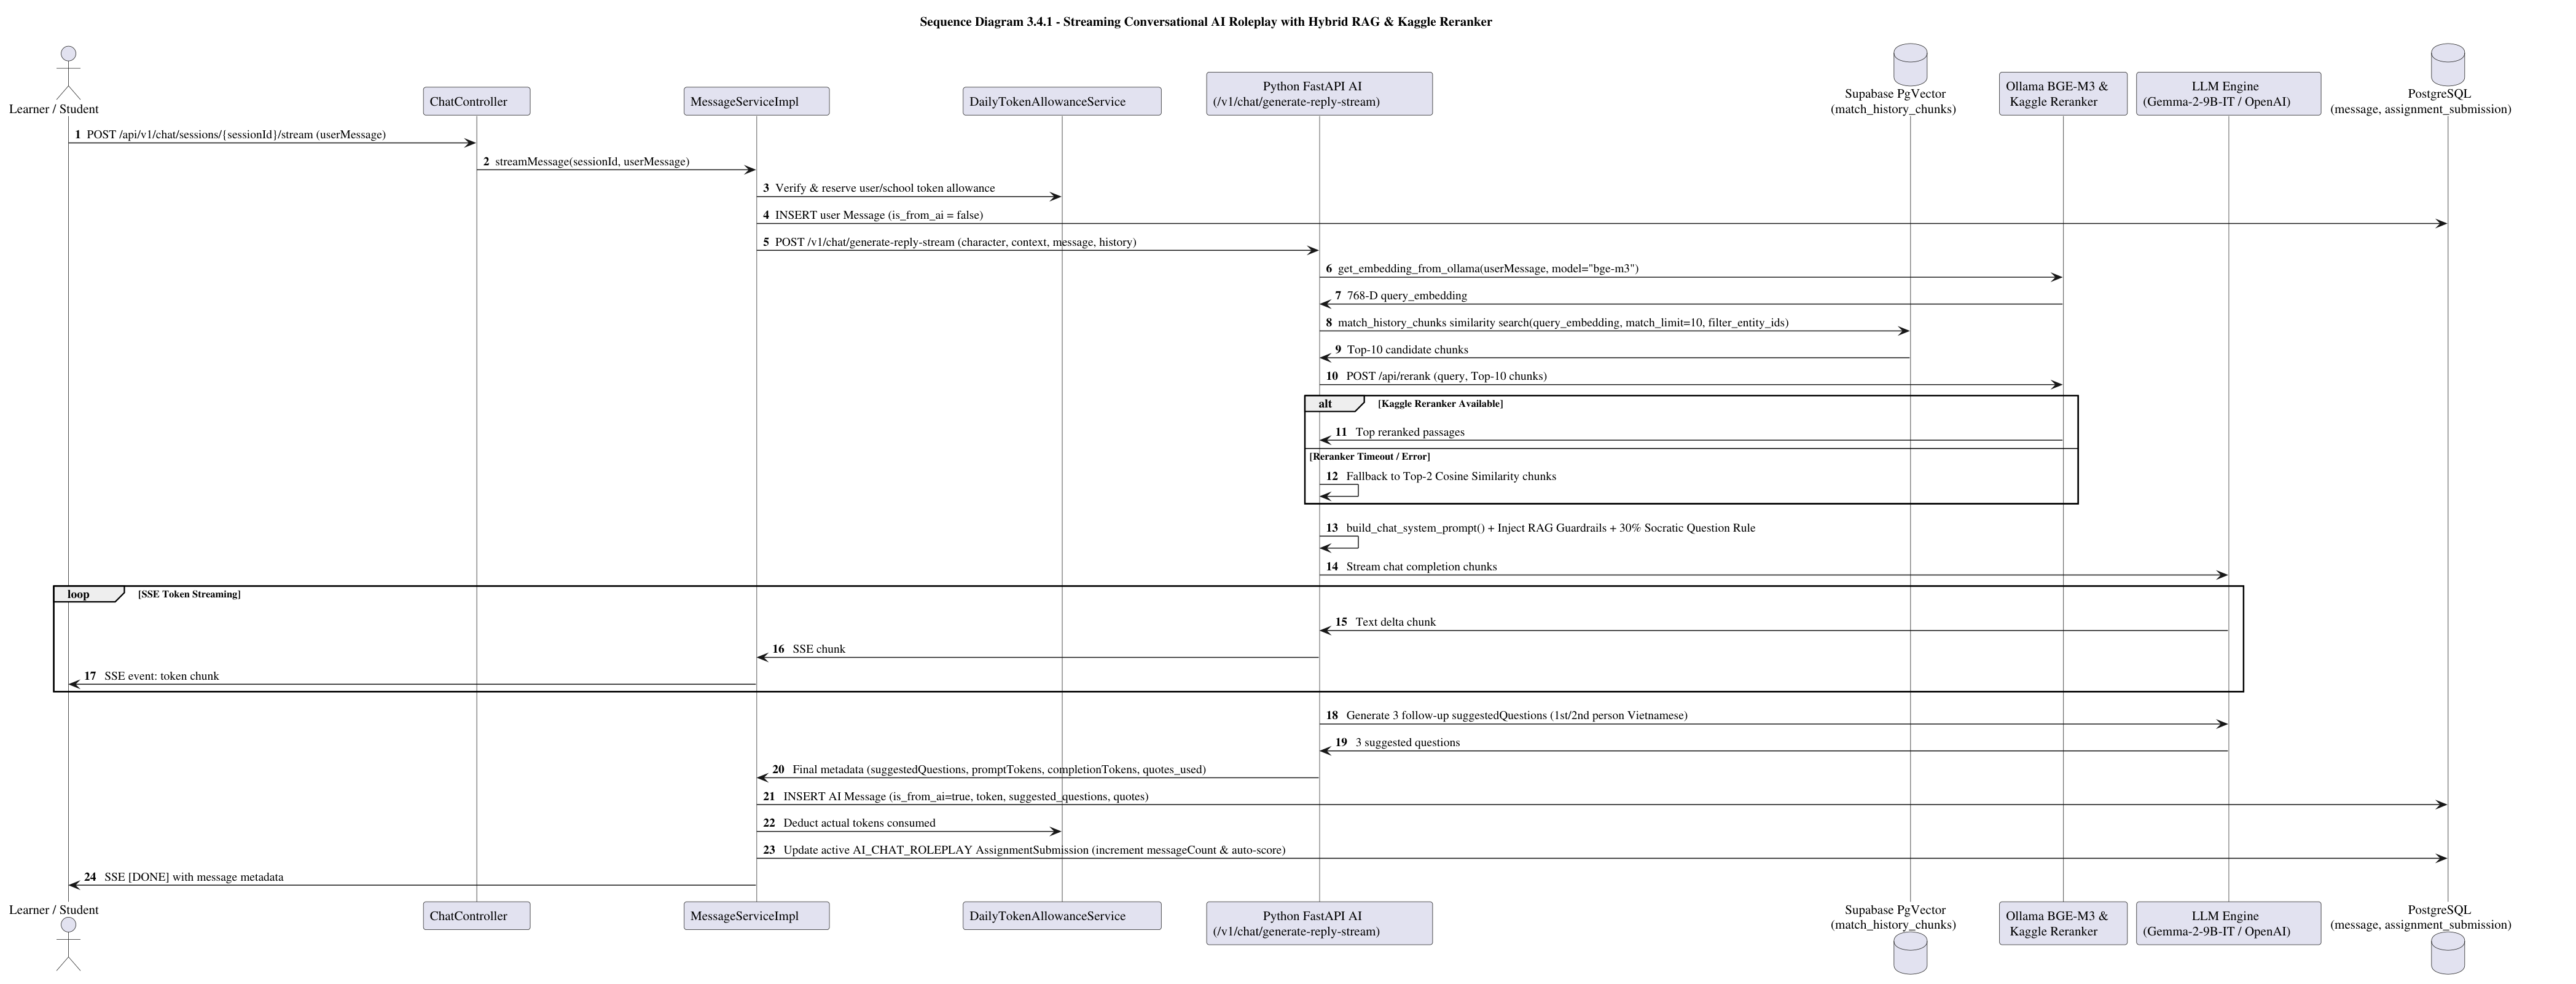
\includegraphics[width=0.98\textwidth]{figures/seq_07_ai_roleplay_chat_rag.png}
    \caption{Sequence Diagram -- Streaming Conversational AI Roleplay with Hybrid RAG \& Kaggle Reranker}
    \label{fig:seq_07_ai_roleplay_chat_rag}
\end{figure}

\newpage
\subsection{Quiz Engine, Question Bank \& Classroom Assignments}

\subsubsection{Class Diagram: Quiz Engine, Question Bank \& Classroom Assignments}

\begin{figure}[H]
    \centering
    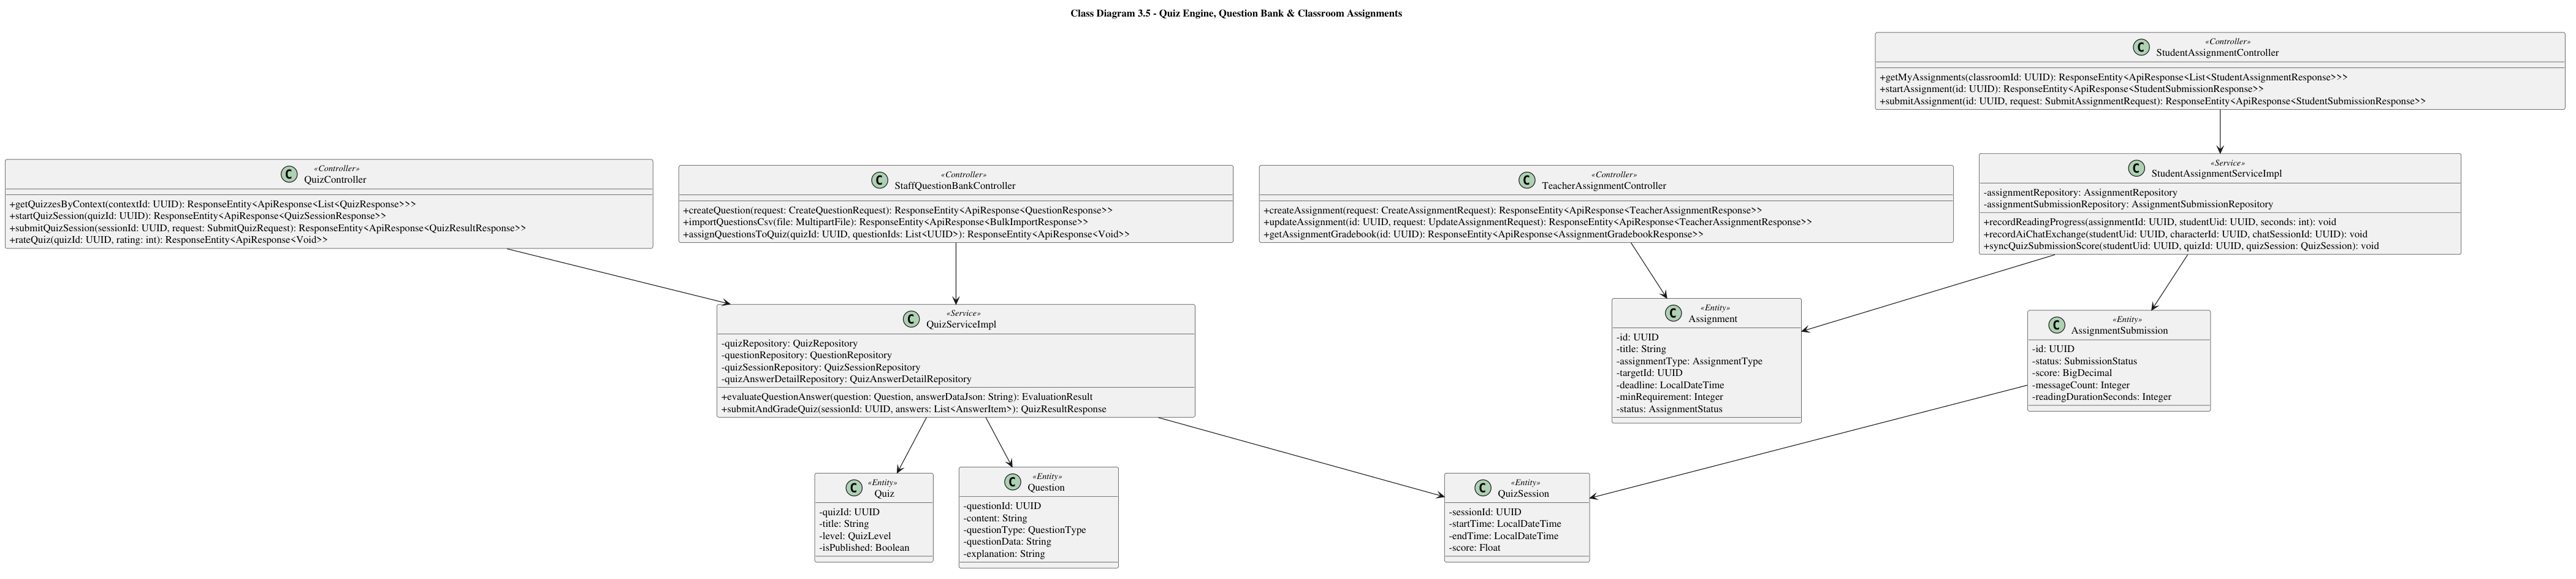
\includegraphics[width=0.98\textwidth]{figures/cls_05_quiz_and_assignment.png}
    \caption{Class Diagram -- Quiz Engine, Question Bank \& Classroom Assignments}
    \label{fig:cls_05_quiz_and_assignment}
\end{figure}

\begin{longtable}{|L{5.5cm}|L{10.0cm}|}
\hline
\rowcolor{tableheader}
\textbf{Class} & \textbf{Description} \\
\hline
\endhead
\texttt{QuizController} / \texttt{StaffQuizController} & REST API controllers managing learner quiz attempts, submissions, ratings, question issue reports, and staff quiz creation/publication. \\
\hline
\texttt{StaffQuestionBankController} & REST API controller (\texttt{/api/v1/staff/question-bank}) supporting polymorphic question creation (\texttt{MULTIPLE\_CHOICE}, \texttt{FILL\_IN\_BLANK}, \texttt{MATCHING}), bulk CSV import, and many-to-many quiz linking. \\
\hline
\texttt{TeacherAssignmentController} & REST API controller (\texttt{/api/v1/teacher/assignments}) enabling teachers to create, update, cancel, or archive classroom assignments and view class gradebooks. \\
\hline
\texttt{StudentAssignmentController} & REST API controller (\texttt{/api/v1/student/assignments}) allowing students to view assigned tasks, start work, log reading duration, and submit completed assignments. \\
\hline
\texttt{QuizServiceImpl} & Evaluates polymorphic JSON question payloads (\texttt{question\_data} vs. \texttt{answer\_data}), computes weighted scores on a 10-point scale, persists \texttt{QuizAnswerDetail} records, and triggers assignment/quest hooks. \\
\hline
\texttt{TeacherAssignmentServiceImpl} / \texttt{StudentAssignmentServiceImpl} & Orchestrates classroom assignment lifecycles, auto-initializes student submission rows, synchronizes AI chat and quiz scores, and classifies on-time (\texttt{SUBMITTED}) vs. late (\texttt{LATE\_SUBMITTED}) completions. \\
\hline
\texttt{Quiz}, \texttt{Question}, \texttt{QuizQuestion}, \texttt{QuizSession}, \texttt{Assignment}, \texttt{AssignmentSubmission} & Domain entities modeling the polymorphic question bank, quiz attempts, classroom assignments, and student gradebook submissions. \\
\hline
\caption{Class Descriptions -- Quiz Engine, Question Bank \& Classroom Assignments}
\label{tab:cls_05_quiz_and_assignment}
\end{longtable}

\subsubsection{Sequence Diagrams: Multi-Type Quiz Grading \& Classroom Assignments}

\begin{figure}[H]
    \centering
    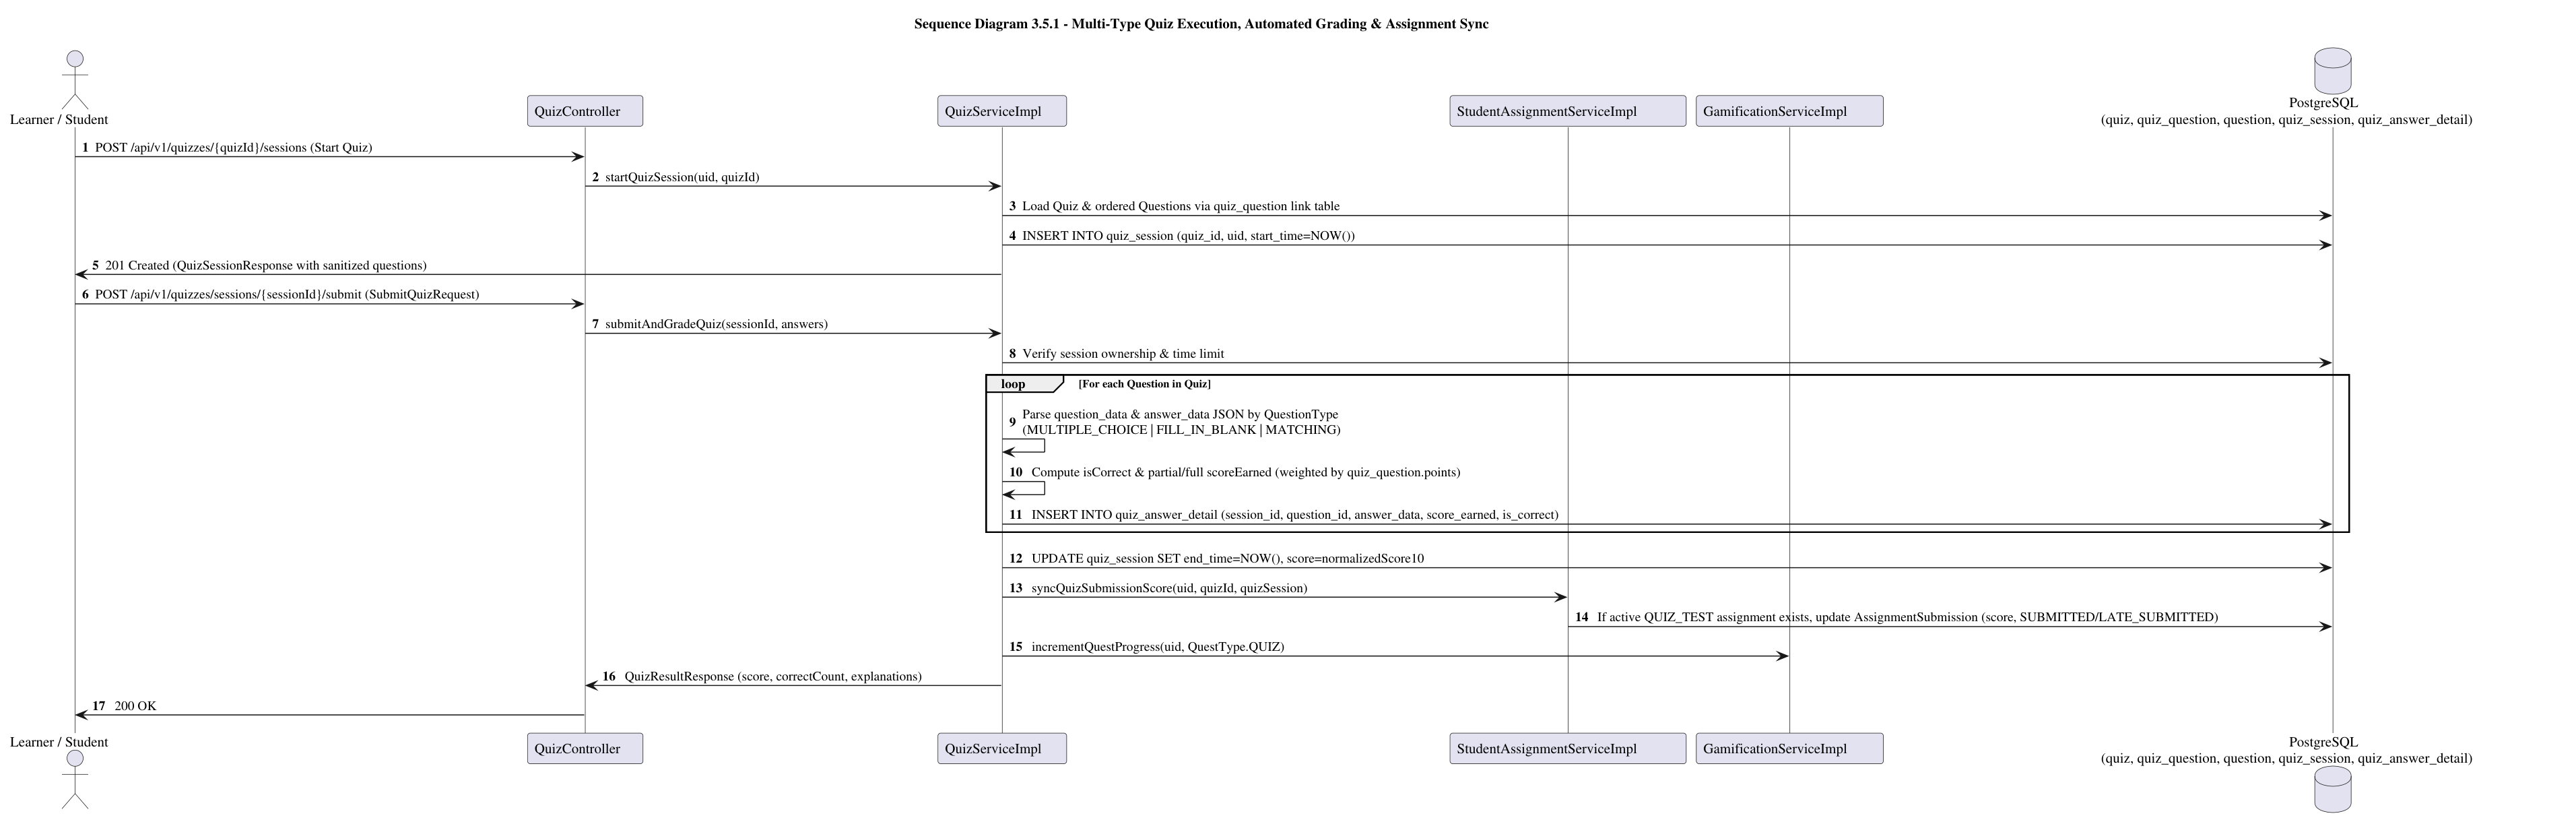
\includegraphics[width=0.98\textwidth]{figures/seq_08_quiz_attempt_and_grading.png}
    \caption{Sequence Diagram -- Multi-Type Quiz Execution, Automated Grading \& Assignment Sync}
    \label{fig:seq_08_quiz_attempt_and_grading}
\end{figure}

\begin{figure}[H]
    \centering
    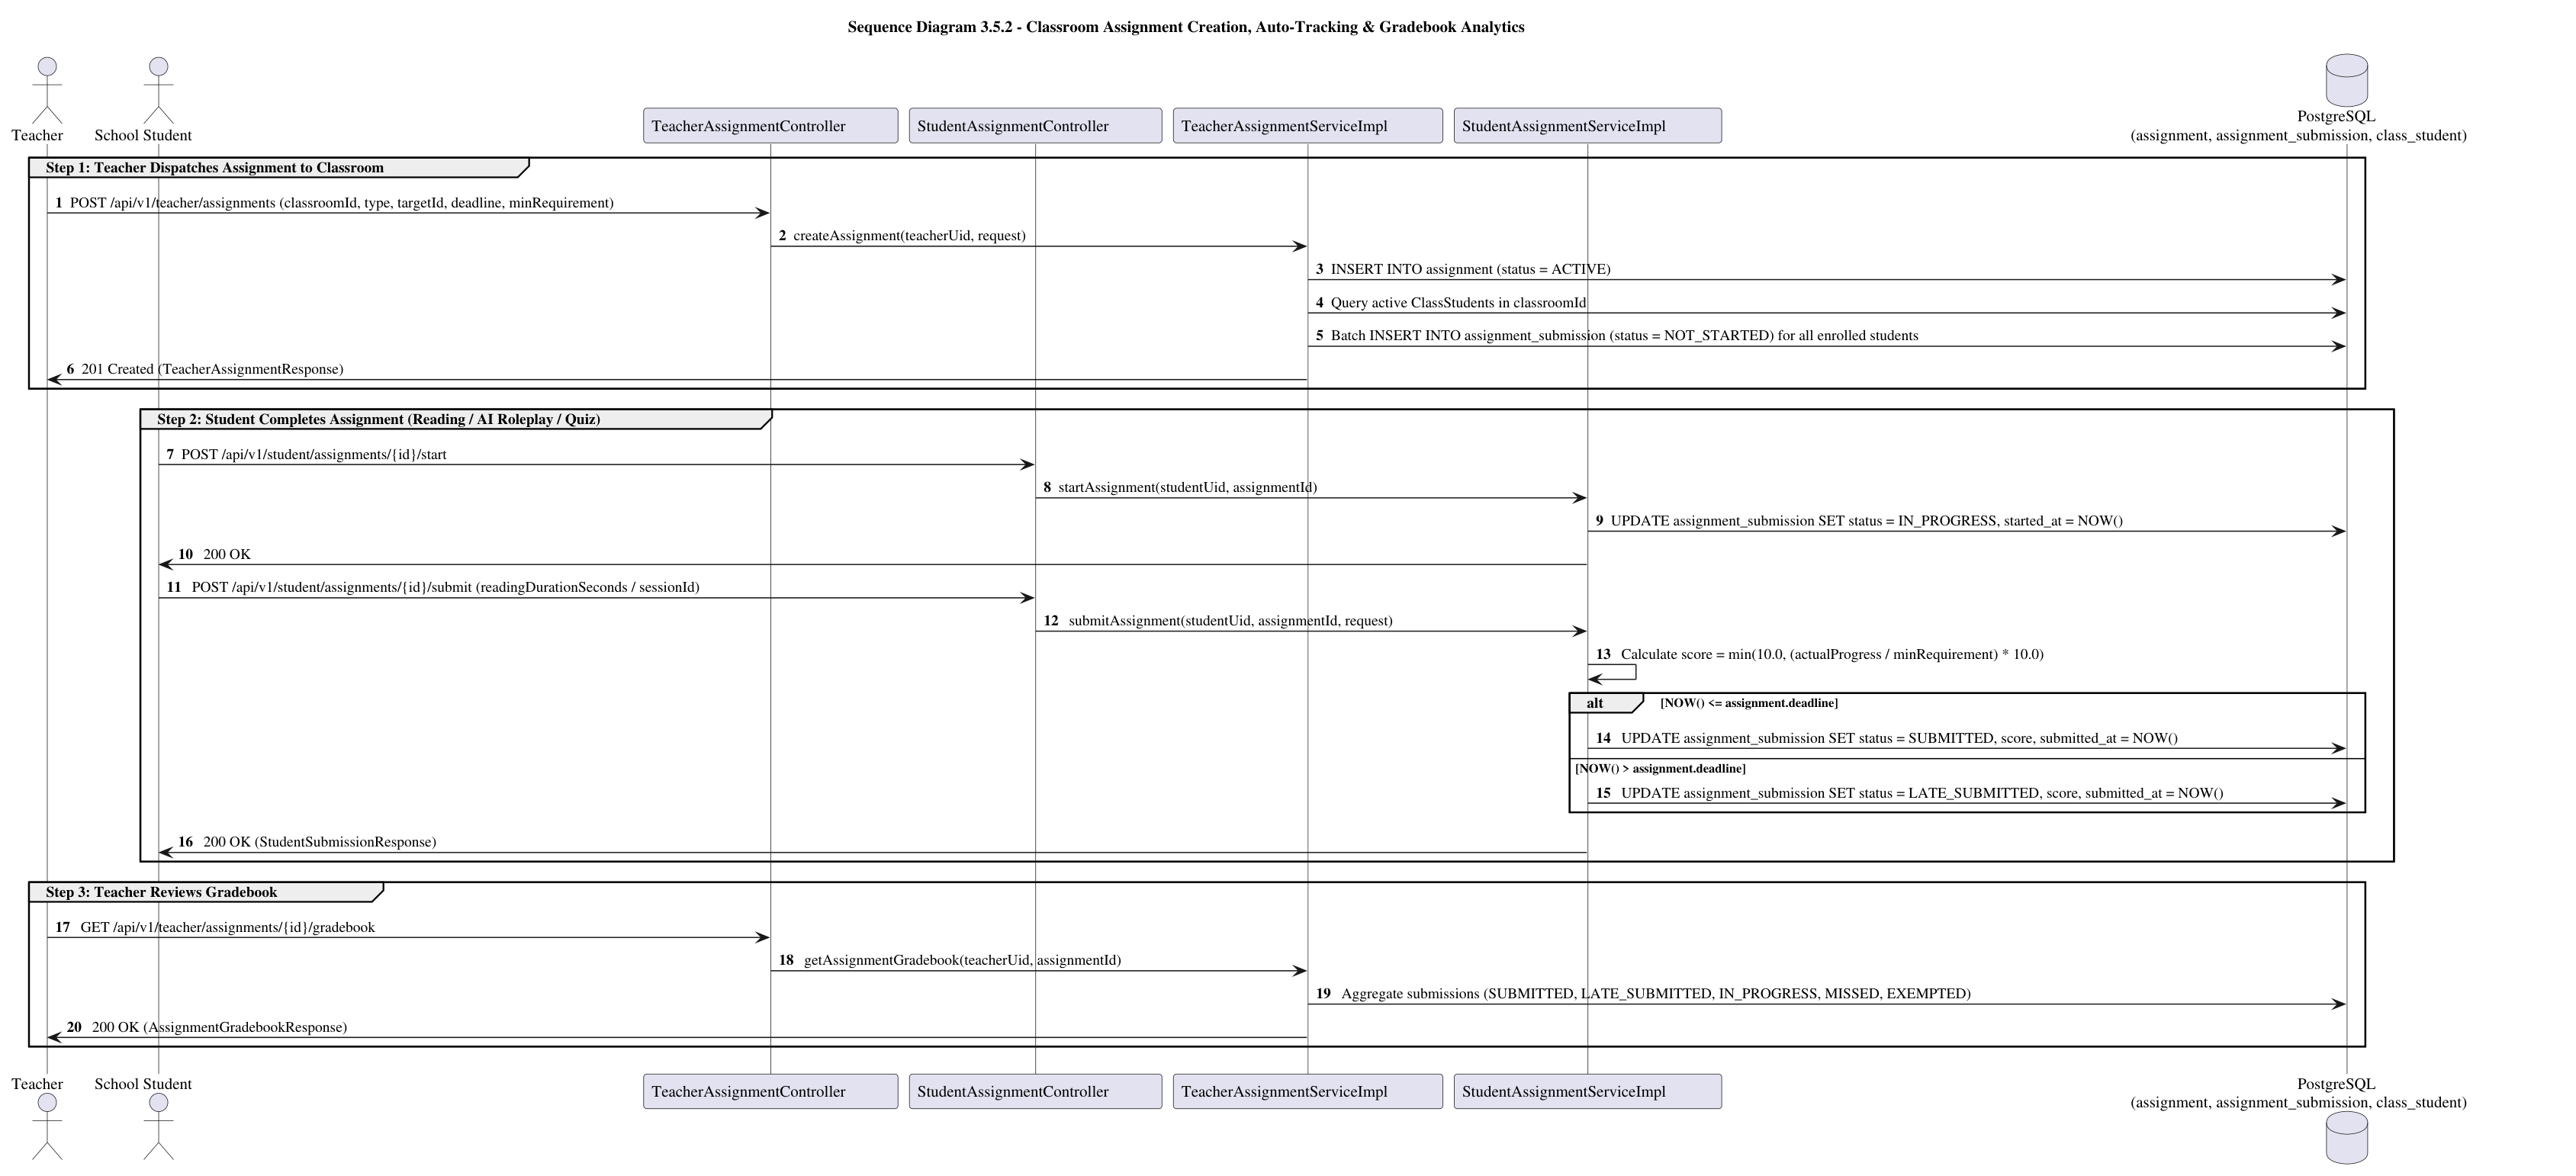
\includegraphics[width=0.98\textwidth]{figures/seq_09_classroom_assignment_submission.png}
    \caption{Sequence Diagram -- Classroom Assignment Creation, Auto-Tracking \& Gradebook Analytics}
    \label{fig:seq_09_classroom_assignment_submission}
\end{figure}

\newpage
\subsection{B2C Subscription, Gamification \& PayOS Payment Fulfillment}

\subsubsection{Class Diagram: B2C Subscription, Gamification \& PayOS Payment Fulfillment}

\begin{figure}[H]
    \centering
    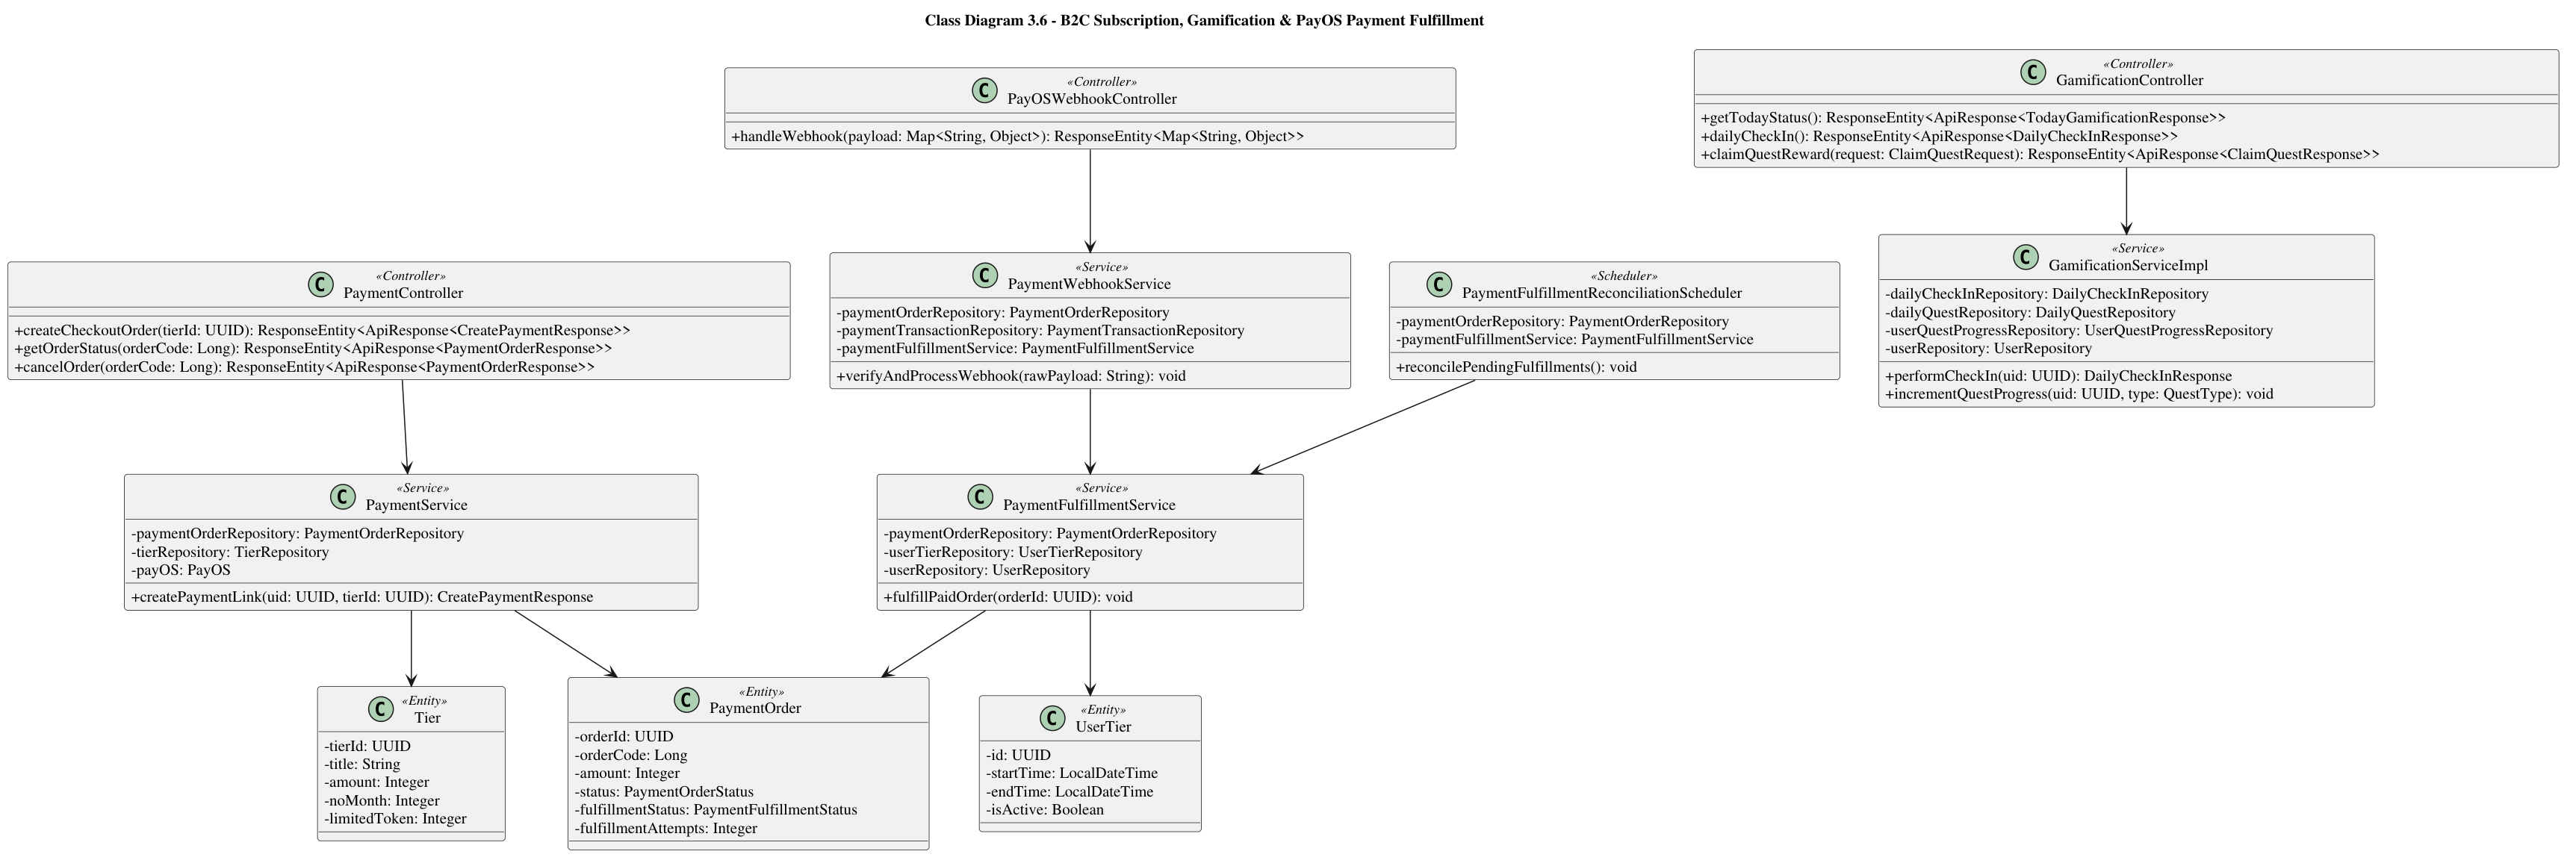
\includegraphics[width=0.98\textwidth]{figures/cls_06_payment_and_gamification.png}
    \caption{Class Diagram -- B2C Subscription, Gamification \& PayOS Payment Fulfillment}
    \label{fig:cls_06_payment_and_gamification}
\end{figure}

\begin{longtable}{|L{5.8cm}|L{9.7cm}|}
\hline
\rowcolor{tableheader}
\textbf{Class} & \textbf{Description} \\
\hline
\endhead
\texttt{PaymentController} & REST API controller (\texttt{/api/v1/payments}) for B2C customers to initiate subscription tier checkouts, poll order status, and cancel pending orders. \\
\hline
\texttt{PayOSWebhookController} & Public webhook endpoint (\texttt{/api/v1/payments/payos/webhook}) receiving asynchronous payment notifications from PayOS. \\
\hline
\texttt{GamificationController} / \texttt{StaffQuestController} & REST API controllers managing daily streak check-ins, daily quest progress queries, token reward claims, and staff quest configurations. \\
\hline
\texttt{PaymentService} / \texttt{PaymentWebhookService} & Generates unique numeric order codes, creates PayOS checkout links, verifies HMAC-SHA256 webhook signatures, and logs immutable \texttt{PaymentTransaction} records. \\
\hline
\texttt{PaymentFulfillmentService} & Executes idempotent, pessimistic-locked order fulfillment (\texttt{PENDING} $\rightarrow$ \texttt{PROCESSING} $\rightarrow$ \texttt{FULFILLED}), activating \texttt{UserTier} and crediting \texttt{Tier.limitedToken} to the user. \\
\hline
\texttt{PaymentFulfillmentReconciliationScheduler} / \texttt{PaymentExpiryScheduler} & Background Spring \texttt{@Scheduled} jobs that retry unfulfilled \texttt{PAID} orders (up to 5 attempts) and transition stale \texttt{PENDING} orders to \texttt{EXPIRED}. \\
\hline
\texttt{GamificationServiceImpl} & Tracks consecutive daily login streaks (\texttt{DailyCheckIn}) and quest progress (\texttt{UserQuestProgress}) across \texttt{CHAT}, \texttt{QUIZ}, and \texttt{READ\_CONTEXT} activities. \\
\hline
\caption{Class Descriptions -- B2C Subscription, Gamification \& PayOS Payment Fulfillment}
\label{tab:cls_06_payment_and_gamification}
\end{longtable}

\subsubsection{Sequence Diagram: PayOS Checkout \& Resilient Tier Fulfillment}

\begin{figure}[H]
    \centering
    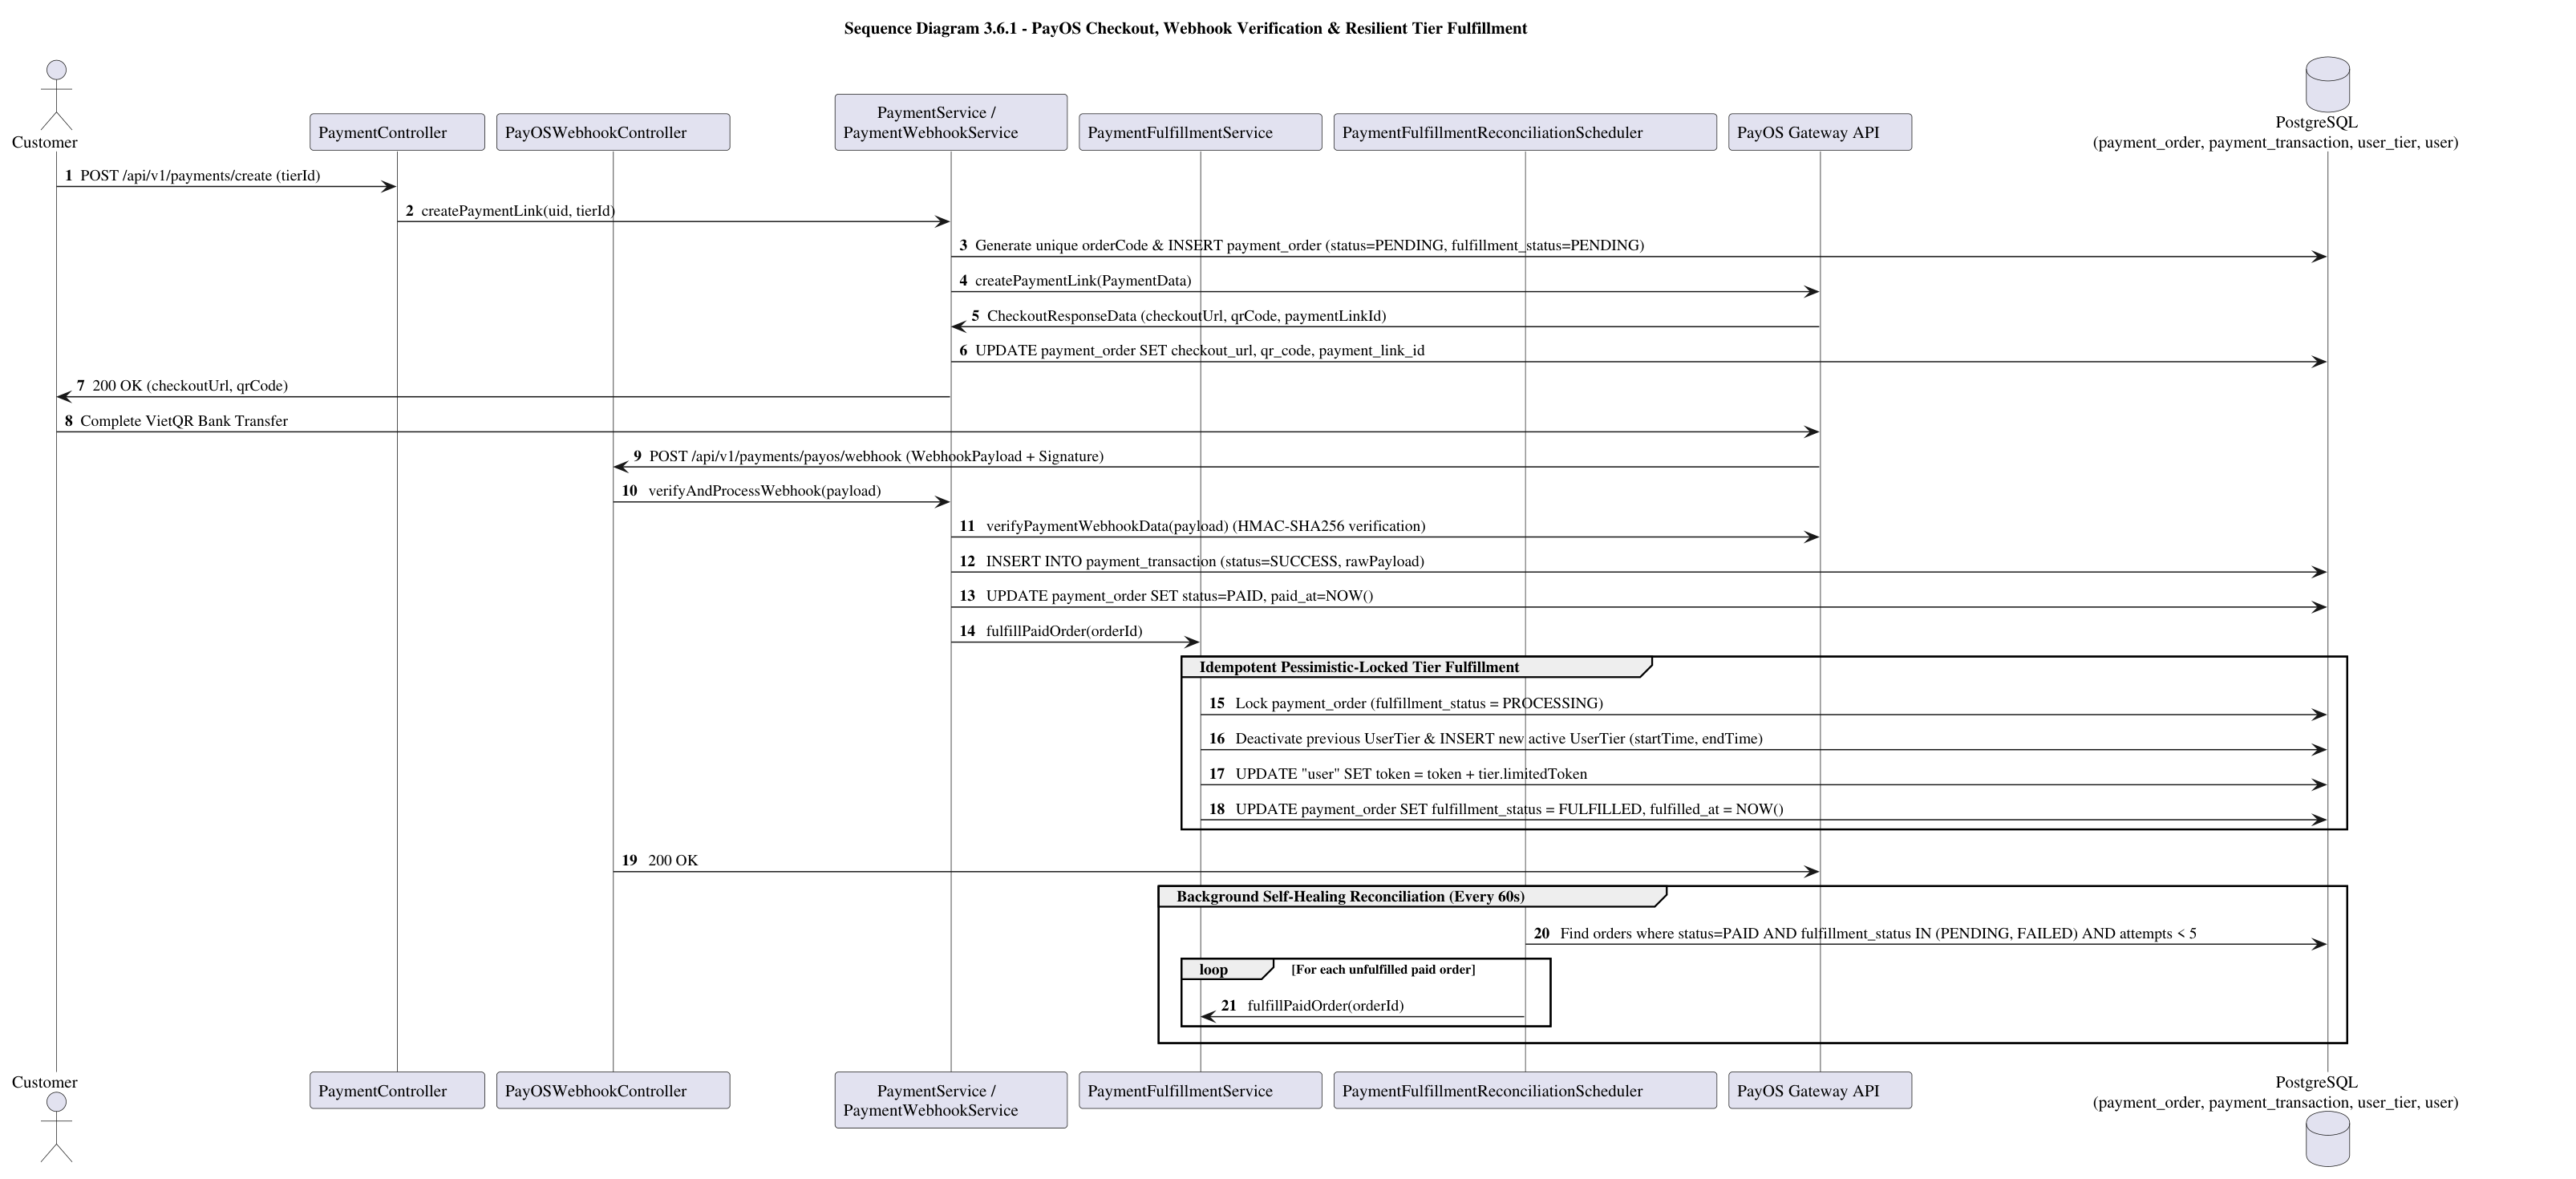
\includegraphics[width=0.98\textwidth]{figures/seq_10_payos_checkout_and_fulfillment.png}
    \caption{Sequence Diagram -- PayOS Checkout, Webhook Verification \& Resilient Tier Fulfillment}
    \label{fig:seq_10_payos_checkout_and_fulfillment}
\end{figure}

\newpage
% ============================================================================
% SECTION 4: ENTITY STATE MACHINES & MAIN WORKFLOW ACTIVITY DIAGRAMS
% ============================================================================
\section{Entity State Machine Diagrams and Main Business Workflows}

\subsection{Entity State Machine Diagrams}

To ensure consistency between the Software Design Document and the domain enumerations (com.historytalk.\ab entity.enums), Figures~\ref{fig:stm_01_content_and_account}, \ref{fig:stm_02_assignment_and_token}, and \ref{fig:stm_03_payment_lifecycle} model the finite state machines of the stateful domain lifecycles in HistoryTalk.

\begin{figure}[htbp]
    \centering
    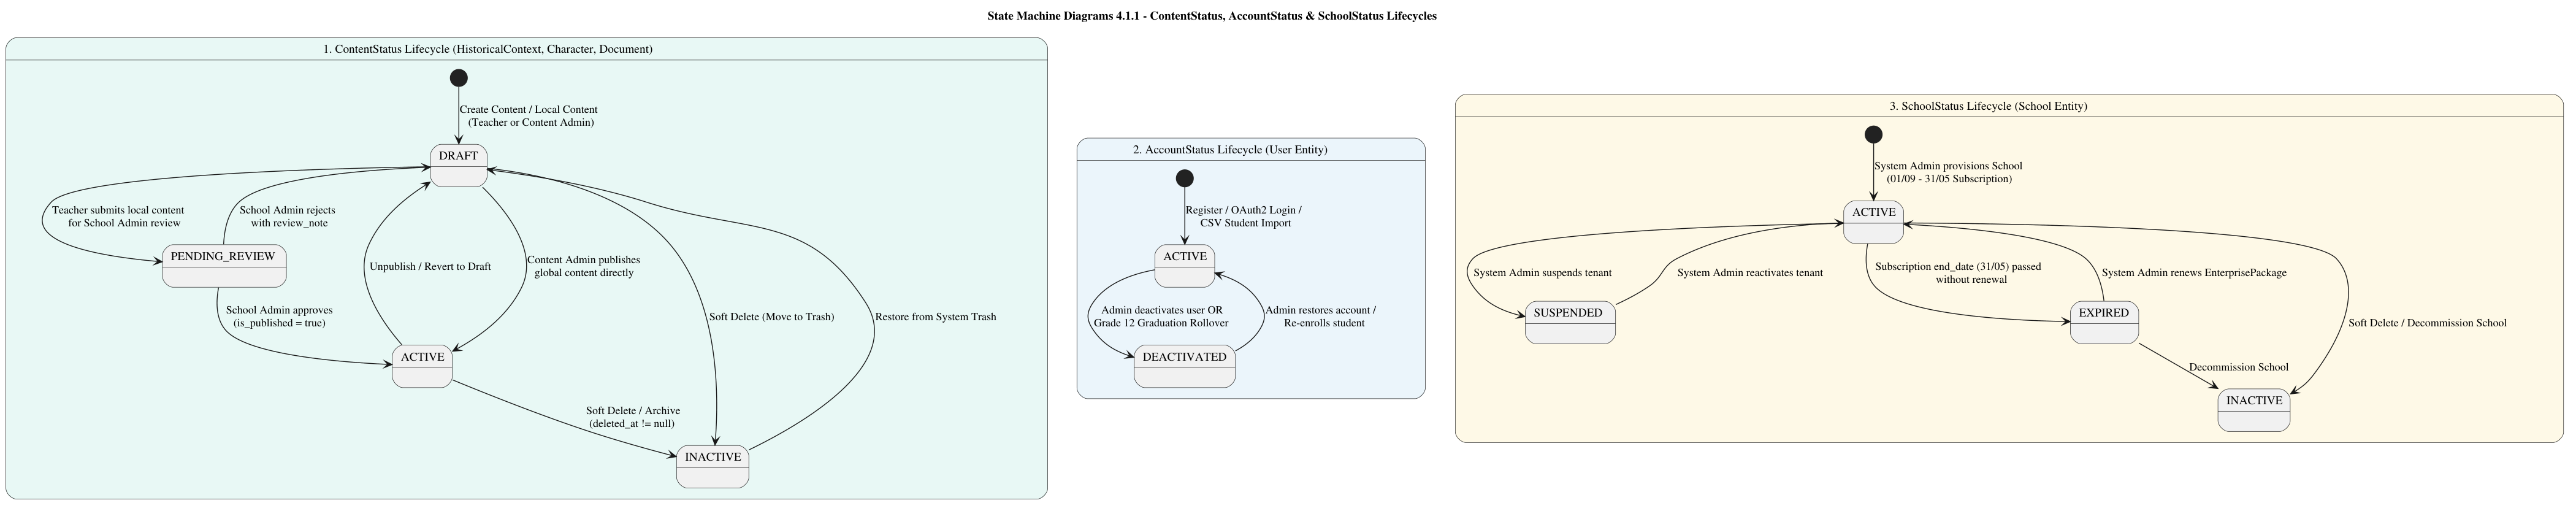
\includegraphics[width=0.98\textwidth,height=0.25\textheight,keepaspectratio]{figures/stm_01_content_and_account.png}
    \caption{State Machine Diagrams -- ContentStatus, AccountStatus and SchoolStatus Lifecycles}
    \label{fig:stm_01_content_and_account}
\end{figure}

\begin{figure}[htbp]
    \centering
    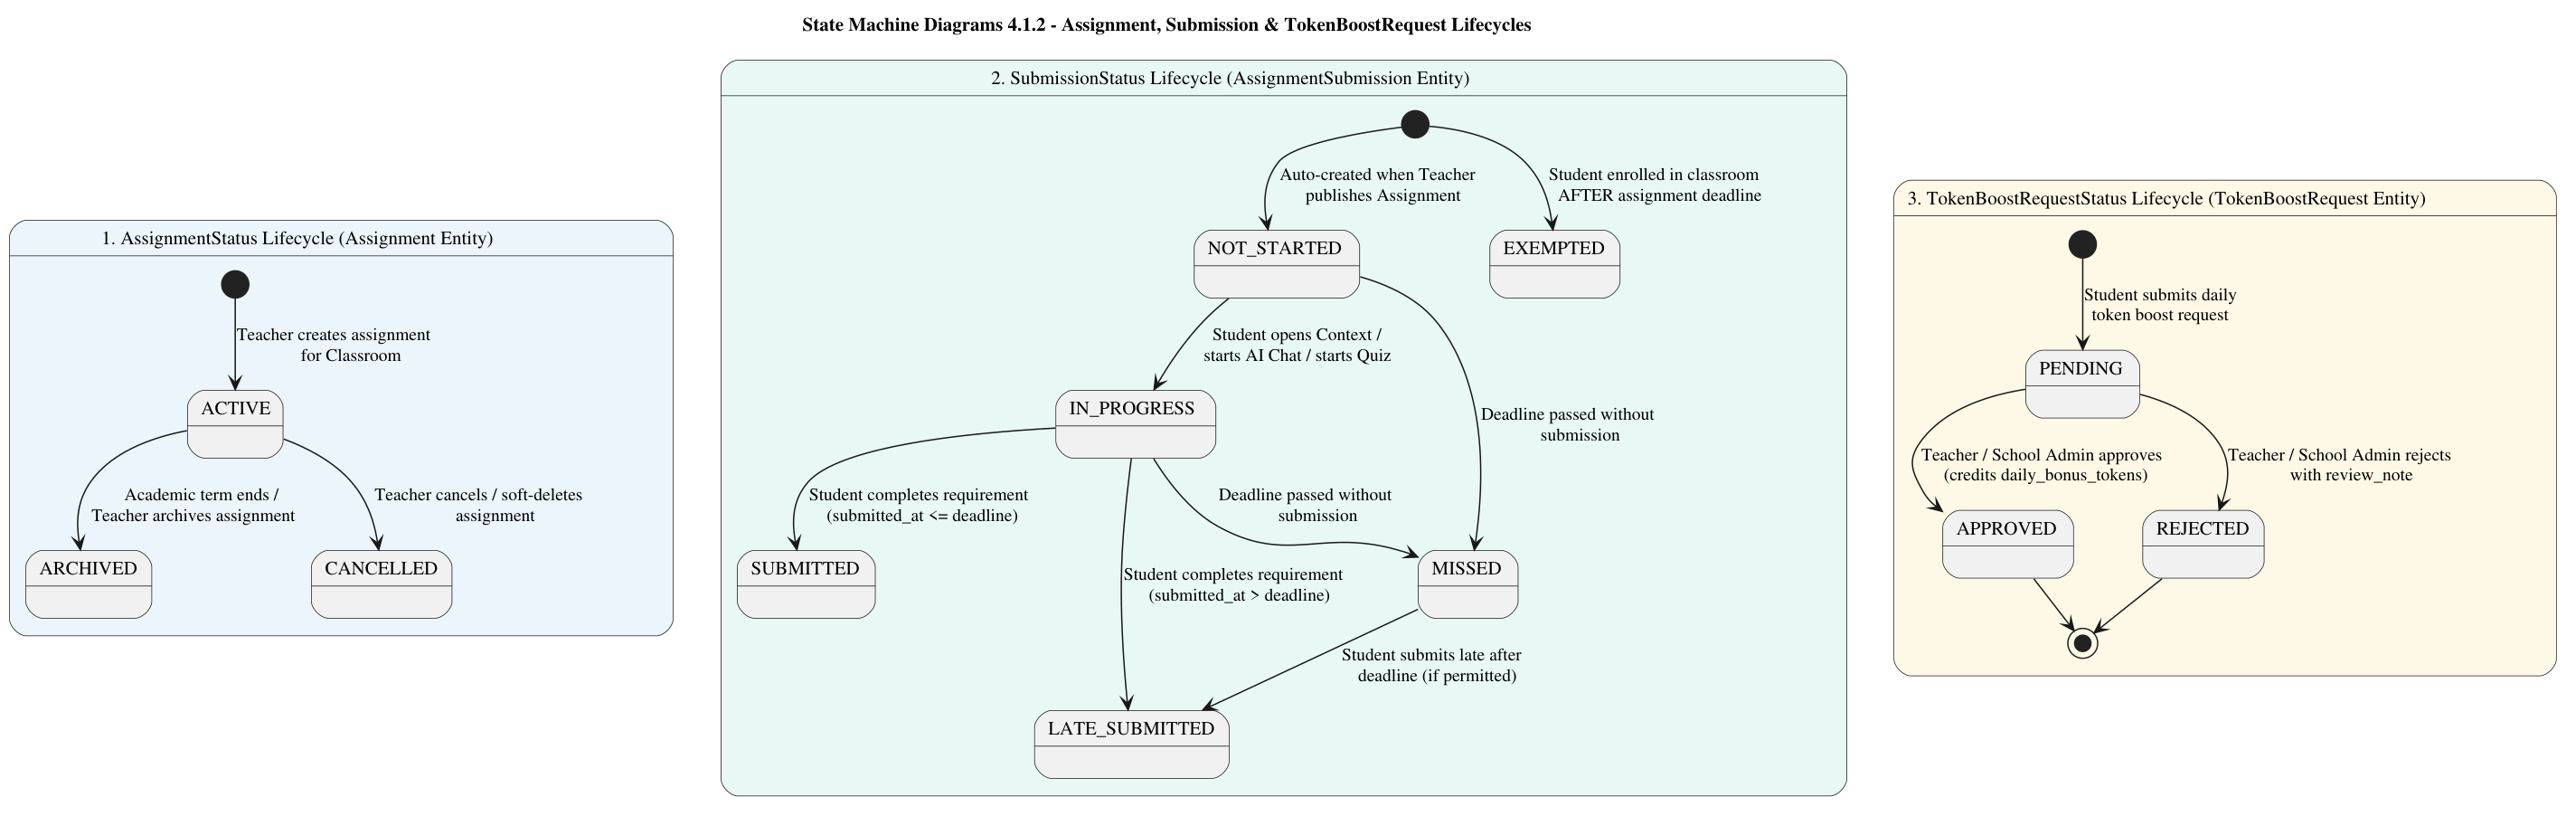
\includegraphics[width=0.98\textwidth,height=0.25\textheight,keepaspectratio]{figures/stm_02_assignment_and_token.png}
    \caption{State Machine Diagrams -- AssignmentStatus, SubmissionStatus and TokenBoostRequestStatus Lifecycles}
    \label{fig:stm_02_assignment_and_token}
\end{figure}

\begin{figure}[htbp]
    \centering
    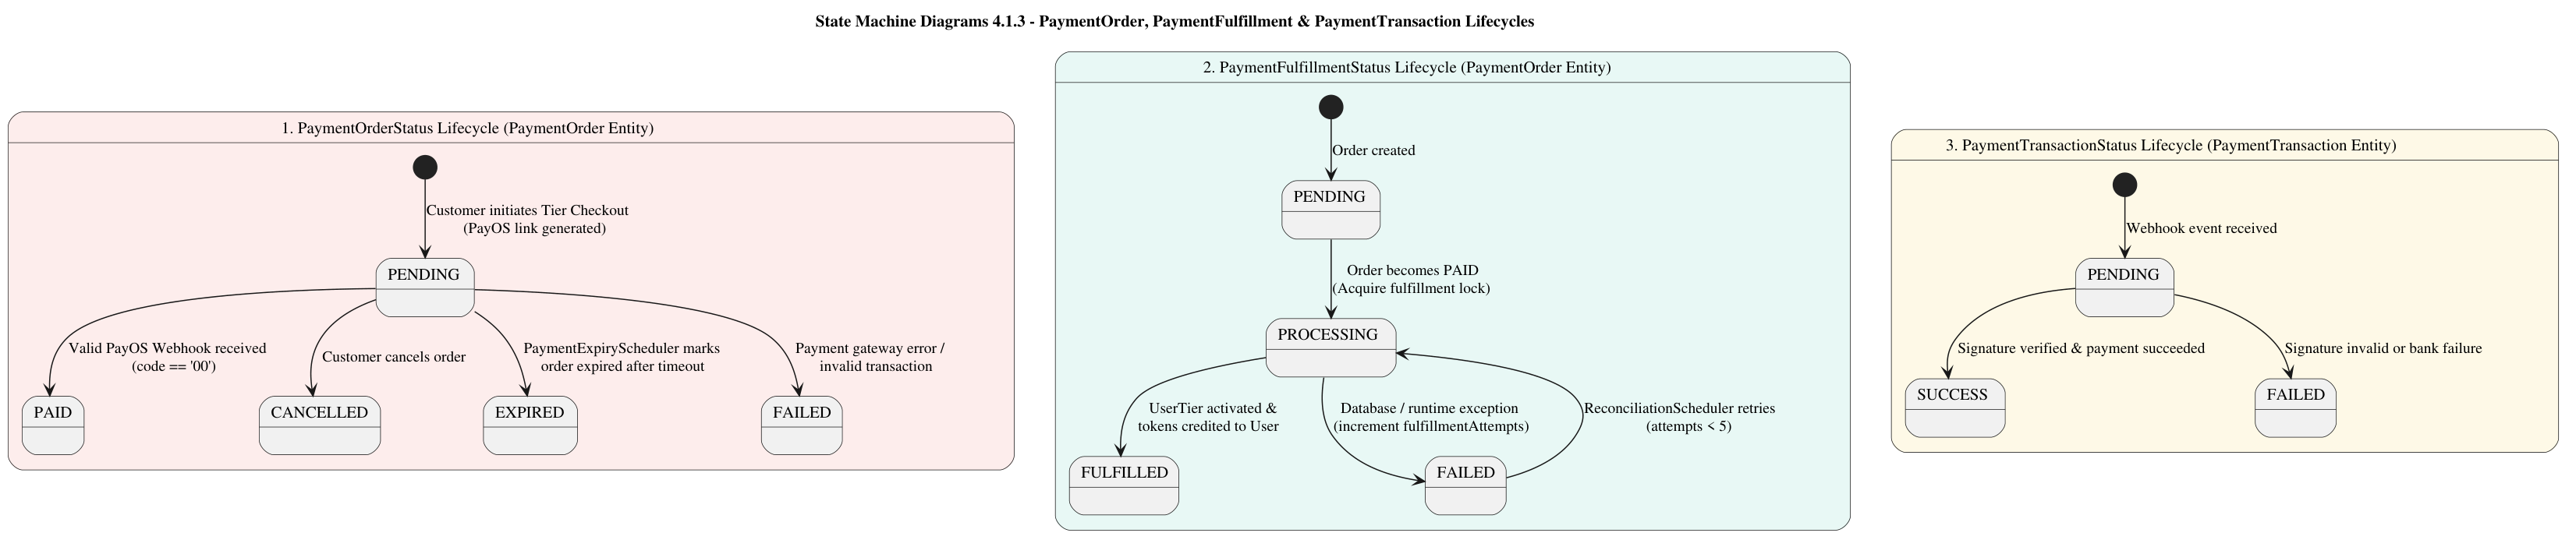
\includegraphics[width=0.98\textwidth,height=0.25\textheight,keepaspectratio]{figures/stm_03_payment_lifecycle.png}
    \caption{State Machine Diagrams -- PaymentOrderStatus, PaymentFulfillmentStatus and PaymentTransactionStatus Lifecycles}
    \label{fig:stm_03_payment_lifecycle}
\end{figure}

\paragraph{State Transition and Trigger Traceability Matrix}
Table~\ref{tab:state_transitions} maps each state enumeration in the system to its valid transitions and triggering API endpoints or schedulers.

\footnotesize
\begin{longtable}{|L{3.3cm}|L{2.6cm}|L{3.5cm}|L{4.7cm}|}
\hline
\rowcolor{tableheader}
\textbf{Entity / Enum} & \textbf{States} & \textbf{Valid Transitions} & \textbf{Triggering Feature / API / Scheduler} \\
\hline
\endhead
HistoricalContext, Character, Document\newline(ContentStatus) & DRAFT, PENDING\_\ab REVIEW, ACTIVE, INACTIVE & DRAFT $\rightarrow$ PENDING\_\ab REVIEW\newline PENDING\_\ab REVIEW $\rightarrow$ ACTIVE / DRAFT\newline DRAFT $\leftrightarrow$ ACTIVE\newline DRAFT/ACTIVE $\rightarrow$ INACTIVE\newline INACTIVE $\rightarrow$ DRAFT & Teacher submits local content (PUT /submit-review); School Admin approves or rejects (PUT /local-content/\ab \{id\}/status); Content Admin publishes, deletes, or restores (SystemTrash\ab Controller). \\
\hline
User\newline(AccountStatus) & ACTIVE, DEACTIVATED & ACTIVE $\leftrightarrow$ DEACTIVATED & Admin deactivates or restores user (AdminUser\ab Controller); End-of-year Grade 12 rollover (AcademicLifecycle\ab ServiceImpl). \\
\hline
School\newline(SchoolStatus) & ACTIVE, INACTIVE, SUSPENDED, EXPIRED & ACTIVE $\leftrightarrow$ SUSPENDED\newline ACTIVE $\leftrightarrow$ EXPIRED\newline ACTIVE/EXPIRED $\rightarrow$ INACTIVE & System Admin updates status or renews package (AdminSchool\ab Controller); Subscription expiry check after 31/05. \\
\hline
Assignment\newline(AssignmentStatus) & ACTIVE, CANCELLED, ARCHIVED & ACTIVE $\rightarrow$ ARCHIVED\newline ACTIVE $\rightarrow$ CANCELLED & Teacher creates, cancels, or archives classroom assignment (TeacherAssignment\ab Controller). \\
\hline
Assignment\ab Submission\newline(SubmissionStatus) & NOT\_STARTED, IN\_PROGRESS, SUBMITTED, LATE\_\ab SUBMITTED, MISSED, EXEMPTED & NOT\_STARTED $\rightarrow$ IN\_PROGRESS\newline IN\_PROGRESS $\rightarrow$ SUBMITTED / LATE\_\ab SUBMITTED\newline NOT\_STARTED/IN\_PROGRESS $\rightarrow$ MISSED\newline [*] $\rightarrow$ EXEMPTED & Student starts or submits assignment (StudentAssignment\ab Controller); Quiz and Chat sync hooks; Late student enrollment auto-exemption (ClassroomImport\ab Processor). \\
\hline
TokenBoostRequest\newline(TokenBoost\ab RequestStatus) & PENDING, APPROVED, REJECTED & PENDING $\rightarrow$ APPROVED\newline PENDING $\rightarrow$ REJECTED & Student requests boost (POST /token-boost-\ab requests); Teacher or School Admin reviews (PUT /token-boost-\ab requests/\ab \{id\}/review). \\
\hline
PaymentOrder\newline(PaymentOrder\ab Status) & PENDING, PAID, CANCELLED, EXPIRED, FAILED & PENDING $\rightarrow$ PAID / CANCELLED / EXPIRED / FAILED & PayOS Webhook (PayOSWebhook\ab Controller), User cancel (PaymentController), Expiry job (PaymentExpiry\ab Scheduler). \\
\hline
PaymentOrder\newline(PaymentFulfillment\ab Status) & PENDING, PROCESSING, FULFILLED, FAILED & PENDING $\rightarrow$ PROCESSING $\rightarrow$ FULFILLED / FAILED\newline FAILED $\rightarrow$ PROCESSING & PaymentFulfillment\ab Service and PaymentFulfillment\ab Reconciliation\ab Scheduler. \\
\hline
PaymentTransaction\newline(PaymentTransaction\ab Status) & PENDING, SUCCESS, FAILED & PENDING $\rightarrow$ SUCCESS / FAILED & Webhook verification in PaymentWebhook\ab Service. \\
\hline
\caption{Complete State Machine Traceability Matrix}
\label{tab:state_transitions}
\end{longtable}
\normalsize

\newpage
\subsection{Main Business Workflow Activity Diagrams}

HistoryTalk defines five end-to-end Main Business Workflows (WF-01 to WF-05), each owned by one team member in alignment with the Project Management Plan (Report 2 RACI Matrix), involving multiple actors and transitioning the state of core domain entities.

{\small
\begin{longtable}{|C{1.1cm}|L{3.2cm}|L{2.3cm}|L{2.5cm}|L{4.8cm}|}
\hline
\rowcolor{tableheader}
\textbf{ID} & \textbf{Workflow Name} & \textbf{Owner} & \textbf{Actors Involved} & \textbf{Primary Entities \& State Changes} \\
\hline
\endhead
WF-01 & B2B School Onboarding, Classroom Management \& Student Analytics & \vn{Trần Quốc Dinh}\newline(SE196495) & System Admin, School Admin, Teacher, School Student & School (ACTIVE), Classroom (ACTIVE), User (ACTIVE), ClassStudent, Assignment\ab Submission (EXEMPTED) \\
\hline
WF-02 & Global Content Management, PDF/OCR Document Ingestion \& Multi-Tenant Access & \vn{Võ Đồng Đức Khải}\newline(SE196405) & Content Admin, Teacher, School Admin & Historical\ab Context, Character, Document (DRAFT $\rightarrow$ PENDING\_\ab REVIEW $\rightarrow$ ACTIVE), VectorChunk \\
\hline
WF-03 & Grounded AI Historical Roleplay Chat, RAG Retrieval \& Token Quota Management & \vn{Nguyễn Minh Trí}\newline(SE192645) & School Student / Customer, Teacher, School Admin & ChatSession, Message, User (dailyTokens\ab Used), TokenBoost\ab Request (PENDING $\rightarrow$ APPROVED) \\
\hline
WF-04 & Timed Quiz Assessment Engine, Interactive Map \& PayOS Payment Fulfillment & \vn{Đỗ Quốc Bảo}\newline(SE193803) & Teacher, School Student, Customer, PayOS Gateway & Assignment (ACTIVE), QuizSession, QuizAnswer\ab Detail, PaymentOrder (PENDING $\rightarrow$ PAID, FULFILLED) \\
\hline
WF-05 & Frontend Client Interactive Learning Workflows, Classroom Submissions \& Daily Quests & \vn{Nguyễn Công Thành}\newline(SE196309) & School Student, Customer, Teacher & Assignment\ab Submission (NOT\_STARTED $\rightarrow$ IN\_PROGRESS $\rightarrow$ SUBMITTED), UserQuest\ab Progress (claimed), DailyCheckIn \\
\hline
\caption{Main Business Workflows Summary and Ownership Matrix}
\label{tab:main_workflows}
\end{longtable}
}

\begin{figure}[htbp]
    \centering
    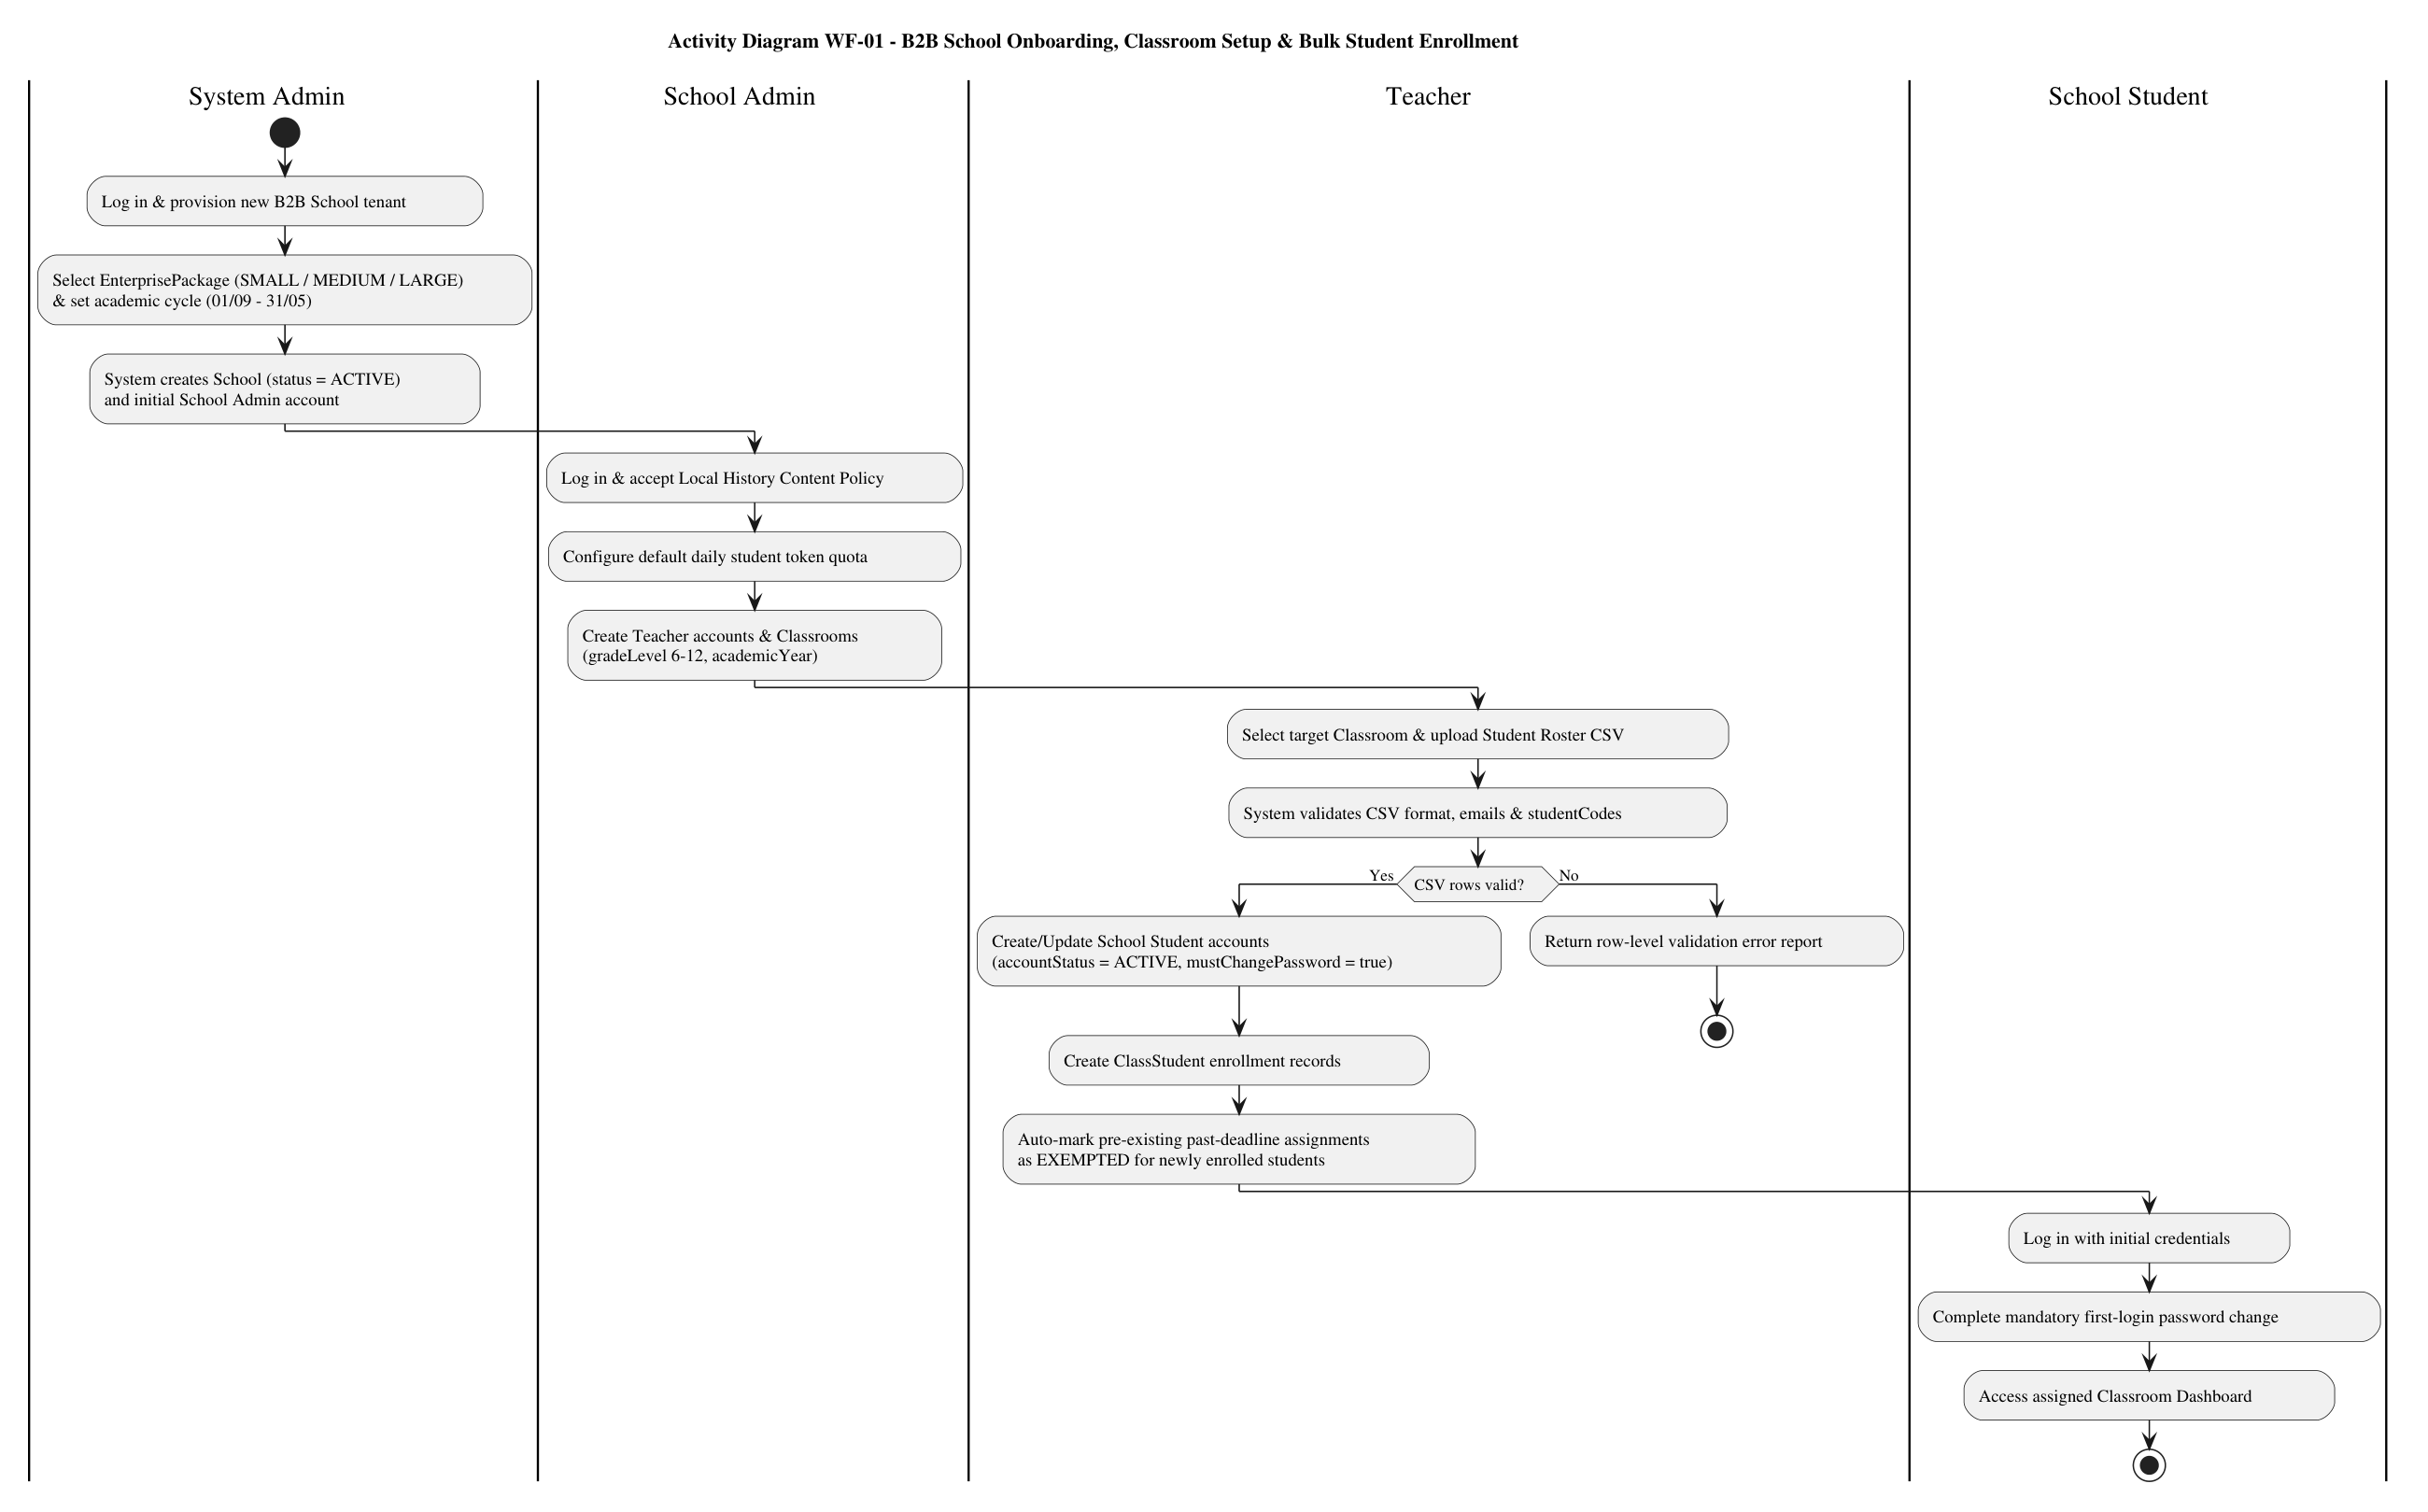
\includegraphics[width=0.95\textwidth,height=0.42\textheight,keepaspectratio]{figures/act_wf01_school_onboarding_and_enrollment.png}
    \caption{Activity Diagram WF-01 -- B2B School Onboarding, Classroom Setup and Bulk Student Enrollment}
    \label{fig:act_wf01}
\end{figure}

\begin{figure}[htbp]
    \centering
    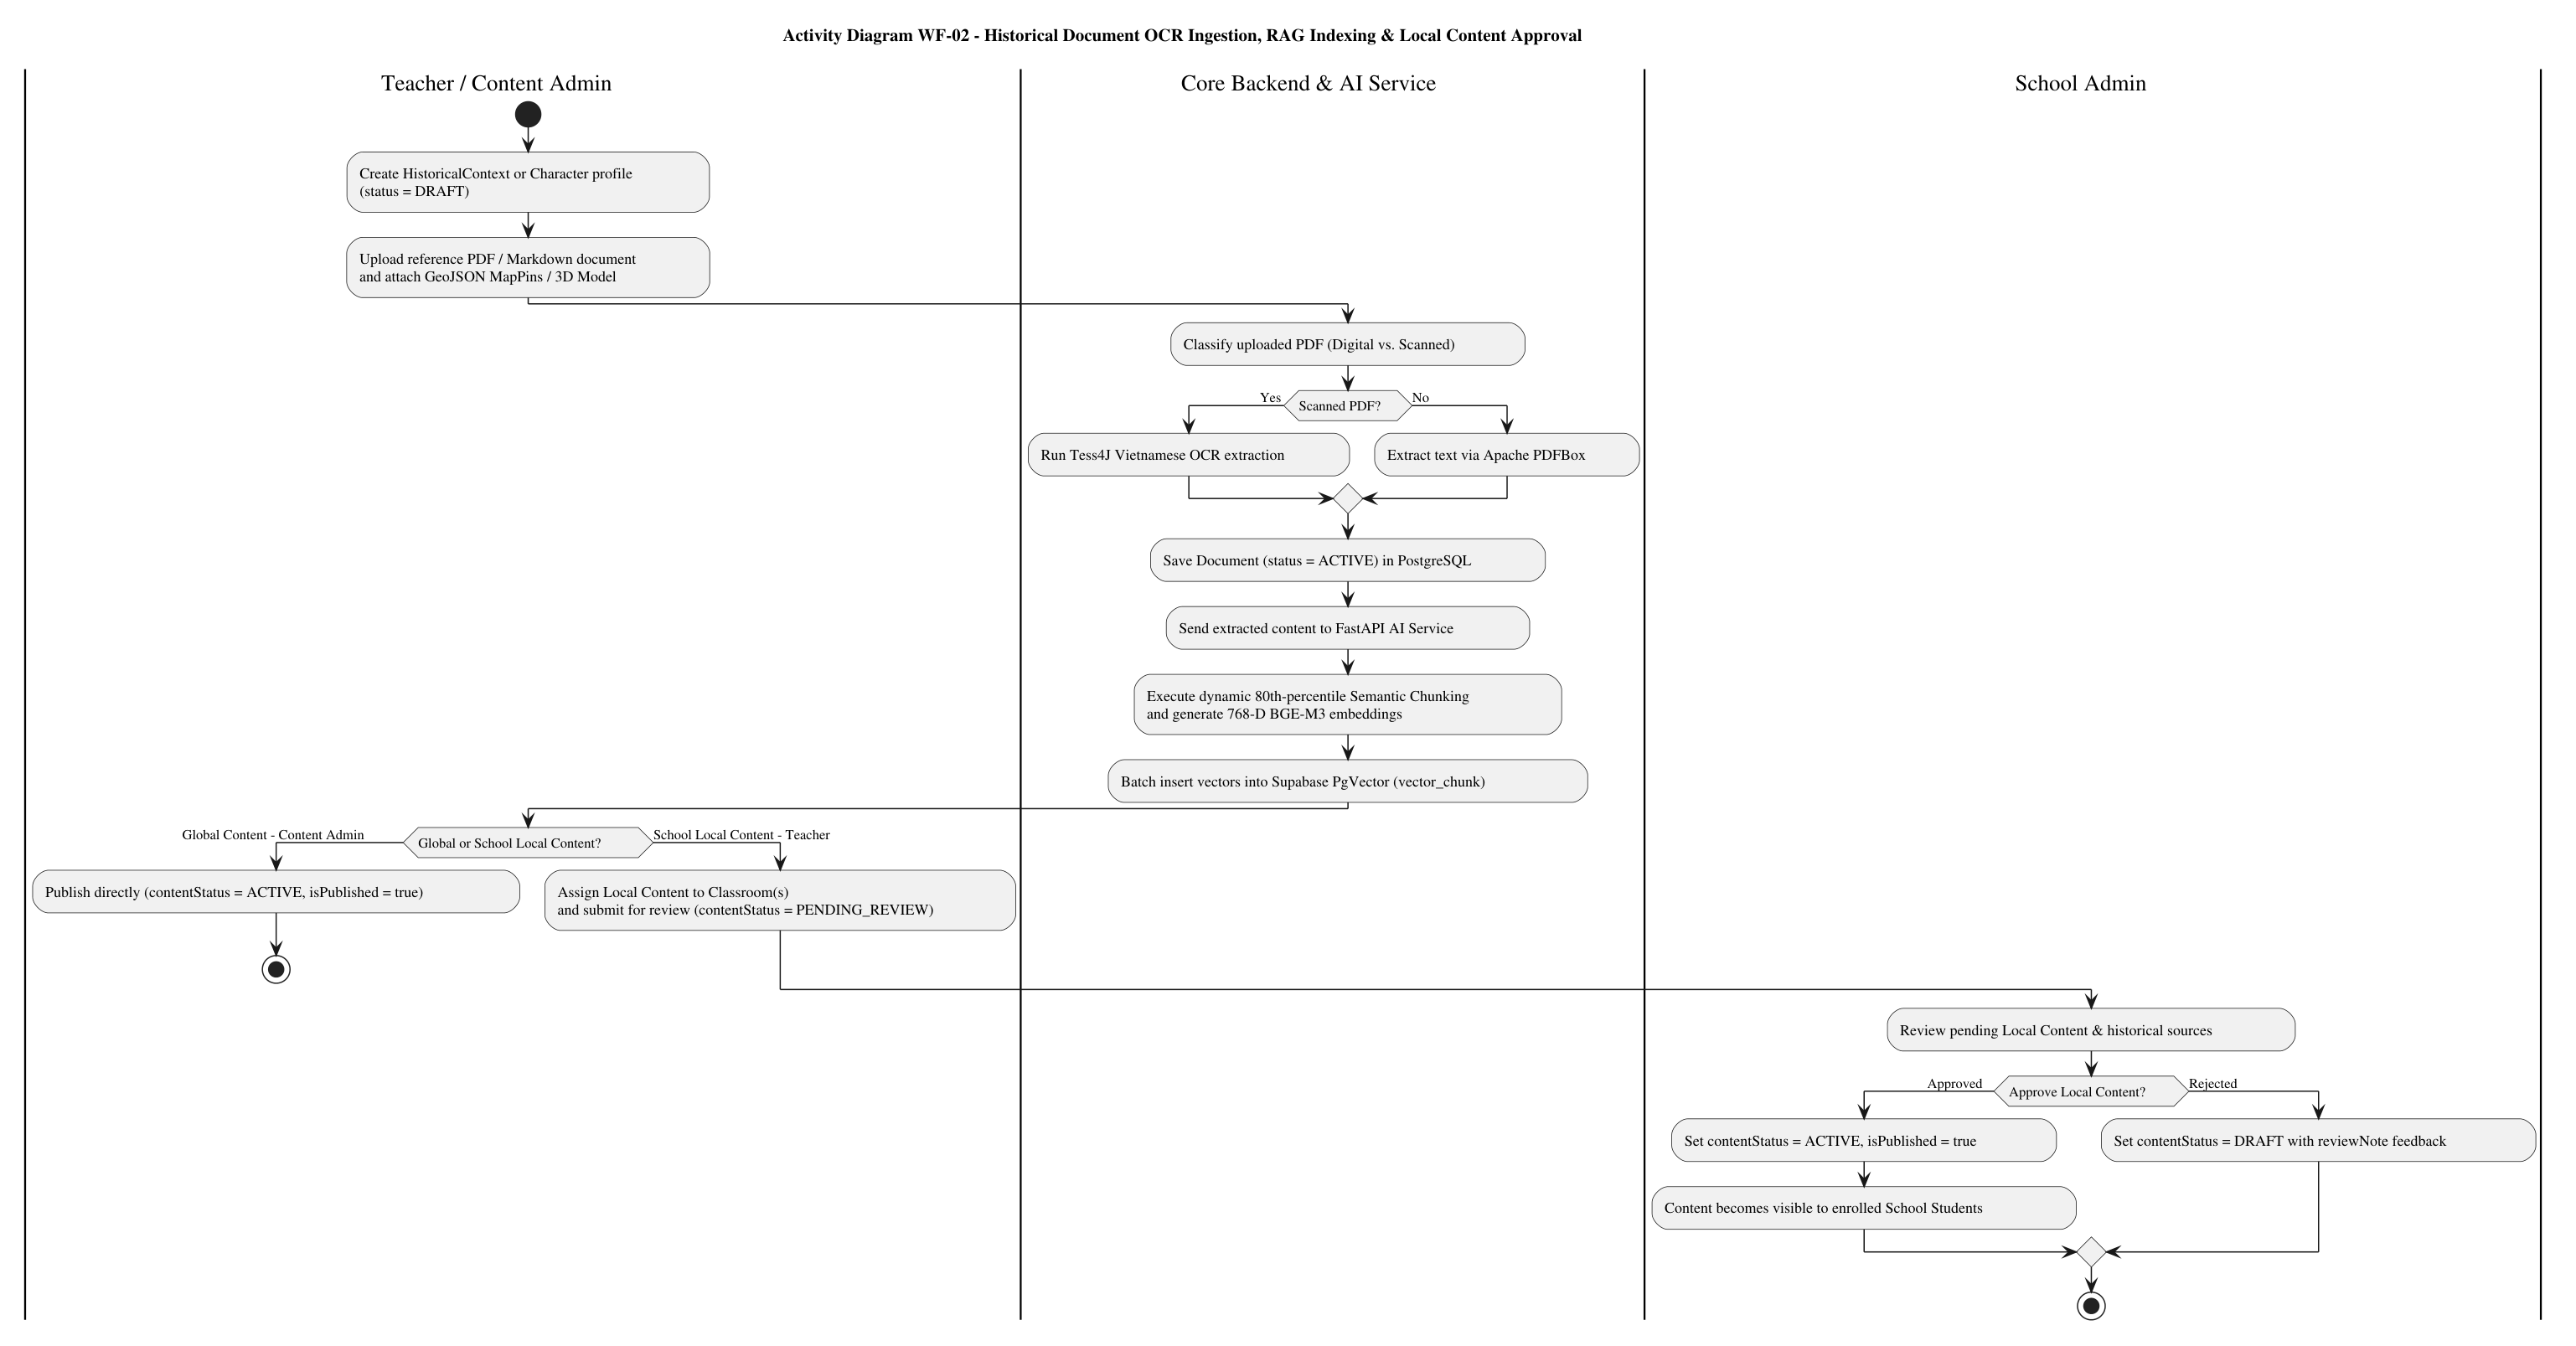
\includegraphics[width=0.95\textwidth,height=0.42\textheight,keepaspectratio]{figures/act_wf02_rag_content_and_local_approval.png}
    \caption{Activity Diagram WF-02 -- Historical Document OCR Ingestion, RAG Indexing and Content Approval}
    \label{fig:act_wf02}
\end{figure}

\begin{figure}[htbp]
    \centering
    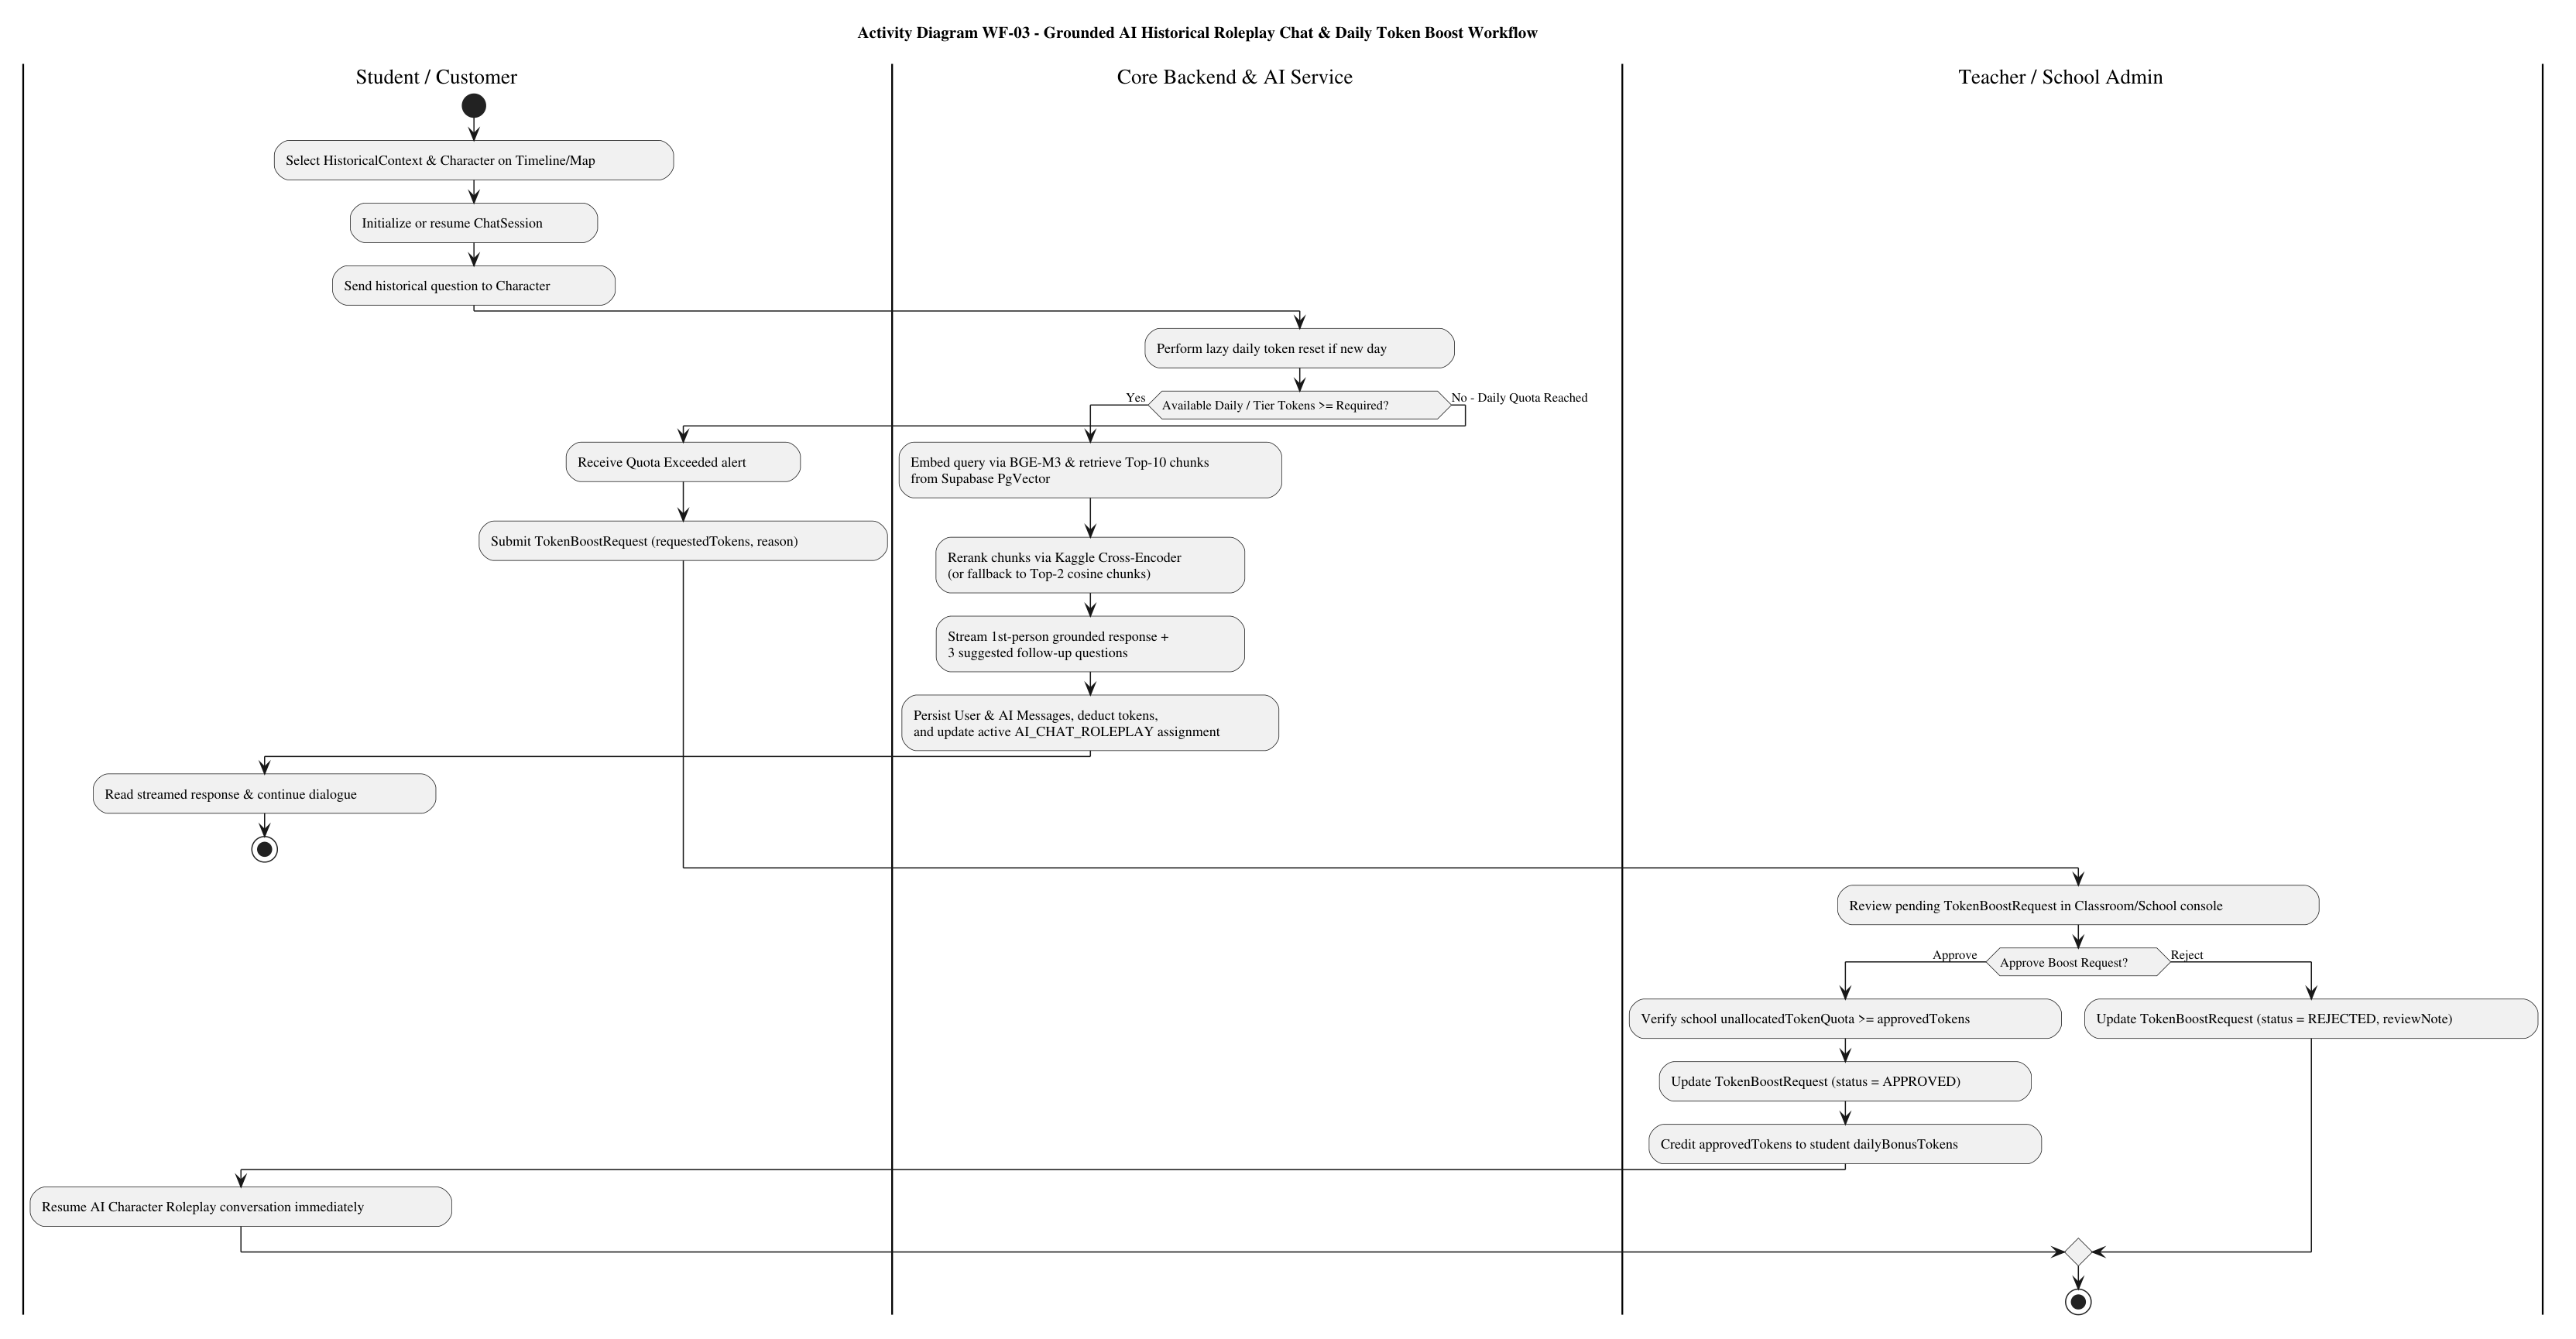
\includegraphics[width=0.95\textwidth,height=0.42\textheight,keepaspectratio]{figures/act_wf03_ai_character_roleplay_and_token_boost.png}
    \caption{Activity Diagram WF-03 -- Grounded AI Historical Roleplay Chat and Daily Token Boost Workflow}
    \label{fig:act_wf03}
\end{figure}

\begin{figure}[htbp]
    \centering
    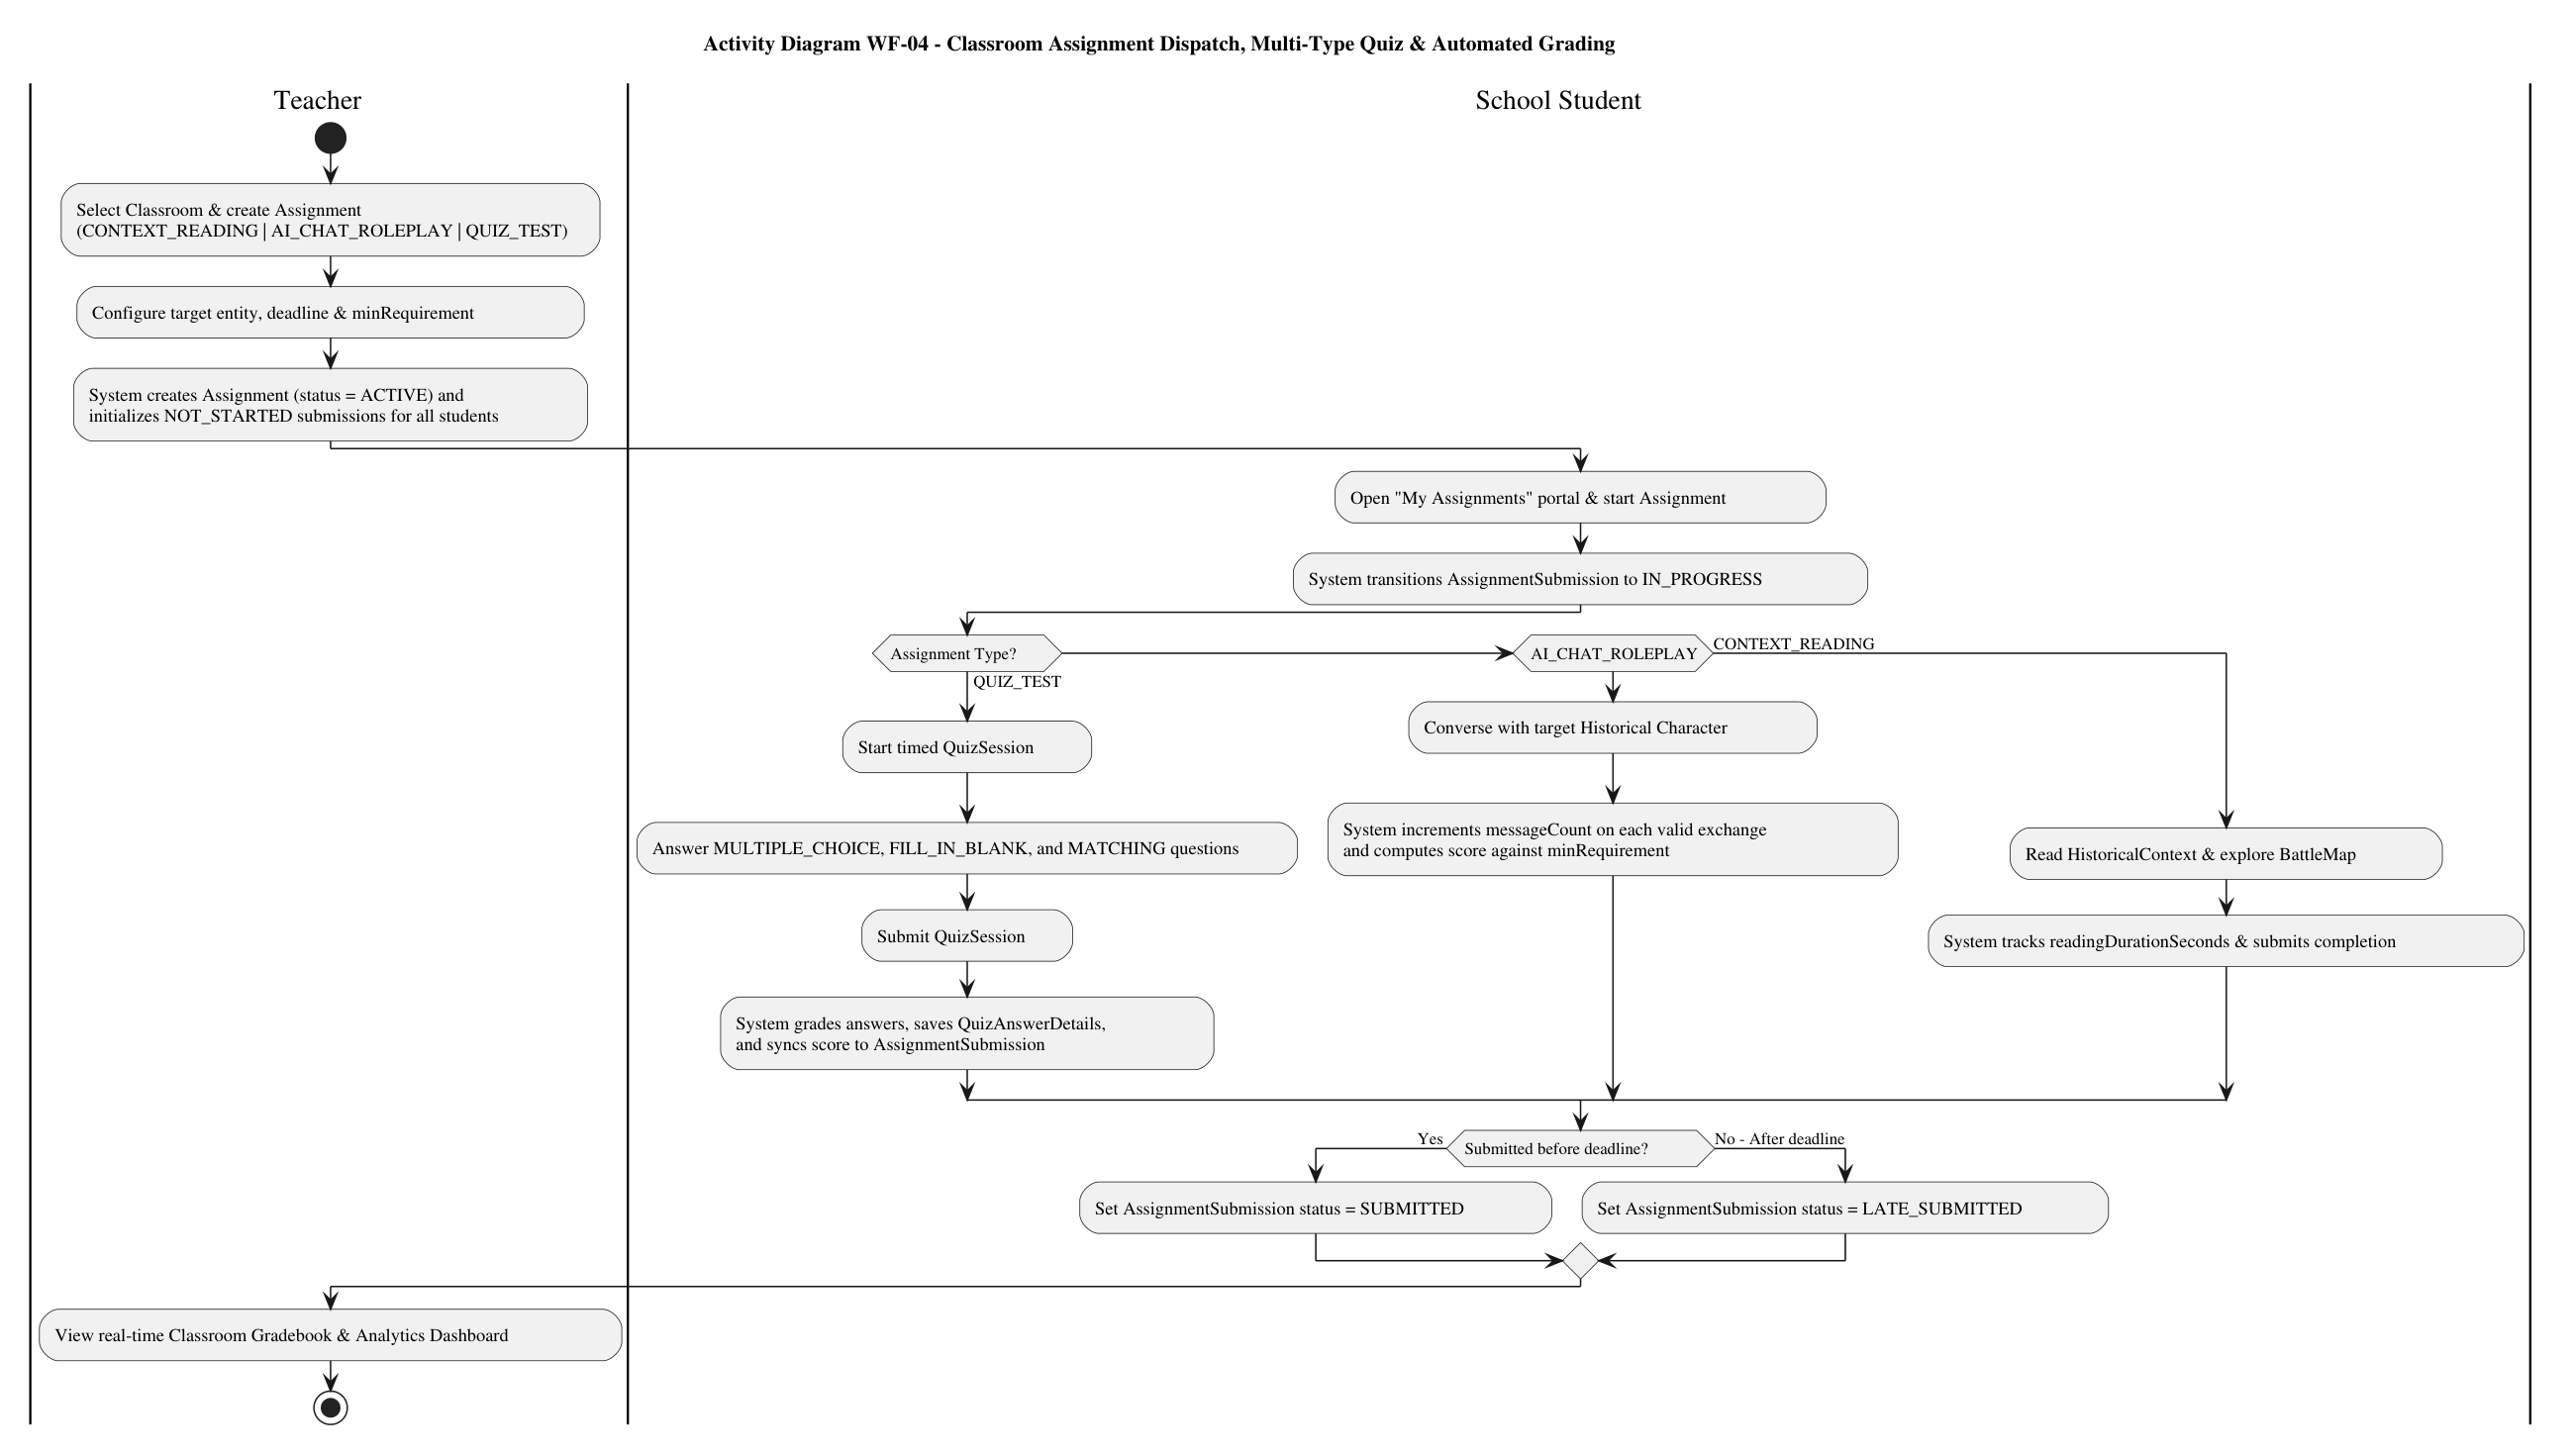
\includegraphics[width=0.95\textwidth,height=0.42\textheight,keepaspectratio]{figures/act_wf04_classroom_assignment_and_quiz_grading.png}
    \caption{Activity Diagram WF-04 -- Classroom Assignment Dispatch, Multi-Type Quiz and Automated Grading}
    \label{fig:act_wf04}
\end{figure}

\begin{figure}[htbp]
    \centering
    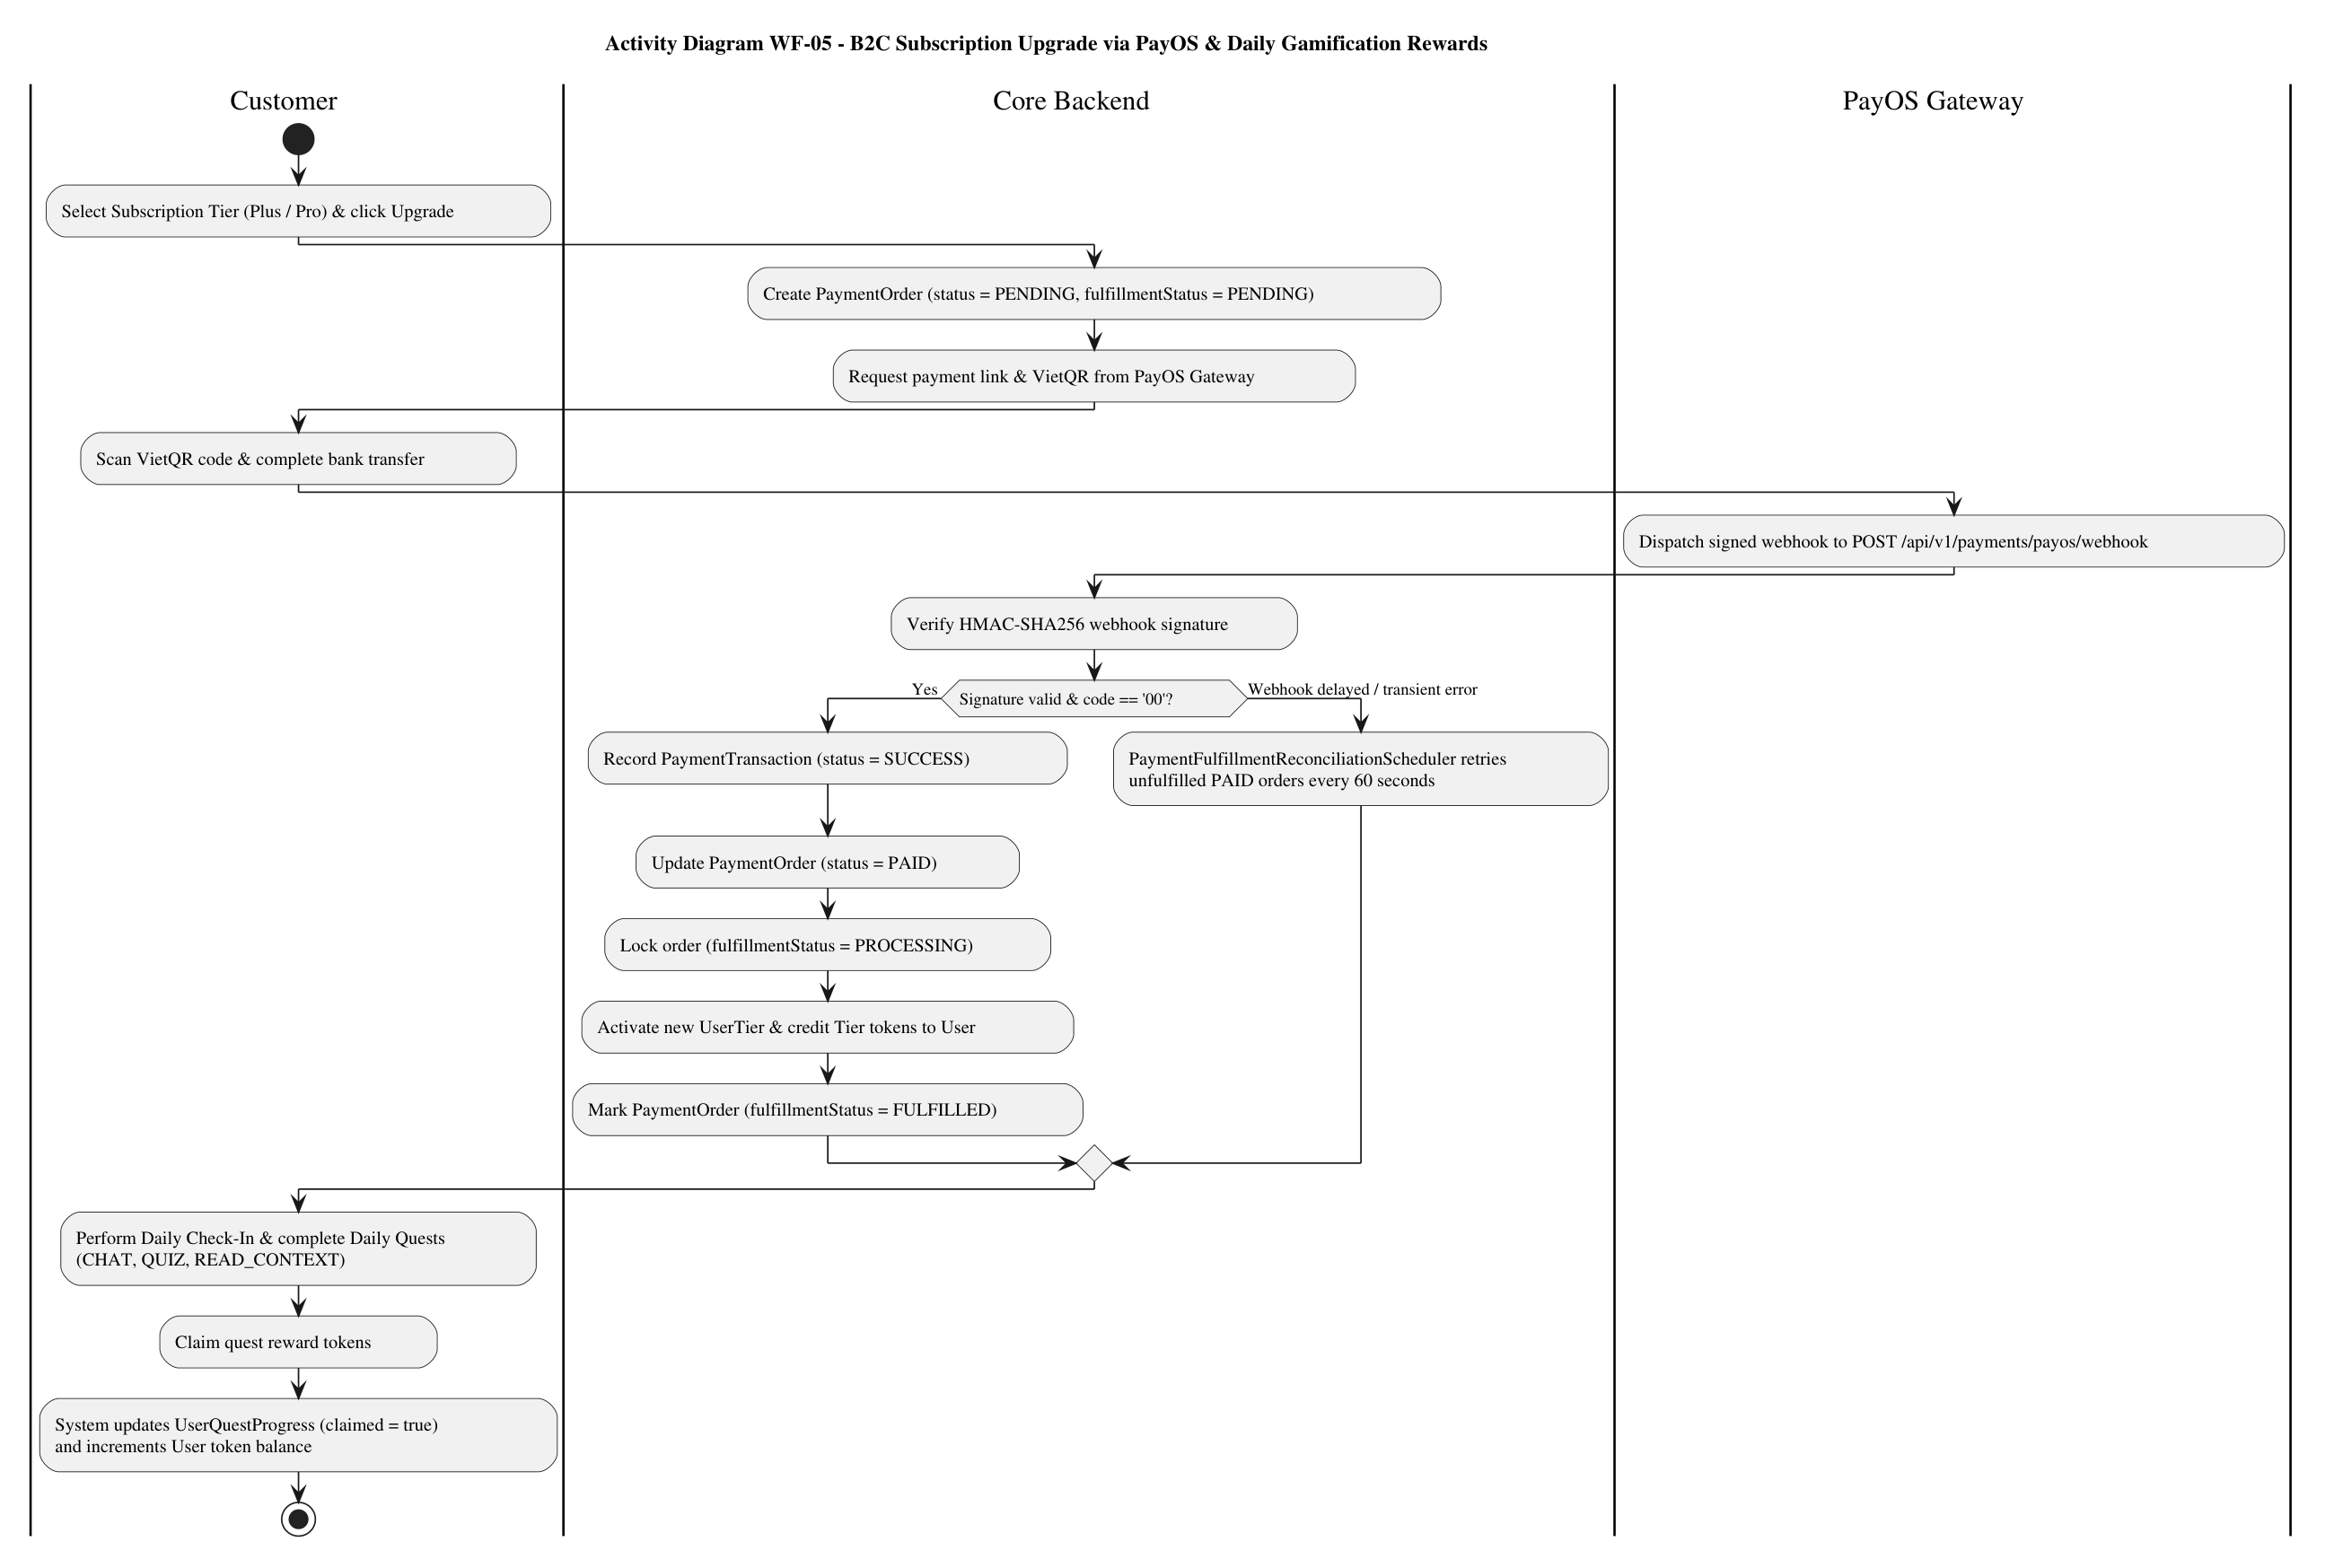
\includegraphics[width=0.95\textwidth,height=0.42\textheight,keepaspectratio]{figures/act_wf05_b2c_payos_subscription_and_gamification.png}
    \caption{Activity Diagram WF-05 -- B2C Subscription Upgrade via PayOS and Daily Gamification Rewards}
    \label{fig:act_wf05}
\end{figure}

\newpage
% ============================================================================
% SECTION 5: TECHNOLOGY & AI / LLM / RAG SPECIFICATION
% ============================================================================
\section{Technology and AI / RAG Specification}

\subsection{System Technology and AI Tool Declaration}

Table~\ref{tab:tech_declaration} declares all third-party services, development technologies, source control and CI/CD pipelines, deployment environments, and AI tools used across the project lifecycle.

\footnotesize
\begin{longtable}{|L{2.9cm}|L{3.8cm}|L{7.6cm}|}
\hline
\rowcolor{tableheader}
\textbf{Category} & \textbf{Component / Service} & \textbf{Purpose, Version \& Data Exchanged} \\
\hline
\endhead

\multirow{7}{2.9cm}{\textbf{1. Third-Party Services}}
& Google OAuth 2.0 (spring-boot-\ab starter-\ab oauth2-client) & Purpose: Single Sign-On (SSO) authentication for Customers.\newline Data Exchanged: OAuth authorization code exchanged for verified user email, display name, and avatar URL. \\
\cline{2-3}
& Cloudflare R2 / Supabase Storage & Purpose: Object storage for uploaded PDF documents, 2D historical illustrations, interactive battle-map rasters, and 3D character models (.glb).\newline Data Exchanged: Binary media streams and presigned upload/view URLs. \\
\cline{2-3}
& PayOS Payment Gateway (payos-java) & Purpose: B2C subscription tier VietQR checkout and webhook payment confirmation.\newline Data Exchanged: Outbound orderCode, amount, and return URLs; Inbound HMAC-SHA256 signed webhook payloads. \\
\cline{2-3}
& SMTP Mail Server (spring-boot-\ab starter-mail) & Purpose: Transactional email delivery for password reset links and initial OAuth/School credentials.\newline Data Exchanged: Recipient email address, reset URL, or temporary password. \\
\cline{2-3}
& Ollama / External OpenAI-Compatible LLM API & Purpose: Conversational AI historical roleplay generation, follow-up question suggestion, and dense text embedding (bge-m3).\newline Data Exchanged: Grounded system prompt, sanitized RAG historical passages, and dialogue turns (no PII or credentials sent). \\
\cline{2-3}
& Kaggle Cross-Encoder Reranker API & Purpose: Reranks candidate vector chunks by semantic relevance to the learner's query.\newline Data Exchanged: User historical question and candidate chunk texts. \\
\cline{2-3}
& Supabase PgVector Cloud (supabase-py) & Purpose: Hosted vector database storing 768-D embeddings and executing cosine similarity searches.\newline Data Exchanged: Document chunk texts, 768-D float vectors, and entity UUID filters. \\
\hline

\multirow{5}{2.9cm}{\textbf{2. Development Technologies}}
& Frontend Web & Next.js / React / TypeScript, TailwindCSS, Axios, Interactive Historical Map UI, 3D Model Viewer (.glb rendering). \\
\cline{2-3}
& Core Backend & Java 21 LTS, Spring Boot 3.2.5, Spring Security 6, Spring Data JPA (Hibernate 6), jjwt 0.12.5, Flyway Core, Lombok, SpringDoc OpenAPI. \\
\cline{2-3}
& Document \& OCR Engine & Apache PDFBox (digital PDF text extraction), Tess4J with vie.traineddata (Vietnamese OCR fallback for scanned PDFs), Apache Commons CSV (bulk roster \& question bank imports). \\
\cline{2-3}
& AI \& RAG Service & Python 3.11+, FastAPI, Uvicorn, httpx, Pydantic / pydantic-\ab settings. \\
\cline{2-3}
& Database \& Observability & PostgreSQL 16, PgVector Extension (HNSW index), Micrometer Prometheus + Prometheus \& Grafana Docker monitoring stack. \\
\hline

\multirow{3}{2.9cm}{\textbf{3. Source Control \& DevOps}}
& Repository \& Branching & Git / GitHub repository. Branching strategy: main (protected release branch), develop, and topic branches (feature/*, fix/*). \\
\cline{2-3}
& CI/CD Pipeline & GitHub Actions automated workflow executing Maven test builds (JUnit 5 + Spring Security Test) for Java Backend and syntax/unit validation for Python AI Service on every pull request and push. \\
\cline{2-3}
& Containerization & Multi-container Docker \& Docker Compose (Dockerfile for Java Backend, Python AI Service, and docker-compose.\ab monitoring.yml for Prometheus/Grafana). \\
\hline

\multirow{3}{2.9cm}{\textbf{4. Deployment Environments}}
& Development (Local) & Local PostgreSQL / Supabase dev schema, Java Spring Boot on port 8080, FastAPI AI service on port 8001, seeded via deterministic SQL scripts. \\
\cline{2-3}
& Staging \& Production & Deployed on AWS EC2 (c6a.large) behind Nginx Reverse Proxy with SSL/TLS termination, Docker Compose management, and PostgreSQL / Supabase PgVector. \\
\cline{2-3}
& Deployment \& Rollback Strategy & Immutable Docker image tags and Flyway versioned schema migrations. Rollback is performed by re-deploying the previous verified Docker image and restoring pre-migration database snapshots if needed. \\
\hline

\multirow{3}{2.9cm}{\textbf{5. AI Tools Used in Development}}
& Specification \& Design & Gemini / Claude / ChatGPT: Assisted in refining SRS use case descriptions, drafting PlantUML (.puml) sequence/class/state diagrams, and formatting LaTeX tables. All outputs were manually verified against business rules. \\
\cline{2-3}
& Coding \& Refactoring & GitHub Copilot / Cursor / Antigravity Coding Agent: Assisted in boilerplate DTO/mapper generation, database migration drafting, and REST API contract alignment. \\
\cline{2-3}
& Testing \& Verification & Assisted in scaffolding JUnit 5 / MockMvc unit and integration test cases for authentication, classroom imports, quiz grading, and payment fulfillment. \\
\hline
\caption{Technology Stack, Infrastructure and AI Tool Usage Declaration}
\label{tab:tech_declaration}
\end{longtable}
\normalsize

\newpage
\subsection{AI and RAG Technical Specification}

Because HistoryTalk incorporates Conversational AI and Retrieval-Augmented Generation (RAG) as a core product capability, this section documents the AI and RAG engineering specifications of the platform.

\begin{figure}[htbp]
    \centering
    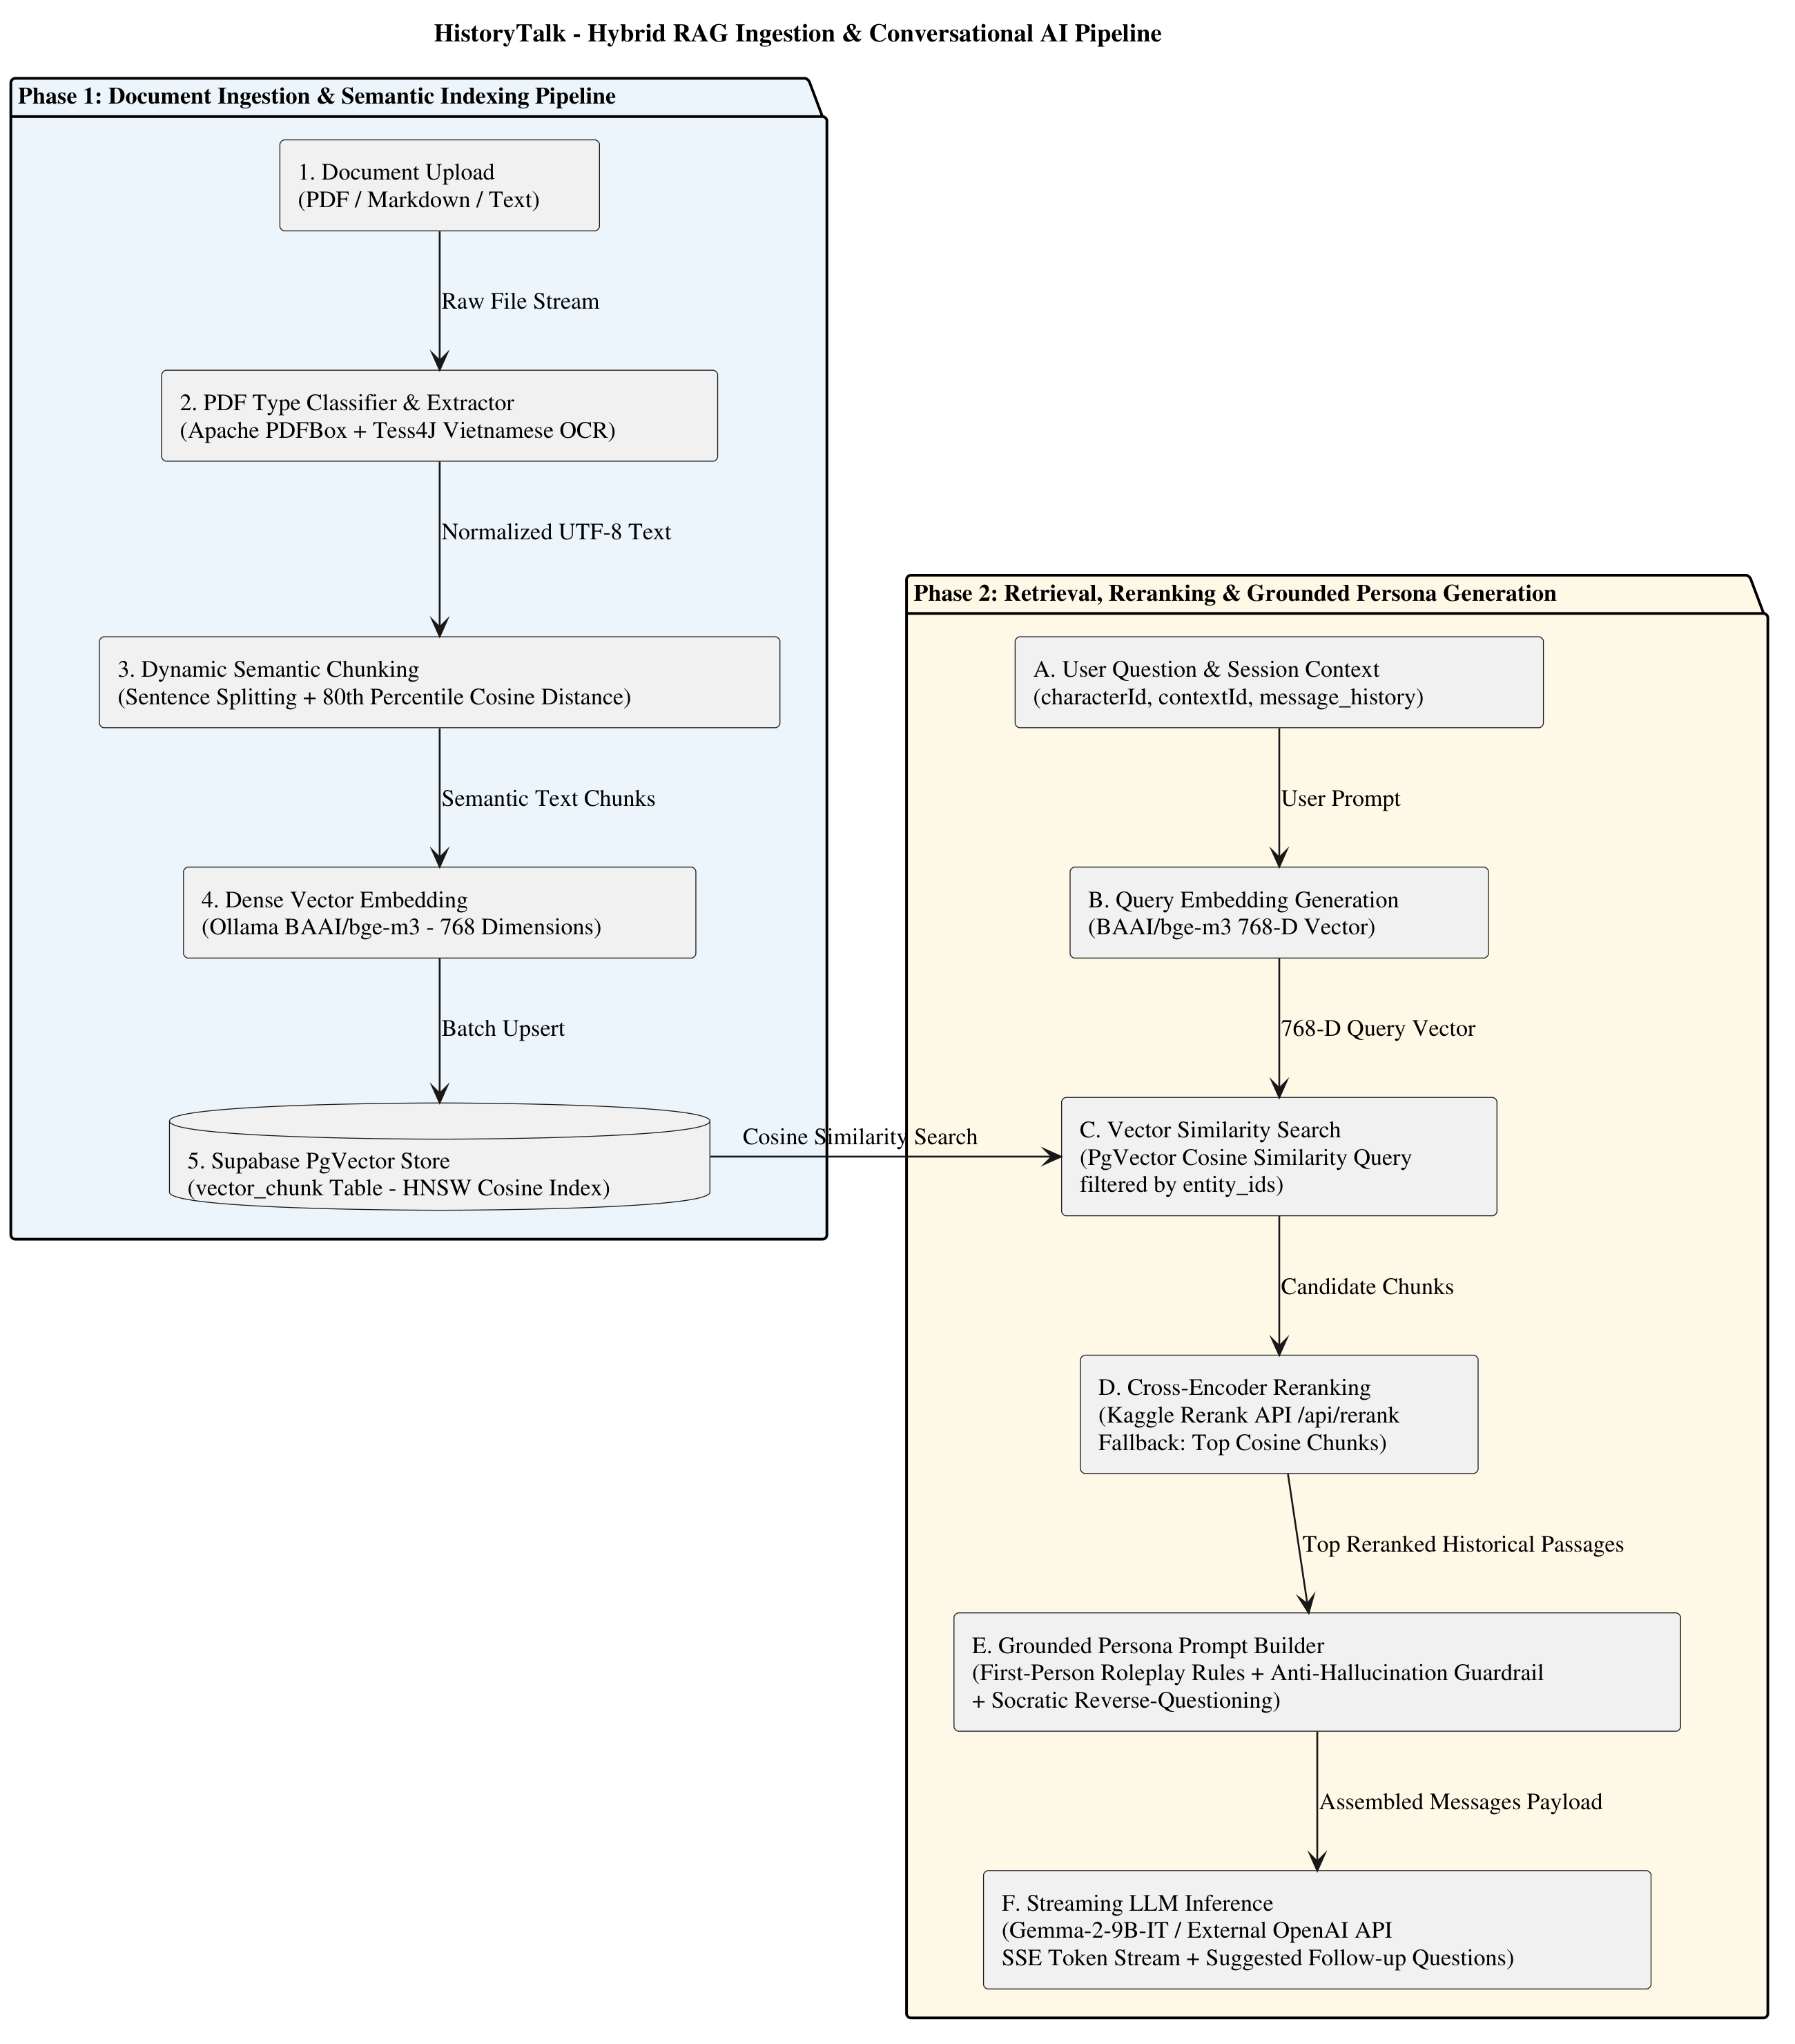
\includegraphics[width=0.92\textwidth,height=0.68\textheight,keepaspectratio]{figures/arch_ai_rag_pipeline.png}
    \caption{Hybrid RAG Document Ingestion and Conversational AI Roleplay Pipeline Architecture}
    \label{fig:arch_ai_rag_pipeline}
\end{figure}

\begin{longtable}{|C{0.7cm}|L{3.3cm}|L{10.3cm}|}
\hline
\rowcolor{tableheader}
\textbf{\#} & \textbf{Specification Item} & \textbf{HistoryTalk Implementation Details} \\
\hline
\endhead

1 & AI / RAG Architecture Diagram & Modeled in Figure~\ref{fig:arch_ai_rag_pipeline} and Sequence Diagram Figure~\ref{fig:seq_07_ai_roleplay_chat_rag}, separating Phase 1 (Asynchronous PDF/OCR Ingestion \& Semantic Vector Indexing) from Phase 2 (Low-Latency Hybrid Vector Retrieval, Cross-Encoder Reranking \& SSE Streaming Persona Inference). \\
\hline

2 & Models \& Versions &
$\bullet$ Primary Roleplay \& Title LLM: Gemma-2-9B-IT (hosted via Ollama with num\_ctx=8192, temperature=0.3, repeat\_penalty=1.15) and configurable External OpenAI-Compatible API (LLM\_PROVIDER=\ab ollama|external in settings.py).\newline
$\bullet$ Dense Embedding Model: BAAI/bge-m3 (768-dimensional multilingual dense embeddings optimized for Vietnamese historical terminology).\newline
$\bullet$ Cross-Encoder Reranker: Hosted Kaggle Cross-Encoder Reranker (/api/rerank) scoring query--passage pairs.\newline
$\bullet$ Document OCR Model: Tesseract 5 / Tess4J with Vietnamese language pack (vie.traineddata). \\
\hline

3 & End-to-End RAG Pipeline &
$\bullet$ Step 1 -- Hybrid Extraction: PdfType\ab Classifier inspects uploaded PDFs; digital PDFs are extracted via Apache PDFBox, whereas scanned archival PDFs are routed to OcrServiceImpl (Tess4J).\newline
$\bullet$ Step 2 -- Dynamic Semantic Chunking (\_semantic\_\ab chunking): Splits text into sentences, computes bge-m3 embeddings, calculates cosine distances between adjacent sentences, and splits chunks dynamically at the 80th percentile distance threshold ($\ge 0.35$) or max\_chunk\_\ab chars = 1200.\newline
$\bullet$ Step 3 -- Vector Indexing: Generates 768-D embeddings and batch-inserts into vector\_chunk indexed with PgVector HNSW (m = 16, ef\_\ab construction = 64).\newline
$\bullet$ Step 4 -- Filtered Retrieval \& Reranking (retrieve\_\ab history\_\ab context): Embeds the user query, performs vector similarity search in Supabase PgVector (filtered by characterId, contextId, and linked context/event UUIDs), and reranks the top candidate chunks via the Kaggle Reranker API.\newline
$\bullet$ Step 5 -- Grounded Persona Prompting \& Socratic Dialogue: Injects retrieved passages into build\_chat\_\ab system\_prompt, enforces first-person Vietnamese pronouns (\vn{\textit{Ta, Trẫm, Tôi}}), applies a 30\% probability Socratic reverse-questioning directive on follow-up turns, streams tokens via SSE, and generates 3 suggested follow-up questions. \\
\hline

4 & Evaluation Metrics \& Target Thresholds &
$\bullet$ Streaming Latency (TTFT): Time-To-First-Token $< 1.5\text{s}$ (95th percentile) under concurrent classroom load, monitored via AiMetrics\ab Service and Prometheus.\newline
$\bullet$ Historical Faithfulness / Groundedness: $\ge 95\%$ of factual claims in character responses must trace directly to retrieved quotes\_used from vector\_chunk or verified character biography.\newline
$\bullet$ Out-of-Domain / Anti-Hallucination Refusal Rate: $100\%$ refusal accuracy on anachronistic or unverified prompts (must acknowledge \vn{\textit{``Sử sách không ghi chép''}} instead of fabricating dates or events).\newline
$\bullet$ Retrieval Recall@10: $\ge 90\%$ recall of ground-truth historical passages on benchmark Vietnamese history QA pairs. \\
\hline

5 & Fallback \& Resilience Mechanisms &
$\bullet$ Reranker Failure Fallback: If the Kaggle Reranker API times out or returns HTTP 5xx, retrieve\_\ab history\_\ab context automatically falls back to the top chunks by PgVector cosine similarity without failing the chat request.\newline
$\bullet$ Embedding Endpoint Fallback \& Backoff: get\_embedding\_\ab from\_ollama implements 3-attempt exponential backoff ($1\text{s}, 2\text{s}, 3\text{s}$) and automatically falls back from /api/embeddings to /api/embed on HTTP 404.\newline
$\bullet$ Dual LLM Provider Routing: Supports zero-code switching between self-hosted Ollama and external OpenAI-compatible endpoints via environment configuration (LLM\_PROVIDER).\newline
$\bullet$ Zero-Hallucination Prompt Guardrail: When rag\_context is empty or does not contain the requested fact, strict RAG Instruction \#3 forces the character to state that historical records do not mention the detail rather than guessing. \\
\hline
\caption{Technical Specification for Conversational AI and Hybrid RAG}
\label{tab:ai_rag_spec}
\end{longtable}


\end{document}
